\PassOptionsToPackage{unicode=true}{hyperref} % options for packages loaded elsewhere
\PassOptionsToPackage{hyphens}{url}
%
\documentclass[]{article}
\usepackage{lmodern}
\usepackage{amssymb,amsmath}
\usepackage{ifxetex,ifluatex}
\usepackage{fixltx2e} % provides \textsubscript
\ifnum 0\ifxetex 1\fi\ifluatex 1\fi=0 % if pdftex
  \usepackage[T1]{fontenc}
  \usepackage[utf8]{inputenc}
  \usepackage{textcomp} % provides euro and other symbols
\else % if luatex or xelatex
  \usepackage{unicode-math}
  \defaultfontfeatures{Ligatures=TeX,Scale=MatchLowercase}
\fi
% use upquote if available, for straight quotes in verbatim environments
\IfFileExists{upquote.sty}{\usepackage{upquote}}{}
% use microtype if available
\IfFileExists{microtype.sty}{%
\usepackage[]{microtype}
\UseMicrotypeSet[protrusion]{basicmath} % disable protrusion for tt fonts
}{}
\IfFileExists{parskip.sty}{%
\usepackage{parskip}
}{% else
\setlength{\parindent}{0pt}
\setlength{\parskip}{6pt plus 2pt minus 1pt}
}
\usepackage{hyperref}
\hypersetup{
            pdftitle={Final Project EDA},
            pdfborder={0 0 0},
            breaklinks=true}
\urlstyle{same}  % don't use monospace font for urls
\usepackage[margin=1in]{geometry}
\usepackage{color}
\usepackage{fancyvrb}
\newcommand{\VerbBar}{|}
\newcommand{\VERB}{\Verb[commandchars=\\\{\}]}
\DefineVerbatimEnvironment{Highlighting}{Verbatim}{commandchars=\\\{\}}
% Add ',fontsize=\small' for more characters per line
\usepackage{framed}
\definecolor{shadecolor}{RGB}{248,248,248}
\newenvironment{Shaded}{\begin{snugshade}}{\end{snugshade}}
\newcommand{\AlertTok}[1]{\textcolor[rgb]{0.94,0.16,0.16}{#1}}
\newcommand{\AnnotationTok}[1]{\textcolor[rgb]{0.56,0.35,0.01}{\textbf{\textit{#1}}}}
\newcommand{\AttributeTok}[1]{\textcolor[rgb]{0.77,0.63,0.00}{#1}}
\newcommand{\BaseNTok}[1]{\textcolor[rgb]{0.00,0.00,0.81}{#1}}
\newcommand{\BuiltInTok}[1]{#1}
\newcommand{\CharTok}[1]{\textcolor[rgb]{0.31,0.60,0.02}{#1}}
\newcommand{\CommentTok}[1]{\textcolor[rgb]{0.56,0.35,0.01}{\textit{#1}}}
\newcommand{\CommentVarTok}[1]{\textcolor[rgb]{0.56,0.35,0.01}{\textbf{\textit{#1}}}}
\newcommand{\ConstantTok}[1]{\textcolor[rgb]{0.00,0.00,0.00}{#1}}
\newcommand{\ControlFlowTok}[1]{\textcolor[rgb]{0.13,0.29,0.53}{\textbf{#1}}}
\newcommand{\DataTypeTok}[1]{\textcolor[rgb]{0.13,0.29,0.53}{#1}}
\newcommand{\DecValTok}[1]{\textcolor[rgb]{0.00,0.00,0.81}{#1}}
\newcommand{\DocumentationTok}[1]{\textcolor[rgb]{0.56,0.35,0.01}{\textbf{\textit{#1}}}}
\newcommand{\ErrorTok}[1]{\textcolor[rgb]{0.64,0.00,0.00}{\textbf{#1}}}
\newcommand{\ExtensionTok}[1]{#1}
\newcommand{\FloatTok}[1]{\textcolor[rgb]{0.00,0.00,0.81}{#1}}
\newcommand{\FunctionTok}[1]{\textcolor[rgb]{0.00,0.00,0.00}{#1}}
\newcommand{\ImportTok}[1]{#1}
\newcommand{\InformationTok}[1]{\textcolor[rgb]{0.56,0.35,0.01}{\textbf{\textit{#1}}}}
\newcommand{\KeywordTok}[1]{\textcolor[rgb]{0.13,0.29,0.53}{\textbf{#1}}}
\newcommand{\NormalTok}[1]{#1}
\newcommand{\OperatorTok}[1]{\textcolor[rgb]{0.81,0.36,0.00}{\textbf{#1}}}
\newcommand{\OtherTok}[1]{\textcolor[rgb]{0.56,0.35,0.01}{#1}}
\newcommand{\PreprocessorTok}[1]{\textcolor[rgb]{0.56,0.35,0.01}{\textit{#1}}}
\newcommand{\RegionMarkerTok}[1]{#1}
\newcommand{\SpecialCharTok}[1]{\textcolor[rgb]{0.00,0.00,0.00}{#1}}
\newcommand{\SpecialStringTok}[1]{\textcolor[rgb]{0.31,0.60,0.02}{#1}}
\newcommand{\StringTok}[1]{\textcolor[rgb]{0.31,0.60,0.02}{#1}}
\newcommand{\VariableTok}[1]{\textcolor[rgb]{0.00,0.00,0.00}{#1}}
\newcommand{\VerbatimStringTok}[1]{\textcolor[rgb]{0.31,0.60,0.02}{#1}}
\newcommand{\WarningTok}[1]{\textcolor[rgb]{0.56,0.35,0.01}{\textbf{\textit{#1}}}}
\usepackage{graphicx,grffile}
\makeatletter
\def\maxwidth{\ifdim\Gin@nat@width>\linewidth\linewidth\else\Gin@nat@width\fi}
\def\maxheight{\ifdim\Gin@nat@height>\textheight\textheight\else\Gin@nat@height\fi}
\makeatother
% Scale images if necessary, so that they will not overflow the page
% margins by default, and it is still possible to overwrite the defaults
% using explicit options in \includegraphics[width, height, ...]{}
\setkeys{Gin}{width=\maxwidth,height=\maxheight,keepaspectratio}
\setlength{\emergencystretch}{3em}  % prevent overfull lines
\providecommand{\tightlist}{%
  \setlength{\itemsep}{0pt}\setlength{\parskip}{0pt}}
\setcounter{secnumdepth}{0}
% Redefines (sub)paragraphs to behave more like sections
\ifx\paragraph\undefined\else
\let\oldparagraph\paragraph
\renewcommand{\paragraph}[1]{\oldparagraph{#1}\mbox{}}
\fi
\ifx\subparagraph\undefined\else
\let\oldsubparagraph\subparagraph
\renewcommand{\subparagraph}[1]{\oldsubparagraph{#1}\mbox{}}
\fi

% set default figure placement to htbp
\makeatletter
\def\fps@figure{htbp}
\makeatother

\usepackage{booktabs}
\usepackage{longtable}
\usepackage{array}
\usepackage{multirow}
\usepackage{wrapfig}
\usepackage{float}
\usepackage{colortbl}
\usepackage{pdflscape}
\usepackage{tabu}
\usepackage{threeparttable}
\usepackage{threeparttablex}
\usepackage[normalem]{ulem}
\usepackage{makecell}
\usepackage{xcolor}

\title{Final Project EDA}
\author{}
\date{\vspace{-2.5em}}

\begin{document}
\maketitle

\begin{Shaded}
\begin{Highlighting}[]
\CommentTok{# load all necessary libraries}
\KeywordTok{library}\NormalTok{(mltools)}
\KeywordTok{library}\NormalTok{(data.table)}
\KeywordTok{library}\NormalTok{(dplyr)}
\end{Highlighting}
\end{Shaded}

\begin{verbatim}
## 
## Attaching package: 'dplyr'
\end{verbatim}

\begin{verbatim}
## The following objects are masked from 'package:data.table':
## 
##     between, first, last
\end{verbatim}

\begin{verbatim}
## The following objects are masked from 'package:stats':
## 
##     filter, lag
\end{verbatim}

\begin{verbatim}
## The following objects are masked from 'package:base':
## 
##     intersect, setdiff, setequal, union
\end{verbatim}

\begin{Shaded}
\begin{Highlighting}[]
\KeywordTok{library}\NormalTok{(stringr)}
\KeywordTok{library}\NormalTok{(klaR)}
\end{Highlighting}
\end{Shaded}

\begin{verbatim}
## Loading required package: MASS
\end{verbatim}

\begin{verbatim}
## 
## Attaching package: 'MASS'
\end{verbatim}

\begin{verbatim}
## The following object is masked from 'package:dplyr':
## 
##     select
\end{verbatim}

\begin{Shaded}
\begin{Highlighting}[]
\KeywordTok{library}\NormalTok{(gapminder)}
\KeywordTok{library}\NormalTok{(ggplot2)}
\KeywordTok{library}\NormalTok{(dendextend)}
\end{Highlighting}
\end{Shaded}

\begin{verbatim}
## 
## ---------------------
## Welcome to dendextend version 1.15.2
## Type citation('dendextend') for how to cite the package.
## 
## Type browseVignettes(package = 'dendextend') for the package vignette.
## The github page is: https://github.com/talgalili/dendextend/
## 
## Suggestions and bug-reports can be submitted at: https://github.com/talgalili/dendextend/issues
## You may ask questions at stackoverflow, use the r and dendextend tags: 
##   https://stackoverflow.com/questions/tagged/dendextend
## 
##  To suppress this message use:  suppressPackageStartupMessages(library(dendextend))
## ---------------------
\end{verbatim}

\begin{verbatim}
## 
## Attaching package: 'dendextend'
\end{verbatim}

\begin{verbatim}
## The following object is masked from 'package:data.table':
## 
##     set
\end{verbatim}

\begin{verbatim}
## The following object is masked from 'package:stats':
## 
##     cutree
\end{verbatim}

\begin{Shaded}
\begin{Highlighting}[]
\KeywordTok{library}\NormalTok{(Hmisc)}
\end{Highlighting}
\end{Shaded}

\begin{verbatim}
## Loading required package: lattice
\end{verbatim}

\begin{verbatim}
## Loading required package: survival
\end{verbatim}

\begin{verbatim}
## Loading required package: Formula
\end{verbatim}

\begin{verbatim}
## 
## Attaching package: 'Hmisc'
\end{verbatim}

\begin{verbatim}
## The following objects are masked from 'package:dplyr':
## 
##     src, summarize
\end{verbatim}

\begin{verbatim}
## The following objects are masked from 'package:base':
## 
##     format.pval, units
\end{verbatim}

\begin{Shaded}
\begin{Highlighting}[]
\KeywordTok{library}\NormalTok{(mlbench)}
\KeywordTok{library}\NormalTok{(caret)}
\end{Highlighting}
\end{Shaded}

\begin{verbatim}
## 
## Attaching package: 'caret'
\end{verbatim}

\begin{verbatim}
## The following object is masked from 'package:survival':
## 
##     cluster
\end{verbatim}

\begin{Shaded}
\begin{Highlighting}[]
\KeywordTok{library}\NormalTok{(factoextra)}
\end{Highlighting}
\end{Shaded}

\begin{verbatim}
## Welcome! Want to learn more? See two factoextra-related books at https://goo.gl/ve3WBa
\end{verbatim}

\begin{Shaded}
\begin{Highlighting}[]
\KeywordTok{library}\NormalTok{(NbClust)}
\KeywordTok{library}\NormalTok{(fossil)}
\end{Highlighting}
\end{Shaded}

\begin{verbatim}
## Loading required package: sp
\end{verbatim}

\begin{verbatim}
## Loading required package: maps
\end{verbatim}

\begin{verbatim}
## Loading required package: shapefiles
\end{verbatim}

\begin{verbatim}
## Loading required package: foreign
\end{verbatim}

\begin{verbatim}
## 
## Attaching package: 'shapefiles'
\end{verbatim}

\begin{verbatim}
## The following objects are masked from 'package:foreign':
## 
##     read.dbf, write.dbf
\end{verbatim}

\begin{Shaded}
\begin{Highlighting}[]
\KeywordTok{library}\NormalTok{(countrycode)}
\KeywordTok{library}\NormalTok{(tidyverse)}
\end{Highlighting}
\end{Shaded}

\begin{verbatim}
## -- Attaching packages --------------------------------------- tidyverse 1.3.1 --
\end{verbatim}

\begin{verbatim}
## v tibble  3.1.6     v purrr   0.3.4
## v tidyr   1.2.0     v forcats 0.5.1
## v readr   2.1.2
\end{verbatim}

\begin{verbatim}
## -- Conflicts ------------------------------------------ tidyverse_conflicts() --
## x dplyr::between()    masks data.table::between()
## x dplyr::filter()     masks stats::filter()
## x dplyr::first()      masks data.table::first()
## x dplyr::lag()        masks stats::lag()
## x dplyr::last()       masks data.table::last()
## x purrr::lift()       masks caret::lift()
## x purrr::map()        masks maps::map()
## x tidyr::replace_na() masks mltools::replace_na()
## x MASS::select()      masks dplyr::select()
## x Hmisc::src()        masks dplyr::src()
## x Hmisc::summarize()  masks dplyr::summarize()
## x purrr::transpose()  masks data.table::transpose()
\end{verbatim}

\begin{Shaded}
\begin{Highlighting}[]
\KeywordTok{library}\NormalTok{(ggrepel)}
\KeywordTok{library}\NormalTok{(kableExtra)}
\end{Highlighting}
\end{Shaded}

\begin{verbatim}
## 
## Attaching package: 'kableExtra'
\end{verbatim}

\begin{verbatim}
## The following object is masked from 'package:dplyr':
## 
##     group_rows
\end{verbatim}

\begin{Shaded}
\begin{Highlighting}[]
\KeywordTok{library}\NormalTok{(cluster)}
\end{Highlighting}
\end{Shaded}

\begin{verbatim}
## 
## Attaching package: 'cluster'
\end{verbatim}

\begin{verbatim}
## The following object is masked from 'package:maps':
## 
##     votes.repub
\end{verbatim}

\begin{Shaded}
\begin{Highlighting}[]
\KeywordTok{library}\NormalTok{(xtable)}
\end{Highlighting}
\end{Shaded}

\begin{verbatim}
## 
## Attaching package: 'xtable'
\end{verbatim}

\begin{verbatim}
## The following objects are masked from 'package:Hmisc':
## 
##     label, label<-
\end{verbatim}

\begin{Shaded}
\begin{Highlighting}[]
\CommentTok{# read in data, and summarize}
\NormalTok{data <-}\StringTok{ }\KeywordTok{read.csv}\NormalTok{(}\StringTok{'data/immigration_policies/policy_list.csv'}\NormalTok{)}
\KeywordTok{summary}\NormalTok{(data)}
\end{Highlighting}
\end{Shaded}

\begin{verbatim}
##       ID            COUNTRY_NAME           ISO3               ISO2          
##  Length:1762        Length:1762        Length:1762        Length:1762       
##  Class :character   Class :character   Class :character   Class :character  
##  Mode  :character   Mode  :character   Mode  :character   Mode  :character  
##                                                                             
##                                                                             
##                                                                             
##  POLICY_TYPE        POLICY_SUBTYPE      START_DATE          END_DATE        
##  Length:1762        Length:1762        Length:1762        Length:1762       
##  Class :character   Class :character   Class :character   Class :character  
##  Mode  :character   Mode  :character   Mode  :character   Mode  :character  
##                                                                             
##                                                                             
##                                                                             
##       AIR          AIR_TYPE         TARGETS_AIR             LAND       
##  Min.   :0.000   Length:1762        Length:1762        Min.   :0.0000  
##  1st Qu.:0.000   Class :character   Class :character   1st Qu.:0.0000  
##  Median :0.000   Mode  :character   Mode  :character   Median :0.0000  
##  Mean   :0.391                                         Mean   :0.1425  
##  3rd Qu.:1.000                                         3rd Qu.:0.0000  
##  Max.   :1.000                                         Max.   :1.0000  
##   LAND_TYPE         TARGETS_LAND            SEA           SEA_TYPE        
##  Length:1762        Length:1762        Min.   :0.0000   Length:1762       
##  Class :character   Class :character   1st Qu.:0.0000   Class :character  
##  Mode  :character   Mode  :character   Median :0.0000   Mode  :character  
##                                        Mean   :0.1294                     
##                                        3rd Qu.:0.0000                     
##                                        Max.   :1.0000                     
##  TARGETS_SEA           CITIZEN       CITIZEN_LIST        HISTORY_BAN    
##  Length:1762        Min.   :0.0000   Length:1762        Min.   :0.0000  
##  Class :character   1st Qu.:0.0000   Class :character   1st Qu.:0.0000  
##  Mode  :character   Median :0.0000   Mode  :character   Median :0.0000  
##                     Mean   :0.1101                      Mean   :0.1532  
##                     3rd Qu.:0.0000                      3rd Qu.:0.0000  
##                     Max.   :1.0000                      Max.   :1.0000  
##  HISTORY_BAN_LIST      REFUGEE         REFUGEE_LIST          VISA_BAN      
##  Length:1762        Min.   :0.000000   Length:1762        Min.   :0.00000  
##  Class :character   1st Qu.:0.000000   Class :character   1st Qu.:0.00000  
##  Mode  :character   Median :0.000000   Mode  :character   Median :0.00000  
##                     Mean   :0.001703                      Mean   :0.03575  
##                     3rd Qu.:0.000000                      3rd Qu.:0.00000  
##                     Max.   :1.000000                      Max.   :1.00000  
##  VISA_BAN_TYPE      VISA_BAN_LIST      CITIZEN_EXCEP    CITIZEN_EXCEP_LIST
##  Length:1762        Length:1762        Min.   :0.0000   Length:1762       
##  Class :character   Class :character   1st Qu.:0.0000   Class :character  
##  Mode  :character   Mode  :character   Median :0.0000   Mode  :character  
##                                        Mean   :0.2111                     
##                                        3rd Qu.:0.0000                     
##                                        Max.   :1.0000                     
##  COUNTRY_EXCEP     COUNTRY_EXCEP_LIST   WORK_EXCEP      SOURCE_QUALITY    
##  Min.   :0.00000   Length:1762        Min.   :0.00000   Length:1762       
##  1st Qu.:0.00000   Class :character   1st Qu.:0.00000   Class :character  
##  Median :0.00000   Mode  :character   Median :0.00000   Mode  :character  
##  Mean   :0.07775                      Mean   :0.07378                     
##  3rd Qu.:0.00000                      3rd Qu.:0.00000                     
##  Max.   :1.00000                      Max.   :1.00000                     
##  SOURCE_TYPE        INTERNAL_GOVT_SOURCE AIRLINE_SOURCE     INSURANCE_SOURCE  
##  Length:1762        Length:1762          Length:1762        Length:1762       
##  Class :character   Class :character     Class :character   Class :character  
##  Mode  :character   Mode  :character     Mode  :character   Mode  :character  
##                                                                               
##                                                                               
##                                                                               
##  GOVT_SOCIAL_MED_SOURCE EXT_GOVT_SOURCE    INTERNAL_MEDIA_SOURCE
##  Length:1762            Length:1762        Length:1762          
##  Class :character       Class :character   Class :character     
##  Mode  :character       Mode  :character   Mode  :character     
##                                                                 
##                                                                 
##                                                                 
##  EXT_MEDIA_SOURCE   OTHER_SOURCE        END_SOURCE          COMMENTS        
##  Length:1762        Length:1762        Length:1762        Length:1762       
##  Class :character   Class :character   Class :character   Class :character  
##  Mode  :character   Mode  :character   Mode  :character   Mode  :character  
##                                                                             
##                                                                             
##                                                                             
##     OLD_ID         
##  Length:1762       
##  Class :character  
##  Mode  :character  
##                    
##                    
## 
\end{verbatim}

\begin{Shaded}
\begin{Highlighting}[]
\CommentTok{# making a copy of our data frame}
\NormalTok{mod_df <-}\StringTok{ }\KeywordTok{data.frame}\NormalTok{(data)}

\CommentTok{# dropping columns that will not affect our data analysis in any way}
\NormalTok{mod_df <-}\StringTok{ }\NormalTok{mod_df[, }\OperatorTok{-}\KeywordTok{c}\NormalTok{(}\DecValTok{32}\OperatorTok{:}\DecValTok{44}\NormalTok{)]}
\KeywordTok{colSums}\NormalTok{(}\KeywordTok{is.na}\NormalTok{(mod_df))[}\KeywordTok{colSums}\NormalTok{(}\KeywordTok{is.na}\NormalTok{(mod_df)) }\OperatorTok{!=}\StringTok{ }\DecValTok{0}\NormalTok{]}
\end{Highlighting}
\end{Shaded}

\begin{verbatim}
##               ISO2           AIR_TYPE        TARGETS_AIR          LAND_TYPE 
##                  7               1073               1169               1511 
##       TARGETS_LAND           SEA_TYPE        TARGETS_SEA       CITIZEN_LIST 
##               1571               1534               1554               1568 
##   HISTORY_BAN_LIST       REFUGEE_LIST      VISA_BAN_TYPE      VISA_BAN_LIST 
##               1492               1760               1699               1741 
## CITIZEN_EXCEP_LIST COUNTRY_EXCEP_LIST 
##               1390               1625
\end{verbatim}

\begin{Shaded}
\begin{Highlighting}[]
\KeywordTok{colSums}\NormalTok{(}\KeywordTok{is.na}\NormalTok{(mod_df))[}\KeywordTok{colSums}\NormalTok{(}\KeywordTok{is.na}\NormalTok{(mod_df)) }\OperatorTok{==}\StringTok{ }\DecValTok{0}\NormalTok{]}
\end{Highlighting}
\end{Shaded}

\begin{verbatim}
##             ID   COUNTRY_NAME           ISO3    POLICY_TYPE POLICY_SUBTYPE 
##              0              0              0              0              0 
##     START_DATE       END_DATE            AIR           LAND            SEA 
##              0              0              0              0              0 
##        CITIZEN    HISTORY_BAN        REFUGEE       VISA_BAN  CITIZEN_EXCEP 
##              0              0              0              0              0 
##  COUNTRY_EXCEP     WORK_EXCEP 
##              0              0
\end{verbatim}

\begin{Shaded}
\begin{Highlighting}[]
\CommentTok{# finding NA values}
\KeywordTok{colSums}\NormalTok{(}\KeywordTok{is.na}\NormalTok{(data))[}\KeywordTok{colSums}\NormalTok{(}\KeywordTok{is.na}\NormalTok{(data)) }\OperatorTok{!=}\StringTok{ }\DecValTok{0}\NormalTok{]}
\end{Highlighting}
\end{Shaded}

\begin{verbatim}
##               ISO2           AIR_TYPE        TARGETS_AIR          LAND_TYPE 
##                  7               1073               1169               1511 
##       TARGETS_LAND           SEA_TYPE        TARGETS_SEA       CITIZEN_LIST 
##               1571               1534               1554               1568 
##   HISTORY_BAN_LIST       REFUGEE_LIST      VISA_BAN_TYPE      VISA_BAN_LIST 
##               1492               1760               1699               1741 
## CITIZEN_EXCEP_LIST COUNTRY_EXCEP_LIST 
##               1390               1625
\end{verbatim}

\begin{Shaded}
\begin{Highlighting}[]
\CommentTok{# prints all columns with no NA values}
\ControlFlowTok{for}\NormalTok{ (i }\ControlFlowTok{in} \DecValTok{1}\OperatorTok{:}\KeywordTok{length}\NormalTok{(}\KeywordTok{colnames}\NormalTok{(mod_df))) \{}
\NormalTok{  column =}\StringTok{ }\KeywordTok{colnames}\NormalTok{(mod_df)[i]}
  \ControlFlowTok{if}\NormalTok{ (}\KeywordTok{sum}\NormalTok{(}\KeywordTok{is.na}\NormalTok{(mod_df[, column])) }\OperatorTok{==}\StringTok{ }\DecValTok{0}\NormalTok{) \{}
    \ControlFlowTok{if}\NormalTok{ (}\OperatorTok{!}\NormalTok{(column }\OperatorTok\StringTok{ }\KeywordTok{c}\NormalTok{(}\StringTok{"ID"}\NormalTok{, }\StringTok{"COUNTRY_NAME"}\NormalTok{, }\StringTok{"ISO2"}\NormalTok{, }\StringTok{"ID"}\NormalTok{, }\StringTok{"START_DATE"}\NormalTok{, }
                        \StringTok{"END_DATE"}\NormalTok{, }\StringTok{"ISO3"}\NormalTok{))) \{}
      \KeywordTok{print}\NormalTok{(column)}
      \KeywordTok{print}\NormalTok{(}\KeywordTok{table}\NormalTok{(mod_df[, column]))}
\NormalTok{    \}}
\NormalTok{  \}}
\NormalTok{\}}
\end{Highlighting}
\end{Shaded}

\begin{verbatim}
## [1] "POLICY_TYPE"
## 
##            COMPLETE NOPOLICYIMPLEMENTED             PARTIAL 
##                 422                   7                1333 
## [1] "POLICY_SUBTYPE"
## 
##   BORDER_CLOSURE    CITIZEN_EXCEP  CITIZENSHIP_BAN   ESSENTIAL_ONLY 
##              828              177              194               36 
##      HISTORY_BAN             NONE      REFUGEE_BAN SPECIFIC_COUNTRY 
##              245                7                3               79 
##         VISA_BAN       WORK_EXCEP 
##               63              130 
## [1] "AIR"
## 
##    0    1 
## 1073  689 
## [1] "LAND"
## 
##    0    1 
## 1511  251 
## [1] "SEA"
## 
##    0    1 
## 1534  228 
## [1] "CITIZEN"
## 
##    0    1 
## 1568  194 
## [1] "HISTORY_BAN"
## 
##    0    1 
## 1492  270 
## [1] "REFUGEE"
## 
##    0    1 
## 1759    3 
## [1] "VISA_BAN"
## 
##    0    1 
## 1699   63 
## [1] "CITIZEN_EXCEP"
## 
##    0    1 
## 1390  372 
## [1] "COUNTRY_EXCEP"
## 
##    0    1 
## 1625  137 
## [1] "WORK_EXCEP"
## 
##    0    1 
## 1632  130
\end{verbatim}

\begin{Shaded}
\begin{Highlighting}[]
\CommentTok{# data cleaning for NA values, mostly one-hot encoding}

\CommentTok{## VISA_BAN_LIST}

\KeywordTok{colSums}\NormalTok{(}\KeywordTok{is.na}\NormalTok{(mod_df))[}\KeywordTok{colSums}\NormalTok{(}\KeywordTok{is.na}\NormalTok{(mod_df)) }\OperatorTok{!=}\StringTok{ }\DecValTok{0}\NormalTok{]}
\end{Highlighting}
\end{Shaded}

\begin{verbatim}
##               ISO2           AIR_TYPE        TARGETS_AIR          LAND_TYPE 
##                  7               1073               1169               1511 
##       TARGETS_LAND           SEA_TYPE        TARGETS_SEA       CITIZEN_LIST 
##               1571               1534               1554               1568 
##   HISTORY_BAN_LIST       REFUGEE_LIST      VISA_BAN_TYPE      VISA_BAN_LIST 
##               1492               1760               1699               1741 
## CITIZEN_EXCEP_LIST COUNTRY_EXCEP_LIST 
##               1390               1625
\end{verbatim}

\begin{Shaded}
\begin{Highlighting}[]
\NormalTok{mod_df}\OperatorTok{$}\NormalTok{VISA_BAN_NONE <-}\StringTok{ }\KeywordTok{rep}\NormalTok{(}\DecValTok{0}\NormalTok{, }\KeywordTok{nrow}\NormalTok{(mod_df))}
\NormalTok{mod_df[}\KeywordTok{is.na}\NormalTok{(mod_df}\OperatorTok{$}\NormalTok{VISA_BAN_TYPE), ]}\OperatorTok{$}\NormalTok{VISA_BAN_NONE <-}\StringTok{ }\DecValTok{1}

\NormalTok{mod_df}\OperatorTok{$}\NormalTok{VISA_BAN_ALL <-}\StringTok{ }\KeywordTok{rep}\NormalTok{(}\DecValTok{0}\NormalTok{, }\KeywordTok{nrow}\NormalTok{(mod_df))}
\NormalTok{mod_df[mod_df}\OperatorTok{$}\NormalTok{VISA_BAN_TYPE }\OperatorTok{==}\StringTok{ "All"} 
       \OperatorTok{&}\StringTok{ }\OperatorTok{!}\KeywordTok{is.na}\NormalTok{(mod_df}\OperatorTok{$}\NormalTok{VISA_BAN_TYPE), ]}\OperatorTok{$}\NormalTok{VISA_BAN_ALL <-}\StringTok{ }\DecValTok{1}

\NormalTok{mod_df}\OperatorTok{$}\NormalTok{VISA_BAN_SPECIFIC <-}\StringTok{ }\KeywordTok{rep}\NormalTok{(}\DecValTok{0}\NormalTok{, }\KeywordTok{nrow}\NormalTok{(mod_df))}
\NormalTok{mod_df[mod_df}\OperatorTok{$}\NormalTok{VISA_BAN_TYPE }\OperatorTok{==}\StringTok{ "specific"} 
       \OperatorTok{&}\StringTok{ }\OperatorTok{!}\KeywordTok{is.na}\NormalTok{(mod_df}\OperatorTok{$}\NormalTok{VISA_BAN_TYPE), ]}\OperatorTok{$}\NormalTok{VISA_BAN_SPECIFIC <-}\StringTok{ }\DecValTok{1}

\NormalTok{mod_df}\OperatorTok{$}\NormalTok{POLICY_TYPE_COMPLETE <-}\StringTok{ }\KeywordTok{rep}\NormalTok{(}\DecValTok{0}\NormalTok{, }\KeywordTok{nrow}\NormalTok{(mod_df))}
\NormalTok{mod_df[mod_df}\OperatorTok{$}\NormalTok{POLICY_TYPE }\OperatorTok{==}\StringTok{  "COMPLETE"}
       \OperatorTok{&}\StringTok{ }\OperatorTok{!}\KeywordTok{is.na}\NormalTok{(mod_df}\OperatorTok{$}\NormalTok{POLICY_TYPE), ]}\OperatorTok{$}\NormalTok{POLICY_TYPE_COMPLETE <-}\StringTok{ }\DecValTok{1}

\NormalTok{mod_df}\OperatorTok{$}\NormalTok{POLICY_TYPE_PARTIAL <-}\StringTok{ }\KeywordTok{rep}\NormalTok{(}\DecValTok{0}\NormalTok{, }\KeywordTok{nrow}\NormalTok{(mod_df))}
\NormalTok{mod_df[mod_df}\OperatorTok{$}\NormalTok{POLICY_TYPE }\OperatorTok{==}\StringTok{  "PARTIAL"}
       \OperatorTok{&}\StringTok{ }\OperatorTok{!}\KeywordTok{is.na}\NormalTok{(mod_df}\OperatorTok{$}\NormalTok{POLICY_TYPE), ]}\OperatorTok{$}\NormalTok{POLICY_TYPE_PARTIAL <-}\StringTok{ }\DecValTok{1}

\NormalTok{mod_df}\OperatorTok{$}\NormalTok{POLICY_TYPE_NON <-}\StringTok{ }\KeywordTok{rep}\NormalTok{(}\DecValTok{0}\NormalTok{, }\KeywordTok{nrow}\NormalTok{(mod_df))}
\NormalTok{mod_df[mod_df}\OperatorTok{$}\NormalTok{POLICY_TYPE }\OperatorTok{==}\StringTok{  "NOPOLICYIMPLEMENTED"}
       \OperatorTok{&}\StringTok{ }\OperatorTok{!}\KeywordTok{is.na}\NormalTok{(mod_df}\OperatorTok{$}\NormalTok{POLICY_TYPE), ]}\OperatorTok{$}\NormalTok{POLICY_TYPE_NON <-}\StringTok{ }\DecValTok{1}
\end{Highlighting}
\end{Shaded}

\begin{Shaded}
\begin{Highlighting}[]
\CommentTok{## HISTORY_BAN_LIST}

\CommentTok{# for now, will count the number of commas}
\CommentTok{# it would be interesting to explore whether certain countries are banned more often than others, but I feel like the variation is too large that this would not be a productive use of my time}

\CommentTok{# helper function to determine the number of countries }
\CommentTok{# i.e., number of commas plus one}

\NormalTok{country_counter <-}\StringTok{ }\ControlFlowTok{function}\NormalTok{(obj) \{}
  \ControlFlowTok{if}\NormalTok{ (}\KeywordTok{is.na}\NormalTok{(obj)) \{}
    \KeywordTok{return}\NormalTok{(}\DecValTok{0}\NormalTok{)}
\NormalTok{  \}}
  \KeywordTok{return}\NormalTok{ ((}\KeywordTok{str_count}\NormalTok{(obj, }\StringTok{','}\NormalTok{))[}\DecValTok{1}\NormalTok{] }\OperatorTok{+}\StringTok{ }\DecValTok{1}\NormalTok{)}
\NormalTok{\}}

\NormalTok{mod_df}\OperatorTok{$}\NormalTok{HISTORY_BAN_CLEANED <-}\StringTok{ }\KeywordTok{unlist}\NormalTok{(}\KeywordTok{lapply}\NormalTok{(mod_df}\OperatorTok{$}\NormalTok{HISTORY_BAN_LIST, country_counter))}
\NormalTok{mod_df}\OperatorTok{$}\NormalTok{CITIZEN_LIST_CLEANED <-}\StringTok{ }\KeywordTok{unlist}\NormalTok{(}\KeywordTok{lapply}\NormalTok{(mod_df}\OperatorTok{$}\NormalTok{CITIZEN_LIST, country_counter))}
\end{Highlighting}
\end{Shaded}

\begin{Shaded}
\begin{Highlighting}[]
\CommentTok{# data cleaning for non-NA values}
\KeywordTok{colSums}\NormalTok{(}\KeywordTok{is.na}\NormalTok{(mod_df))[}\KeywordTok{colSums}\NormalTok{(}\KeywordTok{is.na}\NormalTok{(mod_df)) }\OperatorTok{==}\StringTok{ }\DecValTok{0}\NormalTok{]}
\end{Highlighting}
\end{Shaded}

\begin{verbatim}
##                   ID         COUNTRY_NAME                 ISO3 
##                    0                    0                    0 
##          POLICY_TYPE       POLICY_SUBTYPE           START_DATE 
##                    0                    0                    0 
##             END_DATE                  AIR                 LAND 
##                    0                    0                    0 
##                  SEA              CITIZEN          HISTORY_BAN 
##                    0                    0                    0 
##              REFUGEE             VISA_BAN        CITIZEN_EXCEP 
##                    0                    0                    0 
##        COUNTRY_EXCEP           WORK_EXCEP        VISA_BAN_NONE 
##                    0                    0                    0 
##         VISA_BAN_ALL    VISA_BAN_SPECIFIC POLICY_TYPE_COMPLETE 
##                    0                    0                    0 
##  POLICY_TYPE_PARTIAL      POLICY_TYPE_NON  HISTORY_BAN_CLEANED 
##                    0                    0                    0 
## CITIZEN_LIST_CLEANED 
##                    0
\end{verbatim}

\begin{Shaded}
\begin{Highlighting}[]
\CommentTok{## DATES}
\NormalTok{mod_df}\OperatorTok{$}\NormalTok{START_DATE_CLEANED <-}\StringTok{ }\KeywordTok{as.Date}\NormalTok{(mod_df}\OperatorTok{$}\NormalTok{START_DATE, }\DataTypeTok{tryFormats =} \StringTok{"%m_%d_%y"}\NormalTok{)}
\NormalTok{mod_df}\OperatorTok{$}\NormalTok{END_DATE_CLEANED <-}\StringTok{ }\KeywordTok{as.Date}\NormalTok{(mod_df}\OperatorTok{$}\NormalTok{END_DATE, }\DataTypeTok{tryFormats =} \StringTok{"%m_%d_%y"}\NormalTok{)}

\CommentTok{# making assumption that "NA" end date means the policy is still in place}
\CommentTok{# na values --> setting them equal to today's date}
\NormalTok{mod_df[}\KeywordTok{is.na}\NormalTok{(mod_df}\OperatorTok{$}\NormalTok{END_DATE_CLEANED), ]}\OperatorTok{$}\NormalTok{END_DATE_CLEANED <-}\StringTok{ }\KeywordTok{Sys.Date}\NormalTok{()}

\CommentTok{# making (possibly faulty assumption) that the ``negative" policy lengths were never in place}
\CommentTok{# set these values equal to zero}
\NormalTok{mod_df}\OperatorTok{$}\NormalTok{POLICY_LENGTH <-}\StringTok{ }\KeywordTok{difftime}\NormalTok{(mod_df}\OperatorTok{$}\NormalTok{END_DATE_CLEANED, mod_df}\OperatorTok{$}\NormalTok{START_DATE_CLEANED, }\DataTypeTok{units =} \KeywordTok{c}\NormalTok{(}\StringTok{"days"}\NormalTok{))}
\NormalTok{mod_df[mod_df}\OperatorTok{$}\NormalTok{POLICY_LENGTH }\OperatorTok{<}\StringTok{ }\DecValTok{0} \OperatorTok{&}\StringTok{ }\OperatorTok{!}\KeywordTok{is.na}\NormalTok{(mod_df}\OperatorTok{$}\NormalTok{POLICY_LENGTH), ]}\OperatorTok{$}\NormalTok{POLICY_LENGTH <-}\StringTok{ }\DecValTok{0}
\CommentTok{# no policy implemented will have start date of none --> need to set this to zero as well}
\NormalTok{mod_df[mod_df}\OperatorTok{$}\NormalTok{POLICY_TYPE }\OperatorTok{==}\StringTok{ "NOPOLICYIMPLEMENTED"}\NormalTok{, ]}\OperatorTok{$}\NormalTok{POLICY_LENGTH <-}\StringTok{ }\DecValTok{0}
\NormalTok{mod_df}\OperatorTok{$}\NormalTok{POLICY_LENGTH <-}\StringTok{ }\KeywordTok{as.numeric}\NormalTok{(mod_df}\OperatorTok{$}\NormalTok{POLICY_LENGTH)}
\end{Highlighting}
\end{Shaded}

\begin{Shaded}
\begin{Highlighting}[]
\CommentTok{# standardize all data:}
\NormalTok{standardize <-}\StringTok{ }\ControlFlowTok{function}\NormalTok{(col) \{}
  \KeywordTok{return}\NormalTok{((col }\OperatorTok{-}\StringTok{ }\KeywordTok{mean}\NormalTok{(col)) }\OperatorTok{/}\StringTok{ }\KeywordTok{sd}\NormalTok{(col))}
\NormalTok{\}}

\NormalTok{vars <-}\StringTok{ }\KeywordTok{c}\NormalTok{(}\StringTok{"COUNTRY_NAME"}\NormalTok{, }\StringTok{"ISO3"}\NormalTok{, }\StringTok{"VISA_BAN_NONE"}\NormalTok{, }\StringTok{"VISA_BAN_SPECIFIC"}\NormalTok{, }\StringTok{"VISA_BAN_ALL"}\NormalTok{,}
          \StringTok{"HISTORY_BAN_CLEANED"}\NormalTok{, }\StringTok{"CITIZEN_LIST_CLEANED"}\NormalTok{, }\StringTok{"POLICY_LENGTH"}\NormalTok{,}
          \StringTok{"POLICY_TYPE_COMPLETE"}\NormalTok{, }\StringTok{"POLICY_TYPE_PARTIAL"}\NormalTok{, }\StringTok{"AIR"}\NormalTok{, }\StringTok{"LAND"}\NormalTok{, }\StringTok{"SEA"}\NormalTok{, }
          \StringTok{"POLICY_TYPE_NON"}\NormalTok{, }\StringTok{"REFUGEE"}\NormalTok{, }\StringTok{"COUNTRY_EXCEP"}\NormalTok{, }\StringTok{"WORK_EXCEP"}\NormalTok{)}

\NormalTok{cleaned_df <-}\StringTok{ }\KeywordTok{subset}\NormalTok{(mod_df, }\DataTypeTok{select=}\NormalTok{vars)}
\NormalTok{ind <-}\StringTok{ }\KeywordTok{sapply}\NormalTok{(cleaned_df, is.numeric)}
\NormalTok{cleaned_df[ind] <-}\StringTok{ }\KeywordTok{lapply}\NormalTok{(cleaned_df[ind], standardize)}
\end{Highlighting}
\end{Shaded}

\begin{Shaded}
\begin{Highlighting}[]
\CommentTok{# report correlation matrix to see if any chosen variables are redundant:}

\NormalTok{flattenCorrMatrix <-}\StringTok{ }\ControlFlowTok{function}\NormalTok{(cormat, pmat) \{}
\NormalTok{  ut <-}\StringTok{ }\KeywordTok{upper.tri}\NormalTok{(cormat)}
  \KeywordTok{data.frame}\NormalTok{(}
    \DataTypeTok{row =} \KeywordTok{rownames}\NormalTok{(cormat)[}\KeywordTok{row}\NormalTok{(cormat)[ut]],}
    \DataTypeTok{column =} \KeywordTok{rownames}\NormalTok{(cormat)[}\KeywordTok{col}\NormalTok{(cormat)[ut]],}
    \DataTypeTok{cor  =}\NormalTok{(cormat)[ut],}
    \DataTypeTok{p =}\NormalTok{ pmat[ut]}
\NormalTok{    )}
\NormalTok{\}}

\NormalTok{data_cor <-}\StringTok{ }\KeywordTok{rcorr}\NormalTok{(}\KeywordTok{as.matrix}\NormalTok{(cleaned_df[, }\DecValTok{3}\OperatorTok{:}\KeywordTok{ncol}\NormalTok{(cleaned_df)]))}
\KeywordTok{flattenCorrMatrix}\NormalTok{(data_cor}\OperatorTok{$}\NormalTok{r, data_cor}\OperatorTok{$}\NormalTok{P)}
\end{Highlighting}
\end{Shaded}

\begin{verbatim}
##                      row               column          cor            p
## 1          VISA_BAN_NONE    VISA_BAN_SPECIFIC -0.570343737 0.000000e+00
## 2          VISA_BAN_NONE         VISA_BAN_ALL -0.811496846 0.000000e+00
## 3      VISA_BAN_SPECIFIC         VISA_BAN_ALL -0.017162110 4.715609e-01
## 4          VISA_BAN_NONE  HISTORY_BAN_CLEANED  0.040107265 9.236883e-02
## 5      VISA_BAN_SPECIFIC  HISTORY_BAN_CLEANED -0.022874927 3.372333e-01
## 6           VISA_BAN_ALL  HISTORY_BAN_CLEANED -0.032546919 1.720684e-01
## 7          VISA_BAN_NONE CITIZEN_LIST_CLEANED  0.049409942 3.809458e-02
## 8      VISA_BAN_SPECIFIC CITIZEN_LIST_CLEANED -0.028180651 2.370821e-01
## 9           VISA_BAN_ALL CITIZEN_LIST_CLEANED -0.040096012 9.246035e-02
## 10   HISTORY_BAN_CLEANED CITIZEN_LIST_CLEANED -0.050974141 3.238934e-02
## 11         VISA_BAN_NONE        POLICY_LENGTH -0.167819680 1.343370e-12
## 12     VISA_BAN_SPECIFIC        POLICY_LENGTH  0.091860162 1.127535e-04
## 13          VISA_BAN_ALL        POLICY_LENGTH  0.138927444 4.743663e-09
## 14   HISTORY_BAN_CLEANED        POLICY_LENGTH -0.085652532 3.189141e-04
## 15  CITIZEN_LIST_CLEANED        POLICY_LENGTH -0.093377554 8.657463e-05
## 16         VISA_BAN_NONE POLICY_TYPE_COMPLETE  0.108063097 5.462945e-06
## 17     VISA_BAN_SPECIFIC POLICY_TYPE_COMPLETE -0.061633111 9.660587e-03
## 18          VISA_BAN_ALL POLICY_TYPE_COMPLETE -0.087692863 2.282530e-04
## 19   HISTORY_BAN_CLEANED POLICY_TYPE_COMPLETE -0.116883522 8.667093e-07
## 20  CITIZEN_LIST_CLEANED POLICY_TYPE_COMPLETE -0.143994061 1.265641e-09
## 21         POLICY_LENGTH POLICY_TYPE_COMPLETE  0.066342893 5.337690e-03
## 22         VISA_BAN_NONE  POLICY_TYPE_PARTIAL -0.109241375 4.305909e-06
## 23     VISA_BAN_SPECIFIC  POLICY_TYPE_PARTIAL  0.062305134 8.896198e-03
## 24          VISA_BAN_ALL  POLICY_TYPE_PARTIAL  0.088649031 1.946624e-04
## 25   HISTORY_BAN_CLEANED  POLICY_TYPE_PARTIAL  0.118157973 6.567573e-07
## 26  CITIZEN_LIST_CLEANED  POLICY_TYPE_PARTIAL  0.145564116 8.324541e-10
## 27         POLICY_LENGTH  POLICY_TYPE_PARTIAL -0.059845738 1.198570e-02
## 28  POLICY_TYPE_COMPLETE  POLICY_TYPE_PARTIAL -0.989214002 0.000000e+00
## 29         VISA_BAN_NONE                  AIR  0.154306185 7.434275e-11
## 30     VISA_BAN_SPECIFIC                  AIR -0.088007566 2.166393e-04
## 31          VISA_BAN_ALL                  AIR -0.125218983 1.340272e-07
## 32   HISTORY_BAN_CLEANED                  AIR -0.166901105 1.783906e-12
## 33  CITIZEN_LIST_CLEANED                  AIR -0.205612969 0.000000e+00
## 34         POLICY_LENGTH                  AIR -0.139270546 4.344093e-09
## 35  POLICY_TYPE_COMPLETE                  AIR -0.449690359 0.000000e+00
## 36   POLICY_TYPE_PARTIAL                  AIR  0.454593604 0.000000e+00
## 37         VISA_BAN_NONE                 LAND  0.078483473 9.765896e-04
## 38     VISA_BAN_SPECIFIC                 LAND -0.044762557 6.030329e-02
## 39          VISA_BAN_ALL                 LAND -0.063689091 7.489816e-03
## 40   HISTORY_BAN_CLEANED                 LAND -0.084889522 3.607474e-04
## 41  CITIZEN_LIST_CLEANED                 LAND -0.104579216 1.088574e-05
## 42         POLICY_LENGTH                 LAND  0.068725781 3.899098e-03
## 43  POLICY_TYPE_COMPLETE                 LAND -0.228722271 0.000000e+00
## 44   POLICY_TYPE_PARTIAL                 LAND  0.231216168 0.000000e+00
## 45                   AIR                 LAND  0.072709883 2.258420e-03
## 46         VISA_BAN_NONE                  SEA  0.074238353 1.818760e-03
## 47     VISA_BAN_SPECIFIC                  SEA -0.042341380 7.559044e-02
## 48          VISA_BAN_ALL                  SEA -0.060244189 1.142824e-02
## 49   HISTORY_BAN_CLEANED                  SEA -0.080297903 7.417694e-04
## 50  CITIZEN_LIST_CLEANED                  SEA -0.098922595 3.187326e-05
## 51         POLICY_LENGTH                  SEA -0.074145642 1.843007e-03
## 52  POLICY_TYPE_COMPLETE                  SEA -0.216350832 0.000000e+00
## 53   POLICY_TYPE_PARTIAL                  SEA  0.218709836 0.000000e+00
## 54                   AIR                  SEA  0.415273691 0.000000e+00
## 55                  LAND                  SEA  0.287956521 0.000000e+00
## 56         VISA_BAN_NONE      POLICY_TYPE_NON  0.012161413 6.099490e-01
## 57     VISA_BAN_SPECIFIC      POLICY_TYPE_NON -0.006936186 7.710884e-01
## 58          VISA_BAN_ALL      POLICY_TYPE_NON -0.009868948 6.788910e-01
## 59   HISTORY_BAN_CLEANED      POLICY_TYPE_NON -0.013154063 5.810926e-01
## 60  CITIZEN_LIST_CLEANED      POLICY_TYPE_NON -0.016205081 4.966378e-01
## 61         POLICY_LENGTH      POLICY_TYPE_NON -0.041797288 7.942844e-02
## 62  POLICY_TYPE_COMPLETE      POLICY_TYPE_NON -0.035441679 1.369837e-01
## 63   POLICY_TYPE_PARTIAL      POLICY_TYPE_NON -0.111326073 2.809257e-06
## 64                   AIR      POLICY_TYPE_NON -0.050608121 3.365431e-02
## 65                  LAND      POLICY_TYPE_NON -0.025740388 2.801888e-01
## 66                   SEA      POLICY_TYPE_NON -0.024348107 3.070334e-01
## 67         VISA_BAN_NONE              REFUGEE  0.007952456 7.386949e-01
## 68     VISA_BAN_SPECIFIC              REFUGEE -0.004535634 8.491097e-01
## 69          VISA_BAN_ALL              REFUGEE -0.006453393 7.866222e-01
## 70   HISTORY_BAN_CLEANED              REFUGEE -0.008601559 7.182407e-01
## 71  CITIZEN_LIST_CLEANED              REFUGEE -0.010596647 6.566785e-01
## 72         POLICY_LENGTH              REFUGEE  0.045283083 5.737580e-02
## 73  POLICY_TYPE_COMPLETE              REFUGEE -0.023175629 3.309189e-01
## 74   POLICY_TYPE_PARTIAL              REFUGEE  0.023428327 3.256720e-01
## 75                   AIR              REFUGEE -0.033093100 1.649798e-01
## 76                  LAND              REFUGEE -0.016831869 4.801345e-01
## 77                   SEA              REFUGEE -0.015921444 5.042041e-01
## 78       POLICY_TYPE_NON              REFUGEE -0.002608184 9.128820e-01
## 79         VISA_BAN_NONE        COUNTRY_EXCEP  0.055912278 1.891740e-02
## 80     VISA_BAN_SPECIFIC        COUNTRY_EXCEP -0.031889218 1.809036e-01
## 81          VISA_BAN_ALL        COUNTRY_EXCEP -0.045372637 5.688424e-02
## 82   HISTORY_BAN_CLEANED        COUNTRY_EXCEP -0.060476001 1.111462e-02
## 83  CITIZEN_LIST_CLEANED        COUNTRY_EXCEP -0.074503102 1.751121e-03
## 84         POLICY_LENGTH        COUNTRY_EXCEP -0.017240004 4.695510e-01
## 85  POLICY_TYPE_COMPLETE        COUNTRY_EXCEP  0.517403991 0.000000e+00
## 86   POLICY_TYPE_PARTIAL        COUNTRY_EXCEP -0.511823273 0.000000e+00
## 87                   AIR        COUNTRY_EXCEP -0.232671586 0.000000e+00
## 88                  LAND        COUNTRY_EXCEP -0.118341816 6.308464e-07
## 89                   SEA        COUNTRY_EXCEP -0.111940784 2.473241e-06
## 90       POLICY_TYPE_NON        COUNTRY_EXCEP -0.018337666 4.417368e-01
## 91               REFUGEE        COUNTRY_EXCEP -0.011991163 6.149614e-01
## 92         VISA_BAN_NONE           WORK_EXCEP  0.054348202 2.252494e-02
## 93     VISA_BAN_SPECIFIC           WORK_EXCEP -0.030997157 1.934189e-01
## 94          VISA_BAN_ALL           WORK_EXCEP -0.044103395 6.418696e-02
## 95   HISTORY_BAN_CLEANED           WORK_EXCEP -0.058784261 1.358999e-02
## 96  CITIZEN_LIST_CLEANED           WORK_EXCEP -0.072418972 2.352391e-03
## 97         POLICY_LENGTH           WORK_EXCEP  0.005366479 8.218968e-01
## 98  POLICY_TYPE_COMPLETE           WORK_EXCEP  0.502930267 0.000000e+00
## 99   POLICY_TYPE_PARTIAL           WORK_EXCEP -0.497505662 0.000000e+00
## 100                  AIR           WORK_EXCEP -0.226162892 0.000000e+00
## 101                 LAND           WORK_EXCEP -0.115031353 1.290388e-06
## 102                  SEA           WORK_EXCEP -0.108809382 4.699845e-06
## 103      POLICY_TYPE_NON           WORK_EXCEP -0.017824693 4.546164e-01
## 104              REFUGEE           WORK_EXCEP -0.011655725 6.248896e-01
## 105        COUNTRY_EXCEP           WORK_EXCEP  0.388285955 0.000000e+00
\end{verbatim}

\begin{Shaded}
\begin{Highlighting}[]
\KeywordTok{set.seed}\NormalTok{(}\DecValTok{98}\NormalTok{)}
\CommentTok{# load the library}
\CommentTok{# calculate correlation matrix}
\NormalTok{ccor <-}\StringTok{ }\KeywordTok{round}\NormalTok{(}\KeywordTok{cor}\NormalTok{(cleaned_df[, }\DecValTok{3}\OperatorTok{:}\KeywordTok{ncol}\NormalTok{(cleaned_df)]), }\DecValTok{2}\NormalTok{)}
\CommentTok{# summarize the correlation matrix}
\CommentTok{# find attributes that are highly corrected (ideally >0.75)}
\NormalTok{upper <-}\StringTok{ }\NormalTok{ccor}
\NormalTok{upper[}\KeywordTok{upper.tri}\NormalTok{(ccor)]<-}\StringTok{""}
\NormalTok{upper<-}\KeywordTok{as.data.frame}\NormalTok{(upper)}

\NormalTok{lower <-}\StringTok{ }\NormalTok{ccor}
\NormalTok{lower[}\KeywordTok{lower.tri}\NormalTok{(ccor, }\DataTypeTok{diag=}\OtherTok{TRUE}\NormalTok{)]<-}\StringTok{""}
\NormalTok{lower<-}\KeywordTok{as.data.frame}\NormalTok{(lower)}

\KeywordTok{print}\NormalTok{(}\KeywordTok{xtable}\NormalTok{(upper), }\DataTypeTok{type=}\StringTok{"latex"}\NormalTok{)}
\end{Highlighting}
\end{Shaded}

\begin{verbatim}
## % latex table generated in R 4.1.3 by xtable 1.8-4 package
## % Fri May 13 18:08:27 2022
## \begin{table}[ht]
## \centering
## \begin{tabular}{rlllllllllllllll}
##   \hline
##  & VISA\_BAN\_NONE & VISA\_BAN\_SPECIFIC & VISA\_BAN\_ALL & HISTORY\_BAN\_CLEANED & CITIZEN\_LIST\_CLEANED & POLICY\_LENGTH & POLICY\_TYPE\_COMPLETE & POLICY\_TYPE\_PARTIAL & AIR & LAND & SEA & POLICY\_TYPE\_NON & REFUGEE & COUNTRY\_EXCEP & WORK\_EXCEP \\ 
##   \hline
## VISA\_BAN\_NONE & 1 &  &  &  &  &  &  &  &  &  &  &  &  &  &  \\ 
##   VISA\_BAN\_SPECIFIC & -0.57 & 1 &  &  &  &  &  &  &  &  &  &  &  &  &  \\ 
##   VISA\_BAN\_ALL & -0.81 & -0.02 & 1 &  &  &  &  &  &  &  &  &  &  &  &  \\ 
##   HISTORY\_BAN\_CLEANED & 0.04 & -0.02 & -0.03 & 1 &  &  &  &  &  &  &  &  &  &  &  \\ 
##   CITIZEN\_LIST\_CLEANED & 0.05 & -0.03 & -0.04 & -0.05 & 1 &  &  &  &  &  &  &  &  &  &  \\ 
##   POLICY\_LENGTH & -0.17 & 0.09 & 0.14 & -0.09 & -0.09 & 1 &  &  &  &  &  &  &  &  &  \\ 
##   POLICY\_TYPE\_COMPLETE & 0.11 & -0.06 & -0.09 & -0.12 & -0.14 & 0.07 & 1 &  &  &  &  &  &  &  &  \\ 
##   POLICY\_TYPE\_PARTIAL & -0.11 & 0.06 & 0.09 & 0.12 & 0.15 & -0.06 & -0.99 & 1 &  &  &  &  &  &  &  \\ 
##   AIR & 0.15 & -0.09 & -0.13 & -0.17 & -0.21 & -0.14 & -0.45 & 0.45 & 1 &  &  &  &  &  &  \\ 
##   LAND & 0.08 & -0.04 & -0.06 & -0.08 & -0.1 & 0.07 & -0.23 & 0.23 & 0.07 & 1 &  &  &  &  &  \\ 
##   SEA & 0.07 & -0.04 & -0.06 & -0.08 & -0.1 & -0.07 & -0.22 & 0.22 & 0.42 & 0.29 & 1 &  &  &  &  \\ 
##   POLICY\_TYPE\_NON & 0.01 & -0.01 & -0.01 & -0.01 & -0.02 & -0.04 & -0.04 & -0.11 & -0.05 & -0.03 & -0.02 & 1 &  &  &  \\ 
##   REFUGEE & 0.01 & 0 & -0.01 & -0.01 & -0.01 & 0.05 & -0.02 & 0.02 & -0.03 & -0.02 & -0.02 & 0 & 1 &  &  \\ 
##   COUNTRY\_EXCEP & 0.06 & -0.03 & -0.05 & -0.06 & -0.07 & -0.02 & 0.52 & -0.51 & -0.23 & -0.12 & -0.11 & -0.02 & -0.01 & 1 &  \\ 
##   WORK\_EXCEP & 0.05 & -0.03 & -0.04 & -0.06 & -0.07 & 0.01 & 0.5 & -0.5 & -0.23 & -0.12 & -0.11 & -0.02 & -0.01 & 0.39 & 1 \\ 
##    \hline
## \end{tabular}
## \end{table}
\end{verbatim}

\begin{Shaded}
\begin{Highlighting}[]
\NormalTok{by_country <-}\StringTok{ }\KeywordTok{aggregate}\NormalTok{(}\KeywordTok{cbind}\NormalTok{(VISA_BAN_NONE, VISA_BAN_SPECIFIC, VISA_BAN_ALL,}
\NormalTok{                              HISTORY_BAN_CLEANED,}
\NormalTok{                              CITIZEN_LIST_CLEANED, POLICY_LENGTH, POLICY_TYPE_NON, }
\NormalTok{                              POLICY_TYPE_COMPLETE, POLICY_TYPE_PARTIAL,}
\NormalTok{                              AIR, LAND, }
\NormalTok{                              SEA, REFUGEE, COUNTRY_EXCEP, WORK_EXCEP)}\OperatorTok{~}\NormalTok{ISO3, }\DataTypeTok{data =}\NormalTok{ cleaned_df, mean)}
\end{Highlighting}
\end{Shaded}

\begin{Shaded}
\begin{Highlighting}[]
\KeywordTok{summary}\NormalTok{(cleaned_df)}
\end{Highlighting}
\end{Shaded}

\begin{verbatim}
##  COUNTRY_NAME           ISO3           VISA_BAN_NONE     VISA_BAN_SPECIFIC
##  Length:1762        Length:1762        Min.   :-5.1916   Min.   :-0.1098  
##  Class :character   Class :character   1st Qu.: 0.1925   1st Qu.:-0.1098  
##  Mode  :character   Mode  :character   Median : 0.1925   Median :-0.1098  
##                                        Mean   : 0.0000   Mean   : 0.0000  
##                                        3rd Qu.: 0.1925   3rd Qu.:-0.1098  
##                                        Max.   : 0.1925   Max.   : 9.1026  
##   VISA_BAN_ALL     HISTORY_BAN_CLEANED CITIZEN_LIST_CLEANED POLICY_LENGTH     
##  Min.   :-0.1562   Min.   :-0.2082     Min.   :-0.2565      Min.   :-0.66163  
##  1st Qu.:-0.1562   1st Qu.:-0.2082     1st Qu.:-0.2565      1st Qu.:-0.58464  
##  Median :-0.1562   Median :-0.2082     Median :-0.2565      Median :-0.43067  
##  Mean   : 0.0000   Mean   : 0.0000     Mean   : 0.0000      Mean   : 0.00000  
##  3rd Qu.:-0.1562   3rd Qu.:-0.2082     3rd Qu.:-0.2565      3rd Qu.: 0.08072  
##  Max.   : 6.3976   Max.   : 6.7225     Max.   : 4.7614      Max.   : 3.96845  
##  POLICY_TYPE_COMPLETE POLICY_TYPE_PARTIAL      AIR               LAND        
##  Min.   :-0.561       Min.   :-1.7622     Min.   :-0.8011   Min.   :-0.4075  
##  1st Qu.:-0.561       1st Qu.: 0.5671     1st Qu.:-0.8011   1st Qu.:-0.4075  
##  Median :-0.561       Median : 0.5671     Median :-0.8011   Median :-0.4075  
##  Mean   : 0.000       Mean   : 0.0000     Mean   : 0.0000   Mean   : 0.0000  
##  3rd Qu.:-0.561       3rd Qu.: 0.5671     3rd Qu.: 1.2476   3rd Qu.:-0.4075  
##  Max.   : 1.781       Max.   : 0.5671     Max.   : 1.2476   Max.   : 2.4529  
##       SEA          POLICY_TYPE_NON       REFUGEE         COUNTRY_EXCEP    
##  Min.   :-0.3854   Min.   :-0.06314   Min.   :-0.04129   Min.   :-0.2903  
##  1st Qu.:-0.3854   1st Qu.:-0.06314   1st Qu.:-0.04129   1st Qu.:-0.2903  
##  Median :-0.3854   Median :-0.06314   Median :-0.04129   Median :-0.2903  
##  Mean   : 0.0000   Mean   : 0.00000   Mean   : 0.00000   Mean   : 0.0000  
##  3rd Qu.:-0.3854   3rd Qu.:-0.06314   3rd Qu.:-0.04129   3rd Qu.:-0.2903  
##  Max.   : 2.5931   Max.   :15.82947   Max.   :24.20745   Max.   : 3.4430  
##    WORK_EXCEP     
##  Min.   :-0.2822  
##  1st Qu.:-0.2822  
##  Median :-0.2822  
##  Mean   : 0.0000  
##  3rd Qu.:-0.2822  
##  Max.   : 3.5421
\end{verbatim}

\begin{Shaded}
\begin{Highlighting}[]
\NormalTok{new_vars <-}\StringTok{ }\KeywordTok{c}\NormalTok{(}\StringTok{"VISA_BAN_NONE"}\NormalTok{, }\StringTok{"VISA_BAN_SPECIFIC"}\NormalTok{, }\StringTok{"VISA_BAN_ALL"}\NormalTok{,}
          \StringTok{"HISTORY_BAN_CLEANED"}\NormalTok{, }\StringTok{"CITIZEN_LIST_CLEANED"}\NormalTok{, }\StringTok{"POLICY_LENGTH"}\NormalTok{,}
          \StringTok{"POLICY_TYPE_COMPLETE"}\NormalTok{, }\StringTok{"POLICY_TYPE_PARTIAL"}\NormalTok{, }\StringTok{"AIR"}\NormalTok{, }\StringTok{"LAND"}\NormalTok{, }\StringTok{"SEA"}\NormalTok{, }
          \StringTok{"POLICY_TYPE_NON"}\NormalTok{, }\StringTok{"REFUGEE"}\NormalTok{, }\StringTok{"COUNTRY_EXCEP"}\NormalTok{, }\StringTok{"WORK_EXCEP"}\NormalTok{)}
\end{Highlighting}
\end{Shaded}

DETERMINING THE NUMBER OF CLUSTERS:

\begin{Shaded}
\begin{Highlighting}[]
\KeywordTok{set.seed}\NormalTok{(}\DecValTok{98}\NormalTok{)}
\NormalTok{gap_stat <-}\StringTok{ }\KeywordTok{clusGap}\NormalTok{(by_country[,}\DecValTok{2}\OperatorTok{:}\KeywordTok{ncol}\NormalTok{(by_country)], kmeans, }\DataTypeTok{K.max =} \DecValTok{10}\NormalTok{, }\DataTypeTok{B =} \DecValTok{50}\NormalTok{)}
\KeywordTok{jpeg}\NormalTok{(}\DataTypeTok{file=}\StringTok{"gap_k.jpg"}\NormalTok{)}
\KeywordTok{fviz_gap_stat}\NormalTok{(}
\NormalTok{  gap_stat,}
  \DataTypeTok{linecolor =} \StringTok{"steelblue"}\NormalTok{,}
  \DataTypeTok{maxSE =} \KeywordTok{list}\NormalTok{(}\DataTypeTok{method =} \StringTok{"Tibs2001SEmax"}\NormalTok{, }\DataTypeTok{SE.factor =} \DecValTok{1}\NormalTok{)}
\NormalTok{)}
\KeywordTok{dev.off}\NormalTok{()}
\end{Highlighting}
\end{Shaded}

\begin{verbatim}
## pdf 
##   2
\end{verbatim}

\begin{Shaded}
\begin{Highlighting}[]
\KeywordTok{jpeg}\NormalTok{(}\DataTypeTok{file=}\StringTok{"gap_h.jpg"}\NormalTok{)}
\NormalTok{gap_stat <-}\StringTok{ }\KeywordTok{clusGap}\NormalTok{(by_country[,}\DecValTok{2}\OperatorTok{:}\KeywordTok{ncol}\NormalTok{(by_country)], hcut, }\DataTypeTok{K.max =} \DecValTok{10}\NormalTok{)}
\KeywordTok{fviz_gap_stat}\NormalTok{(}
\NormalTok{  gap_stat,}
  \DataTypeTok{linecolor =} \StringTok{"steelblue"}\NormalTok{,}
  \DataTypeTok{maxSE =} \KeywordTok{list}\NormalTok{(}\DataTypeTok{method =} \StringTok{"Tibs2001SEmax"}\NormalTok{, }\DataTypeTok{SE.factor =} \DecValTok{1}\NormalTok{)}
\NormalTok{)}
\KeywordTok{dev.off}\NormalTok{()}
\end{Highlighting}
\end{Shaded}

\begin{verbatim}
## pdf 
##   2
\end{verbatim}

\begin{Shaded}
\begin{Highlighting}[]
\CommentTok{# DETERMINING THE LINKAGE CRITERIA}

\NormalTok{dist_mat <-}\StringTok{ }\KeywordTok{dist}\NormalTok{(by_country[,}\DecValTok{2}\OperatorTok{:}\KeywordTok{ncol}\NormalTok{(by_country)], }\DataTypeTok{method =} \StringTok{'euclidean'}\NormalTok{)}

\CommentTok{# testing different linkage methods}

\NormalTok{h1=}\KeywordTok{hclust}\NormalTok{(dist_mat,}\DataTypeTok{method=}\StringTok{'average'}\NormalTok{)}
\NormalTok{h2=}\KeywordTok{hclust}\NormalTok{(dist_mat,}\DataTypeTok{method=}\StringTok{'complete'}\NormalTok{)}
\NormalTok{h3=}\KeywordTok{hclust}\NormalTok{(dist_mat,}\DataTypeTok{method=}\StringTok{'centroid'}\NormalTok{)}
\NormalTok{h4=}\KeywordTok{hclust}\NormalTok{(dist_mat,}\DataTypeTok{method=}\StringTok{'single'}\NormalTok{)}
\NormalTok{h5=}\KeywordTok{hclust}\NormalTok{(dist_mat,}\DataTypeTok{method=}\StringTok{"ward.D"}\NormalTok{)}
\NormalTok{h6=}\KeywordTok{hclust}\NormalTok{(dist_mat,}\DataTypeTok{method=}\StringTok{"ward.D2"}\NormalTok{)}
\NormalTok{h7=}\KeywordTok{hclust}\NormalTok{(dist_mat,}\DataTypeTok{method=}\StringTok{"mcquitty"}\NormalTok{)}
\NormalTok{h8=}\KeywordTok{hclust}\NormalTok{(dist_mat,}\DataTypeTok{method=}\StringTok{"median"}\NormalTok{)}

\CommentTok{# Cophenetic Distances, for each linkage}
\NormalTok{c1=}\KeywordTok{cophenetic}\NormalTok{(h1)}
\NormalTok{c2=}\KeywordTok{cophenetic}\NormalTok{(h2)}
\NormalTok{c3=}\KeywordTok{cophenetic}\NormalTok{(h3)}
\NormalTok{c4=}\KeywordTok{cophenetic}\NormalTok{(h4)}
\NormalTok{c5=}\KeywordTok{cophenetic}\NormalTok{(h5)}
\NormalTok{c6=}\KeywordTok{cophenetic}\NormalTok{(h6)}
\NormalTok{c7=}\KeywordTok{cophenetic}\NormalTok{(h7)}
\NormalTok{c8=}\KeywordTok{cophenetic}\NormalTok{(h8)}

\CommentTok{# Correlations}
\KeywordTok{cor}\NormalTok{(dist_mat,c1) }
\end{Highlighting}
\end{Shaded}

\begin{verbatim}
## [1] 0.9733694
\end{verbatim}

\begin{Shaded}
\begin{Highlighting}[]
\KeywordTok{cor}\NormalTok{(dist_mat,c2) }
\end{Highlighting}
\end{Shaded}

\begin{verbatim}
## [1] 0.8841132
\end{verbatim}

\begin{Shaded}
\begin{Highlighting}[]
\KeywordTok{cor}\NormalTok{(dist_mat, c3)}
\end{Highlighting}
\end{Shaded}

\begin{verbatim}
## [1] 0.9702368
\end{verbatim}

\begin{Shaded}
\begin{Highlighting}[]
\KeywordTok{cor}\NormalTok{(dist_mat,c4)}
\end{Highlighting}
\end{Shaded}

\begin{verbatim}
## [1] 0.9512892
\end{verbatim}

\begin{Shaded}
\begin{Highlighting}[]
\KeywordTok{cor}\NormalTok{(dist_mat,c5)}
\end{Highlighting}
\end{Shaded}

\begin{verbatim}
## [1] 0.8601466
\end{verbatim}

\begin{Shaded}
\begin{Highlighting}[]
\KeywordTok{cor}\NormalTok{(dist_mat, c6)}
\end{Highlighting}
\end{Shaded}

\begin{verbatim}
## [1] 0.8453003
\end{verbatim}

\begin{Shaded}
\begin{Highlighting}[]
\KeywordTok{cor}\NormalTok{(dist_mat,c7)}
\end{Highlighting}
\end{Shaded}

\begin{verbatim}
## [1] 0.8636119
\end{verbatim}

\begin{Shaded}
\begin{Highlighting}[]
\KeywordTok{cor}\NormalTok{(dist_mat,c8)}
\end{Highlighting}
\end{Shaded}

\begin{verbatim}
## [1] 0.9423629
\end{verbatim}

\begin{Shaded}
\begin{Highlighting}[]
\CommentTok{# average is the best linkage method}
\end{Highlighting}
\end{Shaded}

\begin{Shaded}
\begin{Highlighting}[]
\CommentTok{# kmeans clustering}
\KeywordTok{set.seed}\NormalTok{(}\DecValTok{98}\NormalTok{)}

\NormalTok{cluster.results}\FloatTok{.6}\NormalTok{ <-}\StringTok{ }\KeywordTok{kmeans}\NormalTok{(by_country[,}\DecValTok{2}\OperatorTok{:}\KeywordTok{ncol}\NormalTok{(by_country)], }\DecValTok{6}\NormalTok{,}\DataTypeTok{nstart =} \DecValTok{10}\NormalTok{)}

\NormalTok{kcluster_by_country =}\StringTok{ }\KeywordTok{data.frame}\NormalTok{(by_country)}
\NormalTok{kcluster_by_country}\OperatorTok{$}\NormalTok{cluster <-}\StringTok{ }\KeywordTok{as.factor}\NormalTok{(cluster.results}\FloatTok{.6}\OperatorTok{$}\NormalTok{cluster)}
\CommentTok{# kcluster_by_country$cluster <- as.factor(cluster.results.6$cluster)}
\end{Highlighting}
\end{Shaded}

\begin{Shaded}
\begin{Highlighting}[]
\CommentTok{# hierarchical clustering}

\NormalTok{dist_mat <-}\StringTok{ }\KeywordTok{dist}\NormalTok{(by_country[,}\DecValTok{2}\OperatorTok{:}\KeywordTok{ncol}\NormalTok{(by_country)], }\DataTypeTok{method =} \StringTok{'euclidean'}\NormalTok{)}
\NormalTok{hclust_avg <-}\StringTok{ }\KeywordTok{hclust}\NormalTok{(dist_mat, }\DataTypeTok{method =} \StringTok{'average'}\NormalTok{)}

\KeywordTok{jpeg}\NormalTok{(}\DataTypeTok{file=}\StringTok{"cluster_den.jpg"}\NormalTok{)}
\KeywordTok{plot}\NormalTok{(hclust_avg)}
\KeywordTok{dev.off}\NormalTok{()}
\end{Highlighting}
\end{Shaded}

\begin{verbatim}
## pdf 
##   2
\end{verbatim}

\begin{Shaded}
\begin{Highlighting}[]
\NormalTok{cut_avg6 <-}\StringTok{ }\KeywordTok{cutree}\NormalTok{(hclust_avg, }\DataTypeTok{k =} \DecValTok{6}\NormalTok{)}

\NormalTok{hcluster_by_country6 <-}\StringTok{ }\KeywordTok{mutate}\NormalTok{(by_country, }\DataTypeTok{cluster =}\NormalTok{ cut_avg6)}
\CommentTok{# hcluster_by_country6 <- mutate(by_country, cluster = cut_avg6)}

\NormalTok{hcluster_by_country <-}\StringTok{ }\KeywordTok{data.frame}\NormalTok{(by_country)}

\NormalTok{hcluster_by_country}\OperatorTok{$}\NormalTok{cluster <-}\StringTok{ }\KeywordTok{as.factor}\NormalTok{(hcluster_by_country6}\OperatorTok{$}\NormalTok{cluster)}
\CommentTok{# hcluster_by_country$cluster <- as.factor(hcluster_by_country6$cluster)}
\end{Highlighting}
\end{Shaded}

\begin{Shaded}
\begin{Highlighting}[]
\CommentTok{# bringing in demographic data; need life expectancy, literacy rate, and fertility rate}
\NormalTok{gdp <-}\StringTok{ }\KeywordTok{read.csv}\NormalTok{(}\StringTok{'data/demographic/gdp.csv'}\NormalTok{)}
\NormalTok{population <-}\StringTok{ }\KeywordTok{read.csv}\NormalTok{(}\StringTok{'data/demographic/population.csv'}\NormalTok{)}
\NormalTok{life_expectancy <-}\StringTok{ }\KeywordTok{read.csv}\NormalTok{(}\StringTok{'data/demographic/life_expectancy.csv'}\NormalTok{)}
\NormalTok{fertility_rate <-}\StringTok{ }\KeywordTok{read.csv}\NormalTok{(}\StringTok{'data/demographic/fertility_rate.csv'}\NormalTok{)}
\NormalTok{literacy_rate <-}\StringTok{ }\KeywordTok{read.csv}\NormalTok{(}\StringTok{'data/demographic/literacy_rate.csv'}\NormalTok{)}
\NormalTok{iso3 <-}\StringTok{ }\KeywordTok{read.csv}\NormalTok{(}\StringTok{'data/demographic/iso3.csv'}\NormalTok{)}
\end{Highlighting}
\end{Shaded}

\begin{Shaded}
\begin{Highlighting}[]
\CommentTok{# the world bank had some missing values, which were filled in by hand (since one data source did not have all of the missing values)}

\NormalTok{gdp[gdp}\OperatorTok{$}\NormalTok{Code }\OperatorTok{==}\StringTok{ "ABW"}\NormalTok{, ]}\OperatorTok{$}\NormalTok{GDP =}\StringTok{ }\DecValTok{3202} \OperatorTok{*}\StringTok{ }\DecValTok{10}\OperatorTok{^}\DecValTok{6}
\NormalTok{gdp[gdp}\OperatorTok{$}\NormalTok{Code }\OperatorTok{==}\StringTok{ "AND"}\NormalTok{, ]}\OperatorTok{$}\NormalTok{GDP =}\StringTok{ }\DecValTok{3155} \OperatorTok{*}\StringTok{ }\DecValTok{10}\OperatorTok{^}\DecValTok{6}
\NormalTok{gdp[gdp}\OperatorTok{$}\NormalTok{Code }\OperatorTok{==}\StringTok{ "ERI"}\NormalTok{, ]}\OperatorTok{$}\NormalTok{GDP =}\StringTok{ }\FloatTok{2.07} \OperatorTok{*}\StringTok{ }\DecValTok{10}\OperatorTok{^}\DecValTok{9}
\NormalTok{gdp[gdp}\OperatorTok{$}\NormalTok{Code }\OperatorTok{==}\StringTok{ "GIB"}\NormalTok{, ]}\OperatorTok{$}\NormalTok{GDP =}\StringTok{ }\FloatTok{2885810912.00}
\NormalTok{gdp[gdp}\OperatorTok{$}\NormalTok{Code }\OperatorTok{==}\StringTok{ "GRL"}\NormalTok{, ]}\OperatorTok{$}\NormalTok{GDP =}\StringTok{ }\DecValTok{3052} \OperatorTok{*}\StringTok{ }\DecValTok{10}\OperatorTok{^}\DecValTok{6}
\NormalTok{gdp[gdp}\OperatorTok{$}\NormalTok{Code }\OperatorTok{==}\StringTok{ "LIE"}\NormalTok{, ]}\OperatorTok{$}\NormalTok{GDP =}\StringTok{ }\DecValTok{6839} \OperatorTok{*}\StringTok{ }\DecValTok{10}\OperatorTok{^}\DecValTok{6}
\NormalTok{gdp[gdp}\OperatorTok{$}\NormalTok{Code }\OperatorTok{==}\StringTok{ "MNP"}\NormalTok{, ]}\OperatorTok{$}\NormalTok{GDP =}\StringTok{ }\DecValTok{1182} \OperatorTok{*}\StringTok{ }\DecValTok{10}\OperatorTok{^}\DecValTok{6}
\NormalTok{gdp[gdp}\OperatorTok{$}\NormalTok{Code }\OperatorTok{==}\StringTok{ "NCL"}\NormalTok{, ]}\OperatorTok{$}\NormalTok{GDP =}\StringTok{ }\DecValTok{10} \OperatorTok{*}\StringTok{ }\DecValTok{10}\OperatorTok{^}\DecValTok{9}
\NormalTok{gdp[gdp}\OperatorTok{$}\NormalTok{Code }\OperatorTok{==}\StringTok{ "PYF"}\NormalTok{, ]}\OperatorTok{$}\NormalTok{GDP =}\StringTok{ }\FloatTok{3.45} \OperatorTok{*}\StringTok{ }\DecValTok{10}\OperatorTok{^}\DecValTok{9}
\NormalTok{gdp[gdp}\OperatorTok{$}\NormalTok{Code }\OperatorTok{==}\StringTok{ "SMR"}\NormalTok{, ]}\OperatorTok{$}\NormalTok{GDP =}\StringTok{ }\DecValTok{1616} \OperatorTok{*}\StringTok{ }\DecValTok{10}\OperatorTok{^}\DecValTok{6} 
\NormalTok{gdp[gdp}\OperatorTok{$}\NormalTok{Code }\OperatorTok{==}\StringTok{ "SSD"}\NormalTok{, ]}\OperatorTok{$}\NormalTok{GDP =}\StringTok{ }\FloatTok{1119.7} \OperatorTok{*}\StringTok{ }\DecValTok{10}\OperatorTok{^}\DecValTok{6} 
\NormalTok{gdp[gdp}\OperatorTok{$}\NormalTok{Code }\OperatorTok{==}\StringTok{ "TKM"}\NormalTok{, ]}\OperatorTok{$}\NormalTok{GDP =}\StringTok{ }\DecValTok{45231} \OperatorTok{*}\StringTok{ }\DecValTok{10}\OperatorTok{^}\DecValTok{6} 
\NormalTok{gdp[gdp}\OperatorTok{$}\NormalTok{Code }\OperatorTok{==}\StringTok{ "VEN"}\NormalTok{, ]}\OperatorTok{$}\NormalTok{GDP =}\StringTok{ }\FloatTok{47.26} \OperatorTok{*}\StringTok{ }\DecValTok{10}\OperatorTok{^}\DecValTok{9}
\NormalTok{gdp[gdp}\OperatorTok{$}\NormalTok{Code }\OperatorTok{==}\StringTok{ "YEM"}\NormalTok{, ]}\OperatorTok{$}\NormalTok{GDP =}\StringTok{ }\DecValTok{23486} \OperatorTok{*}\StringTok{ }\DecValTok{10}\OperatorTok{^}\DecValTok{6}

\NormalTok{life_expectancy[life_expectancy}\OperatorTok{$}\NormalTok{Code }\OperatorTok{==}\StringTok{ "AND"}\NormalTok{, ]}\OperatorTok{$}\NormalTok{Expectancy =}\StringTok{ }\FloatTok{84.5}
\NormalTok{life_expectancy[life_expectancy}\OperatorTok{$}\NormalTok{Code }\OperatorTok{==}\StringTok{ "ASM"}\NormalTok{, ]}\OperatorTok{$}\NormalTok{Expectancy =}\StringTok{ }\FloatTok{73.32}
\NormalTok{life_expectancy[life_expectancy}\OperatorTok{$}\NormalTok{Code }\OperatorTok{==}\StringTok{ "CYM"}\NormalTok{, ]}\OperatorTok{$}\NormalTok{Expectancy =}\StringTok{ }\FloatTok{82.19}
\NormalTok{life_expectancy[life_expectancy}\OperatorTok{$}\NormalTok{Code }\OperatorTok{==}\StringTok{ "DMA"}\NormalTok{, ]}\OperatorTok{$}\NormalTok{Expectancy =}\StringTok{ }\FloatTok{76.6}
\NormalTok{life_expectancy[life_expectancy}\OperatorTok{$}\NormalTok{Code }\OperatorTok{==}\StringTok{ "GIB"}\NormalTok{, ]}\OperatorTok{$}\NormalTok{Expectancy =}\StringTok{ }\FloatTok{78.7}
\NormalTok{life_expectancy[life_expectancy}\OperatorTok{$}\NormalTok{Code }\OperatorTok{==}\StringTok{ "KNA"}\NormalTok{, ]}\OperatorTok{$}\NormalTok{Expectancy =}\StringTok{ }\FloatTok{71.34}
\NormalTok{life_expectancy[life_expectancy}\OperatorTok{$}\NormalTok{Code }\OperatorTok{==}\StringTok{ "MCO"}\NormalTok{, ]}\OperatorTok{$}\NormalTok{Expectancy =}\StringTok{ }\FloatTok{89.4}
\NormalTok{life_expectancy[life_expectancy}\OperatorTok{$}\NormalTok{Code }\OperatorTok{==}\StringTok{ "MHL"}\NormalTok{, ]}\OperatorTok{$}\NormalTok{Expectancy =}\StringTok{ }\FloatTok{65.24}
\NormalTok{life_expectancy[life_expectancy}\OperatorTok{$}\NormalTok{Code }\OperatorTok{==}\StringTok{ "MNP"}\NormalTok{, ]}\OperatorTok{$}\NormalTok{Expectancy =}\StringTok{ }\FloatTok{77.1}
\NormalTok{life_expectancy[life_expectancy}\OperatorTok{$}\NormalTok{Code }\OperatorTok{==}\StringTok{ "PLW"}\NormalTok{, ]}\OperatorTok{$}\NormalTok{Expectancy =}\StringTok{ }\FloatTok{69.13}
\NormalTok{life_expectancy[life_expectancy}\OperatorTok{$}\NormalTok{Code }\OperatorTok{==}\StringTok{ "SMR"}\NormalTok{, ]}\OperatorTok{$}\NormalTok{Expectancy =}\StringTok{ }\FloatTok{85.42}
\NormalTok{life_expectancy[life_expectancy}\OperatorTok{$}\NormalTok{Code }\OperatorTok{==}\StringTok{ "TCA"}\NormalTok{, ]}\OperatorTok{$}\NormalTok{Expectancy =}\StringTok{ }\FloatTok{80.6}

\NormalTok{fertility_rate[fertility_rate}\OperatorTok{$}\NormalTok{Code }\OperatorTok{==}\StringTok{ "AND"}\NormalTok{, ]}\OperatorTok{$}\NormalTok{Fertility =}\StringTok{ }\FloatTok{1.3}
\NormalTok{fertility_rate[fertility_rate}\OperatorTok{$}\NormalTok{Code }\OperatorTok{==}\StringTok{ "ASM"}\NormalTok{, ]}\OperatorTok{$}\NormalTok{Fertility =}\StringTok{ }\FloatTok{2.28}
\NormalTok{fertility_rate[fertility_rate}\OperatorTok{$}\NormalTok{Code }\OperatorTok{==}\StringTok{ "CYM"}\NormalTok{, ]}\OperatorTok{$}\NormalTok{Fertility =}\StringTok{ }\FloatTok{1.83}
\NormalTok{fertility_rate[fertility_rate}\OperatorTok{$}\NormalTok{Code }\OperatorTok{==}\StringTok{ "DMA"}\NormalTok{, ]}\OperatorTok{$}\NormalTok{Fertility =}\StringTok{ }\FloatTok{1.9}
\NormalTok{fertility_rate[fertility_rate}\OperatorTok{$}\NormalTok{Code }\OperatorTok{==}\StringTok{ "GIB"}\NormalTok{, ]}\OperatorTok{$}\NormalTok{Fertility =}\StringTok{ }\FloatTok{1.91}
\NormalTok{fertility_rate[fertility_rate}\OperatorTok{$}\NormalTok{Code }\OperatorTok{==}\StringTok{ "KNA"}\NormalTok{, ]}\OperatorTok{$}\NormalTok{Fertility =}\StringTok{ }\FloatTok{2.1}
\NormalTok{fertility_rate[fertility_rate}\OperatorTok{$}\NormalTok{Code }\OperatorTok{==}\StringTok{ "MCO"}\NormalTok{, ]}\OperatorTok{$}\NormalTok{Fertility =}\StringTok{ }\FloatTok{1.52}
\NormalTok{fertility_rate[fertility_rate}\OperatorTok{$}\NormalTok{Code }\OperatorTok{==}\StringTok{ "MHL"}\NormalTok{, ]}\OperatorTok{$}\NormalTok{Fertility =}\StringTok{ }\FloatTok{4.5}
\NormalTok{fertility_rate[fertility_rate}\OperatorTok{$}\NormalTok{Code }\OperatorTok{==}\StringTok{ "MNP"}\NormalTok{, ]}\OperatorTok{$}\NormalTok{Fertility =}\StringTok{ }\FloatTok{2.66}
\NormalTok{fertility_rate[fertility_rate}\OperatorTok{$}\NormalTok{Code }\OperatorTok{==}\StringTok{ "PLW"}\NormalTok{, ]}\OperatorTok{$}\NormalTok{Fertility =}\StringTok{ }\FloatTok{2.21}
\NormalTok{fertility_rate[fertility_rate}\OperatorTok{$}\NormalTok{Code }\OperatorTok{==}\StringTok{ "SMR"}\NormalTok{, ]}\OperatorTok{$}\NormalTok{Fertility =}\StringTok{ }\FloatTok{1.3}
\NormalTok{fertility_rate[fertility_rate}\OperatorTok{$}\NormalTok{Code }\OperatorTok{==}\StringTok{ "TCA"}\NormalTok{, ]}\OperatorTok{$}\NormalTok{Fertility =}\StringTok{ }\FloatTok{1.7}
\end{Highlighting}
\end{Shaded}

\begin{Shaded}
\begin{Highlighting}[]
\CommentTok{# some data cleaning on literacy rate -- need to note how not all of them were pulled from}
\CommentTok{# 2020}
\NormalTok{literacy_rate <-}\StringTok{ }\KeywordTok{merge}\NormalTok{(literacy_rate, iso3, }\DataTypeTok{by.x =} \StringTok{"country"}\NormalTok{, }\DataTypeTok{by.y =} \StringTok{"Country"}\NormalTok{)}
\NormalTok{literacy_rate <-}\StringTok{ }\KeywordTok{subset}\NormalTok{(literacy_rate, }\DataTypeTok{select =} \KeywordTok{c}\NormalTok{(latestRate, Alpha.}\FloatTok{3.}\NormalTok{code))}
\KeywordTok{colnames}\NormalTok{(literacy_rate) <-}\StringTok{ }\KeywordTok{c}\NormalTok{(}\StringTok{'literacy'}\NormalTok{, }\StringTok{'Code'}\NormalTok{)}
\NormalTok{literacy_rate}\OperatorTok{$}\NormalTok{Code <-}\StringTok{ }\KeywordTok{trimws}\NormalTok{(literacy_rate}\OperatorTok{$}\NormalTok{Code)}
\end{Highlighting}
\end{Shaded}

\begin{Shaded}
\begin{Highlighting}[]
\CommentTok{# merging all demographic factors}
\NormalTok{master_df_k <-}\StringTok{ }\KeywordTok{merge}\NormalTok{(kcluster_by_country, gdp, }\DataTypeTok{by.x =} \StringTok{"ISO3"}\NormalTok{, }\DataTypeTok{by.y =} \StringTok{"Code"}\NormalTok{)}
\NormalTok{master_df_k <-}\StringTok{ }\KeywordTok{merge}\NormalTok{(master_df_k, population, }\DataTypeTok{by.x =} \StringTok{"ISO3"}\NormalTok{, }\DataTypeTok{by.y =} \StringTok{"Code"}\NormalTok{)}
\NormalTok{master_df_k <-}\StringTok{ }\KeywordTok{merge}\NormalTok{(master_df_k, life_expectancy, }\DataTypeTok{by.x =} \StringTok{"ISO3"}\NormalTok{, }\DataTypeTok{by.y =} \StringTok{"Code"}\NormalTok{)}
\NormalTok{master_df_k <-}\StringTok{ }\KeywordTok{merge}\NormalTok{(master_df_k, fertility_rate, }\DataTypeTok{by.x =} \StringTok{"ISO3"}\NormalTok{, }\DataTypeTok{by.y =} \StringTok{"Code"}\NormalTok{)}
\NormalTok{master_df_k <-}\StringTok{ }\KeywordTok{merge}\NormalTok{(master_df_k, literacy_rate, }\DataTypeTok{by.x =} \StringTok{"ISO3"}\NormalTok{, }\DataTypeTok{by.y =} \StringTok{"Code"}\NormalTok{)}
\NormalTok{master_df_k <-}\StringTok{ }\KeywordTok{subset}\NormalTok{(master_df_k, }\DataTypeTok{select =} \OperatorTok{-}\KeywordTok{c}\NormalTok{(Name.x, X.x, Name.y, X.y))}

\NormalTok{master_df_h <-}\StringTok{ }\KeywordTok{merge}\NormalTok{(hcluster_by_country, gdp, }\DataTypeTok{by.x =} \StringTok{"ISO3"}\NormalTok{, }\DataTypeTok{by.y =} \StringTok{"Code"}\NormalTok{)}
\NormalTok{master_df_h <-}\StringTok{ }\KeywordTok{merge}\NormalTok{(master_df_h, population, }\DataTypeTok{by.x =} \StringTok{"ISO3"}\NormalTok{, }\DataTypeTok{by.y =} \StringTok{"Code"}\NormalTok{)}
\NormalTok{master_df_h <-}\StringTok{ }\KeywordTok{merge}\NormalTok{(master_df_h, life_expectancy, }\DataTypeTok{by.x =} \StringTok{"ISO3"}\NormalTok{, }\DataTypeTok{by.y =} \StringTok{"Code"}\NormalTok{)}
\NormalTok{master_df_h <-}\StringTok{ }\KeywordTok{merge}\NormalTok{(master_df_h, fertility_rate, }\DataTypeTok{by.x =} \StringTok{"ISO3"}\NormalTok{, }\DataTypeTok{by.y =} \StringTok{"Code"}\NormalTok{)}
\NormalTok{master_df_h <-}\StringTok{ }\KeywordTok{merge}\NormalTok{(master_df_h, literacy_rate, }\DataTypeTok{by.x =} \StringTok{"ISO3"}\NormalTok{, }\DataTypeTok{by.y =} \StringTok{"Code"}\NormalTok{)}
\NormalTok{master_df_h <-}\StringTok{ }\KeywordTok{subset}\NormalTok{(master_df_h, }\DataTypeTok{select =} \OperatorTok{-}\KeywordTok{c}\NormalTok{(Name.x, X.x, Name.y, X.y))}
\end{Highlighting}
\end{Shaded}

\begin{Shaded}
\begin{Highlighting}[]
\CommentTok{# anova stuff}
\CommentTok{# histograms or boxplots -- distribution of these variables across these clusters change}
\CommentTok{# for ones that are significant -- look for outliers!}

\NormalTok{k_gdp <-}\StringTok{ }\KeywordTok{aov}\NormalTok{(GDP }\OperatorTok{~}\StringTok{ }\NormalTok{cluster, }\DataTypeTok{data =}\NormalTok{ master_df_k)}
\NormalTok{k_pop <-}\StringTok{ }\KeywordTok{aov}\NormalTok{(Pop }\OperatorTok{~}\StringTok{ }\NormalTok{cluster, }\DataTypeTok{data =}\NormalTok{ master_df_k) }
\NormalTok{k_exp <-}\StringTok{ }\KeywordTok{aov}\NormalTok{(Expectancy }\OperatorTok{~}\StringTok{ }\NormalTok{cluster, }\DataTypeTok{data =}\NormalTok{ master_df_k) }
\NormalTok{k_fert <-}\StringTok{ }\KeywordTok{aov}\NormalTok{(Fertility }\OperatorTok{~}\StringTok{ }\NormalTok{cluster, }\DataTypeTok{data =}\NormalTok{ master_df_k) }
\NormalTok{k_lit <-}\StringTok{ }\KeywordTok{aov}\NormalTok{(literacy }\OperatorTok{~}\StringTok{ }\NormalTok{cluster, }\DataTypeTok{data =}\NormalTok{ master_df_k) }

\KeywordTok{summary}\NormalTok{(k_gdp)}
\end{Highlighting}
\end{Shaded}

\begin{verbatim}
##              Df    Sum Sq   Mean Sq F value Pr(>F)  
## cluster       5 4.363e+25 8.725e+24   2.408 0.0383 *
## Residuals   183 6.632e+26 3.624e+24                 
## ---
## Signif. codes:  0 '***' 0.001 '**' 0.01 '*' 0.05 '.' 0.1 ' ' 1
\end{verbatim}

\begin{Shaded}
\begin{Highlighting}[]
\KeywordTok{summary}\NormalTok{(k_pop)}
\end{Highlighting}
\end{Shaded}

\begin{verbatim}
##              Df    Sum Sq   Mean Sq F value Pr(>F)  
## cluster       5 2.184e+17 4.368e+16    2.04 0.0751 .
## Residuals   183 3.919e+18 2.142e+16                 
## ---
## Signif. codes:  0 '***' 0.001 '**' 0.01 '*' 0.05 '.' 0.1 ' ' 1
\end{verbatim}

\begin{Shaded}
\begin{Highlighting}[]
\KeywordTok{summary}\NormalTok{(k_exp)}
\end{Highlighting}
\end{Shaded}

\begin{verbatim}
##              Df Sum Sq Mean Sq F value Pr(>F)  
## cluster       5    752  150.31   2.853 0.0166 *
## Residuals   183   9643   52.69                 
## ---
## Signif. codes:  0 '***' 0.001 '**' 0.01 '*' 0.05 '.' 0.1 ' ' 1
\end{verbatim}

\begin{Shaded}
\begin{Highlighting}[]
\KeywordTok{summary}\NormalTok{(k_fert)}
\end{Highlighting}
\end{Shaded}

\begin{verbatim}
##              Df Sum Sq Mean Sq F value Pr(>F)
## cluster       5  10.89   2.179   1.501  0.192
## Residuals   183 265.60   1.451
\end{verbatim}

\begin{Shaded}
\begin{Highlighting}[]
\KeywordTok{summary}\NormalTok{(k_lit)}
\end{Highlighting}
\end{Shaded}

\begin{verbatim}
##              Df Sum Sq Mean Sq F value Pr(>F)
## cluster       5   2222   444.4   1.343  0.248
## Residuals   183  60568   331.0
\end{verbatim}

\begin{Shaded}
\begin{Highlighting}[]
\NormalTok{h_gdp <-}\StringTok{ }\KeywordTok{aov}\NormalTok{(GDP }\OperatorTok{~}\StringTok{ }\NormalTok{cluster, }\DataTypeTok{data =}\NormalTok{ master_df_h)}
\NormalTok{h_pop <-}\StringTok{ }\KeywordTok{aov}\NormalTok{(Pop }\OperatorTok{~}\StringTok{ }\NormalTok{cluster, }\DataTypeTok{data =}\NormalTok{ master_df_h) }
\NormalTok{h_exp <-}\StringTok{ }\KeywordTok{aov}\NormalTok{(Expectancy }\OperatorTok{~}\StringTok{ }\NormalTok{cluster, }\DataTypeTok{data =}\NormalTok{ master_df_h) }
\NormalTok{h_fert <-}\StringTok{ }\KeywordTok{aov}\NormalTok{(Fertility }\OperatorTok{~}\StringTok{ }\NormalTok{cluster, }\DataTypeTok{data =}\NormalTok{ master_df_h) }
\NormalTok{h_lit <-}\StringTok{ }\KeywordTok{aov}\NormalTok{(literacy }\OperatorTok{~}\StringTok{ }\NormalTok{cluster, }\DataTypeTok{data =}\NormalTok{ master_df_h) }

\KeywordTok{summary}\NormalTok{(h_gdp)}
\end{Highlighting}
\end{Shaded}

\begin{verbatim}
##              Df    Sum Sq   Mean Sq F value   Pr(>F)    
## cluster       5 9.833e+25 1.967e+25   5.915 4.29e-05 ***
## Residuals   183 6.085e+26 3.325e+24                     
## ---
## Signif. codes:  0 '***' 0.001 '**' 0.01 '*' 0.05 '.' 0.1 ' ' 1
\end{verbatim}

\begin{Shaded}
\begin{Highlighting}[]
\KeywordTok{summary}\NormalTok{(h_pop)}
\end{Highlighting}
\end{Shaded}

\begin{verbatim}
##              Df    Sum Sq   Mean Sq F value Pr(>F)
## cluster       5 3.172e+16 6.344e+15   0.283  0.922
## Residuals   183 4.106e+18 2.244e+16
\end{verbatim}

\begin{Shaded}
\begin{Highlighting}[]
\KeywordTok{summary}\NormalTok{(h_exp)}
\end{Highlighting}
\end{Shaded}

\begin{verbatim}
##              Df Sum Sq Mean Sq F value Pr(>F)  
## cluster       5    718  143.62   2.716 0.0215 *
## Residuals   183   9677   52.88                 
## ---
## Signif. codes:  0 '***' 0.001 '**' 0.01 '*' 0.05 '.' 0.1 ' ' 1
\end{verbatim}

\begin{Shaded}
\begin{Highlighting}[]
\KeywordTok{summary}\NormalTok{(h_fert)}
\end{Highlighting}
\end{Shaded}

\begin{verbatim}
##              Df Sum Sq Mean Sq F value Pr(>F)
## cluster       5   7.41   1.482   1.008  0.415
## Residuals   183 269.08   1.470
\end{verbatim}

\begin{Shaded}
\begin{Highlighting}[]
\KeywordTok{summary}\NormalTok{(h_lit)}
\end{Highlighting}
\end{Shaded}

\begin{verbatim}
##              Df Sum Sq Mean Sq F value Pr(>F)
## cluster       5   1507   301.3     0.9  0.482
## Residuals   183  61284   334.9
\end{verbatim}

\url{https://gist.github.com/tadast/8827699}
\url{https://worldpopulationreview.com/country-rankings/literacy-rate-by-country}
\url{https://www.datanovia.com/en/lessons/determining-the-optimal-number-of-clusters-3-must-know-methods/}

\begin{Shaded}
\begin{Highlighting}[]
\CommentTok{# need to merge continent and development level into the data}
\NormalTok{continents <-}\StringTok{ }\KeywordTok{read.csv}\NormalTok{(}\StringTok{'data/demographic/continent.csv'}\NormalTok{)}
\NormalTok{continents <-}\StringTok{ }\KeywordTok{subset}\NormalTok{(continents, }\DataTypeTok{select =} \KeywordTok{c}\NormalTok{(continent, code_}\DecValTok{3}\NormalTok{))}
\NormalTok{old <-}\StringTok{ }\KeywordTok{c}\NormalTok{(}\StringTok{"Asia"}\NormalTok{, }\StringTok{"Europe"}\NormalTok{, }\StringTok{"Africa"}\NormalTok{, }\StringTok{"Oceania"}\NormalTok{, }\StringTok{"Americas"}\NormalTok{)}
\NormalTok{new <-}\StringTok{ }\DecValTok{1}\OperatorTok{:}\KeywordTok{length}\NormalTok{(old)}
\NormalTok{continents}\OperatorTok{$}\NormalTok{continent[continents}\OperatorTok{$}\NormalTok{continent }\OperatorTok\StringTok{ }\NormalTok{old] <-}\StringTok{ }\NormalTok{new[}\KeywordTok{match}\NormalTok{(continents}\OperatorTok{$}\NormalTok{continent, }
\NormalTok{                                                                 old, }\DataTypeTok{nomatch =} \DecValTok{0}\NormalTok{)]}
\NormalTok{continents}\OperatorTok{$}\NormalTok{continent <-}\StringTok{ }\KeywordTok{as.numeric}\NormalTok{(continents}\OperatorTok{$}\NormalTok{continent)}
\NormalTok{master_df_k_continent <-}\StringTok{ }\KeywordTok{merge}\NormalTok{(master_df_k, continents, }\DataTypeTok{by.x =} \StringTok{"ISO3"}\NormalTok{, }\DataTypeTok{by.y =} \StringTok{"code_3"}\NormalTok{)}
\NormalTok{master_df_h_continent <-}\StringTok{ }\KeywordTok{merge}\NormalTok{(master_df_h, continents, }\DataTypeTok{by.x =} \StringTok{"ISO3"}\NormalTok{, }\DataTypeTok{by.y =} \StringTok{"code_3"}\NormalTok{)}
\end{Highlighting}
\end{Shaded}

HDI classifications are based on HDI fixed cutoff points, which are
derived from the quartiles of dis- tributions of the component
indicators. The cutoff-points are HDI of less than 0.550 for low human
development, 0.550--0.699 for medium human development, 0.700--0.799 for
high human development and 0.800 or greater for very high human
development.

\url{https://hdr.undp.org/en/content/human-development-report-2020-readers-guide}

\begin{Shaded}
\begin{Highlighting}[]
\NormalTok{hdi <-}\StringTok{ }\KeywordTok{read.csv}\NormalTok{(}\StringTok{'data/demographic/hdi.csv'}\NormalTok{)}
\NormalTok{hdi <-}\StringTok{ }\KeywordTok{merge}\NormalTok{(hdi, iso3, }\DataTypeTok{by.x =} \StringTok{"country"}\NormalTok{, }\DataTypeTok{by.y =} \StringTok{"Country"}\NormalTok{)}
\NormalTok{hdi <-}\StringTok{ }\KeywordTok{subset}\NormalTok{(hdi, }\DataTypeTok{select =} \KeywordTok{c}\NormalTok{(hdi, Alpha.}\FloatTok{3.}\NormalTok{code))}
\KeywordTok{colnames}\NormalTok{(hdi) <-}\StringTok{ }\KeywordTok{c}\NormalTok{(}\StringTok{'hdi'}\NormalTok{, }\StringTok{'Code'}\NormalTok{)}
\NormalTok{hdi}\OperatorTok{$}\NormalTok{development <-}\StringTok{ }\KeywordTok{rep}\NormalTok{(}\DecValTok{1}\NormalTok{, }\KeywordTok{nrow}\NormalTok{(hdi))}
\NormalTok{hdi[hdi}\OperatorTok{$}\NormalTok{hdi }\OperatorTok{>=}\StringTok{ }\FloatTok{0.55} \OperatorTok{&}\StringTok{ }\NormalTok{hdi}\OperatorTok{$}\NormalTok{hdi }\OperatorTok{<=}\StringTok{ }\FloatTok{0.699}\NormalTok{, ]}\OperatorTok{$}\NormalTok{development <-}\StringTok{ }\DecValTok{2}
\NormalTok{hdi[hdi}\OperatorTok{$}\NormalTok{hdi }\OperatorTok{>=}\StringTok{ }\FloatTok{0.7} \OperatorTok{&}\StringTok{ }\NormalTok{hdi}\OperatorTok{$}\NormalTok{hdi }\OperatorTok{<=}\StringTok{ }\FloatTok{0.799}\NormalTok{, ]}\OperatorTok{$}\NormalTok{development <-}\StringTok{ }\DecValTok{3}
\NormalTok{hdi[hdi}\OperatorTok{$}\NormalTok{hdi }\OperatorTok{>=}\StringTok{ }\FloatTok{0.8}\NormalTok{, ]}\OperatorTok{$}\NormalTok{development <-}\StringTok{ }\DecValTok{4}
\NormalTok{hdi}\OperatorTok{$}\NormalTok{Code <-}\StringTok{ }\KeywordTok{trimws}\NormalTok{(hdi}\OperatorTok{$}\NormalTok{Code)}

\NormalTok{master_df_k_hdi <-}\StringTok{ }\KeywordTok{merge}\NormalTok{(master_df_k, hdi, }\DataTypeTok{by.x =} \StringTok{"ISO3"}\NormalTok{, }\DataTypeTok{by.y =} \StringTok{"Code"}\NormalTok{)}
\NormalTok{master_df_h_hdi <-}\StringTok{ }\KeywordTok{merge}\NormalTok{(master_df_h, hdi, }\DataTypeTok{by.x =} \StringTok{"ISO3"}\NormalTok{, }\DataTypeTok{by.y =} \StringTok{"Code"}\NormalTok{)}
\end{Highlighting}
\end{Shaded}

\begin{Shaded}
\begin{Highlighting}[]
\KeywordTok{rand.index}\NormalTok{(}\KeywordTok{as.numeric}\NormalTok{(}\KeywordTok{levels}\NormalTok{(master_df_k_continent}\OperatorTok{$}\NormalTok{cluster))[master_df_k_continent}\OperatorTok{$}\NormalTok{cluster],}
\NormalTok{           master_df_k_continent}\OperatorTok{$}\NormalTok{continent)}
\end{Highlighting}
\end{Shaded}

\begin{verbatim}
## [1] 0.541934
\end{verbatim}

\begin{Shaded}
\begin{Highlighting}[]
\KeywordTok{rand.index}\NormalTok{(}\KeywordTok{as.numeric}\NormalTok{(}\KeywordTok{levels}\NormalTok{(master_df_h_continent}\OperatorTok{$}\NormalTok{cluster))[master_df_h_continent}\OperatorTok{$}\NormalTok{cluster],}
\NormalTok{           master_df_k_continent}\OperatorTok{$}\NormalTok{continent)}
\end{Highlighting}
\end{Shaded}

\begin{verbatim}
## [1] 0.3177418
\end{verbatim}

\begin{Shaded}
\begin{Highlighting}[]
\KeywordTok{rand.index}\NormalTok{(}\KeywordTok{as.numeric}\NormalTok{(}\KeywordTok{levels}\NormalTok{(master_df_h_continent}\OperatorTok{$}\NormalTok{cluster))[master_df_h_continent}\OperatorTok{$}\NormalTok{cluster],}
           \KeywordTok{as.numeric}\NormalTok{(}\KeywordTok{levels}\NormalTok{(master_df_k_continent}\OperatorTok{$}\NormalTok{cluster))[master_df_k_continent}\OperatorTok{$}\NormalTok{cluster])}
\end{Highlighting}
\end{Shaded}

\begin{verbatim}
## [1] 0.5946752
\end{verbatim}

\begin{Shaded}
\begin{Highlighting}[]
\KeywordTok{rand.index}\NormalTok{(}\KeywordTok{as.numeric}\NormalTok{(}\KeywordTok{levels}\NormalTok{(master_df_k_hdi}\OperatorTok{$}\NormalTok{cluster))[master_df_k_hdi}\OperatorTok{$}\NormalTok{cluster], }
\NormalTok{           master_df_k_hdi}\OperatorTok{$}\NormalTok{development)}
\end{Highlighting}
\end{Shaded}

\begin{verbatim}
## [1] 0.5267286
\end{verbatim}

\begin{Shaded}
\begin{Highlighting}[]
\KeywordTok{rand.index}\NormalTok{(}\KeywordTok{as.numeric}\NormalTok{(}\KeywordTok{levels}\NormalTok{(master_df_h_hdi}\OperatorTok{$}\NormalTok{cluster))[master_df_h_hdi}\OperatorTok{$}\NormalTok{cluster], }
\NormalTok{           master_df_h_hdi}\OperatorTok{$}\NormalTok{development)}
\end{Highlighting}
\end{Shaded}

\begin{verbatim}
## [1] 0.3117303
\end{verbatim}

\begin{Shaded}
\begin{Highlighting}[]
\CommentTok{# generating graphs: possible pairs}

\CommentTok{#       [,1]         [,2]        }
\CommentTok{#  [1,] "GDP"        "Pop"       }
\CommentTok{#  [2,] "GDP"        "Expectancy"}
\CommentTok{#  [3,] "GDP"        "Fertility" }
\CommentTok{#  [4,] "GDP"        "literacy"  }
\CommentTok{#  [5,] "Pop"        "Expectancy"}
\CommentTok{#  [6,] "Pop"        "Fertility" }
\CommentTok{#  [7,] "Pop"        "literacy"  }
\CommentTok{#  [8,] "Expectancy" "Fertility" }
\CommentTok{#  [9,] "Expectancy" "literacy"  }
\CommentTok{# [10,] "Fertility"  "literacy"  }

\NormalTok{vars <-}\StringTok{ }\KeywordTok{c}\NormalTok{(}\StringTok{"GDP"}\NormalTok{, }\StringTok{"Pop"}\NormalTok{, }\StringTok{"Expectancy"}\NormalTok{, }\StringTok{"Fertility"}\NormalTok{, }\StringTok{"literacy"}\NormalTok{)}
\NormalTok{pairs <-}\StringTok{ }\KeywordTok{t}\NormalTok{(}\KeywordTok{combn}\NormalTok{(vars, }\DecValTok{2}\NormalTok{))}

\NormalTok{p2 <-}\StringTok{ }\KeywordTok{ggplot}\NormalTok{(master_df_k, }\KeywordTok{aes}\NormalTok{(}\DataTypeTok{x =} \KeywordTok{log}\NormalTok{(GDP), }\DataTypeTok{y =} \KeywordTok{log}\NormalTok{(Pop), }\DataTypeTok{color =}\NormalTok{ cluster)) }\OperatorTok{+}
\StringTok{  }\KeywordTok{geom_point}\NormalTok{(}\DataTypeTok{size=}\DecValTok{2}\NormalTok{)}
\NormalTok{p2 }\OperatorTok{+}\StringTok{ }\KeywordTok{ggtitle}\NormalTok{(}\StringTok{"K-Means: 6 Clusters"}\NormalTok{) }\OperatorTok{+}\StringTok{ }\KeywordTok{scale_fill_brewer}\NormalTok{(}\DataTypeTok{palette=}\StringTok{"Set3"}\NormalTok{)}
\end{Highlighting}
\end{Shaded}

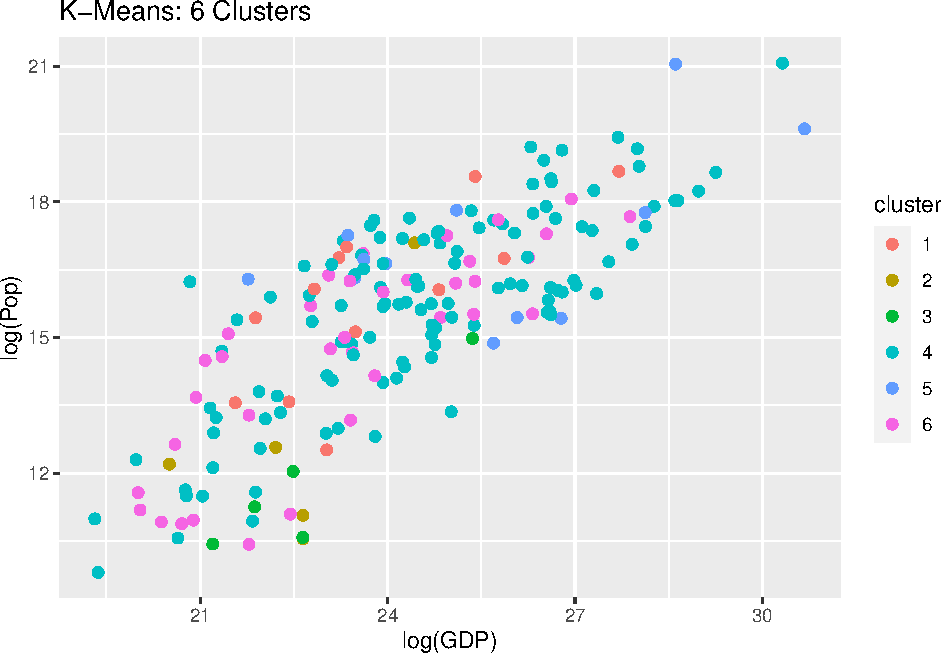
\includegraphics{eda_files/figure-latex/unnamed-chunk-26-1.pdf}

\begin{Shaded}
\begin{Highlighting}[]
\NormalTok{p2 <-}\StringTok{ }\KeywordTok{ggplot}\NormalTok{(master_df_k, }\KeywordTok{aes}\NormalTok{(}\DataTypeTok{x =} \KeywordTok{log}\NormalTok{(GDP), }\DataTypeTok{y =} \KeywordTok{log}\NormalTok{(Expectancy), }\DataTypeTok{color =}\NormalTok{ cluster)) }\OperatorTok{+}
\StringTok{  }\KeywordTok{geom_point}\NormalTok{(}\DataTypeTok{size=}\DecValTok{2}\NormalTok{)}
\NormalTok{p2 }\OperatorTok{+}\StringTok{ }\KeywordTok{ggtitle}\NormalTok{(}\StringTok{"K-Means: 6 Clusters"}\NormalTok{) }\OperatorTok{+}\StringTok{ }\KeywordTok{scale_fill_brewer}\NormalTok{(}\DataTypeTok{palette=}\StringTok{"Set3"}\NormalTok{)}
\end{Highlighting}
\end{Shaded}

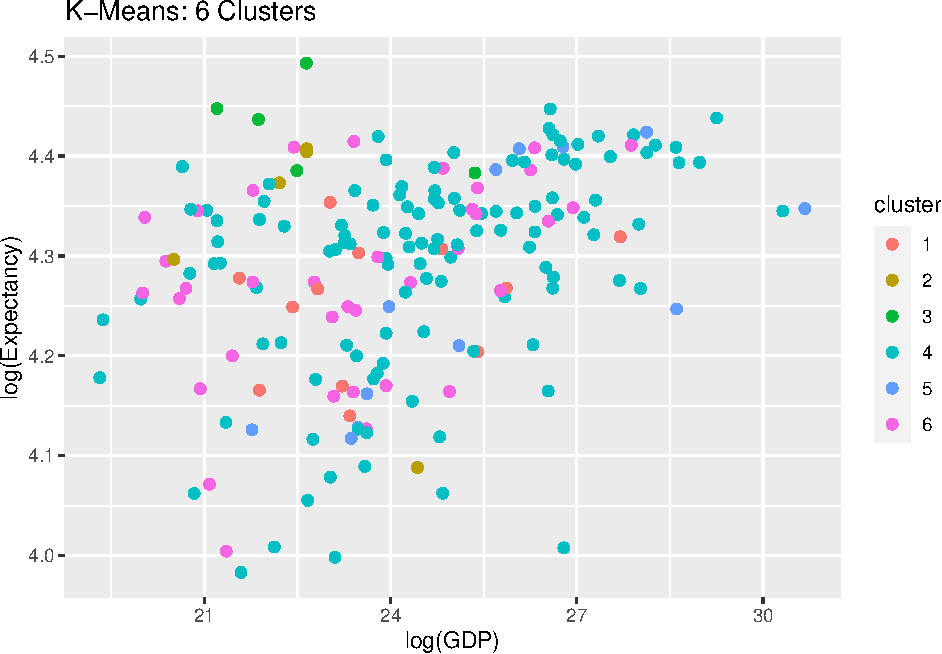
\includegraphics{eda_files/figure-latex/unnamed-chunk-26-2.pdf}

\begin{Shaded}
\begin{Highlighting}[]
\KeywordTok{jpeg}\NormalTok{(}\StringTok{"k_twoway.jpeg"}\NormalTok{)}
\NormalTok{p2 <-}\StringTok{ }\KeywordTok{ggplot}\NormalTok{(master_df_k, }\KeywordTok{aes}\NormalTok{(}\DataTypeTok{x =} \KeywordTok{log}\NormalTok{(GDP), }\DataTypeTok{y =} \KeywordTok{log}\NormalTok{(Fertility), }\DataTypeTok{color =}\NormalTok{ cluster)) }\OperatorTok{+}
\StringTok{  }\KeywordTok{geom_point}\NormalTok{(}\DataTypeTok{size=}\DecValTok{2}\NormalTok{)}
\NormalTok{p2 }\OperatorTok{+}\StringTok{ }\KeywordTok{ggtitle}\NormalTok{(}\StringTok{"K-Means: 6 Clusters"}\NormalTok{) }\OperatorTok{+}\StringTok{ }\KeywordTok{scale_fill_brewer}\NormalTok{(}\DataTypeTok{palette=}\StringTok{"Set3"}\NormalTok{)}
\KeywordTok{dev.off}\NormalTok{()}
\end{Highlighting}
\end{Shaded}

\begin{verbatim}
## pdf 
##   2
\end{verbatim}

\begin{Shaded}
\begin{Highlighting}[]
\NormalTok{p2 <-}\StringTok{ }\KeywordTok{ggplot}\NormalTok{(master_df_k, }\KeywordTok{aes}\NormalTok{(}\DataTypeTok{x =} \KeywordTok{log}\NormalTok{(GDP), }\DataTypeTok{y =} \KeywordTok{log}\NormalTok{(literacy), }\DataTypeTok{color =}\NormalTok{ cluster)) }\OperatorTok{+}
\StringTok{  }\KeywordTok{geom_point}\NormalTok{(}\DataTypeTok{size=}\DecValTok{2}\NormalTok{)}
\NormalTok{p2 }\OperatorTok{+}\StringTok{ }\KeywordTok{ggtitle}\NormalTok{(}\StringTok{"K-Means: 6 Clusters"}\NormalTok{) }\OperatorTok{+}\StringTok{ }\KeywordTok{scale_fill_brewer}\NormalTok{(}\DataTypeTok{palette=}\StringTok{"Set3"}\NormalTok{)}
\end{Highlighting}
\end{Shaded}

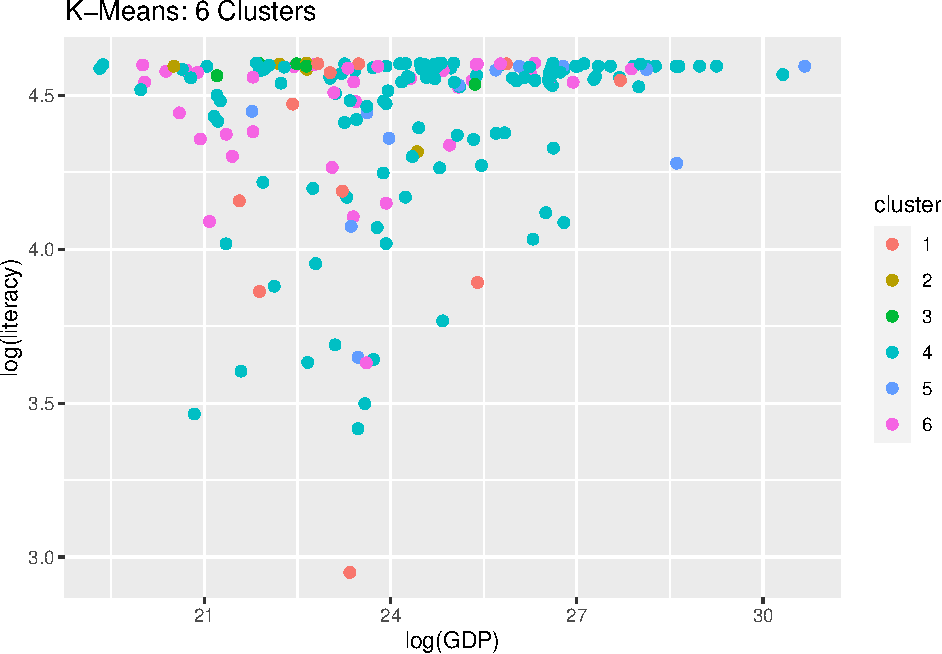
\includegraphics{eda_files/figure-latex/unnamed-chunk-26-3.pdf}

\begin{Shaded}
\begin{Highlighting}[]
\NormalTok{p2 <-}\StringTok{ }\KeywordTok{ggplot}\NormalTok{(master_df_k, }\KeywordTok{aes}\NormalTok{(}\DataTypeTok{x =} \KeywordTok{log}\NormalTok{(GDP), }\DataTypeTok{y =} \KeywordTok{log}\NormalTok{(Expectancy), }\DataTypeTok{color =}\NormalTok{ cluster)) }\OperatorTok{+}
\StringTok{  }\KeywordTok{geom_point}\NormalTok{(}\DataTypeTok{size=}\DecValTok{2}\NormalTok{)}
\NormalTok{p2 }\OperatorTok{+}\StringTok{ }\KeywordTok{ggtitle}\NormalTok{(}\StringTok{"K-Means: 6 Clusters"}\NormalTok{) }\OperatorTok{+}\StringTok{ }\KeywordTok{scale_fill_brewer}\NormalTok{(}\DataTypeTok{palette=}\StringTok{"Set3"}\NormalTok{)}
\end{Highlighting}
\end{Shaded}

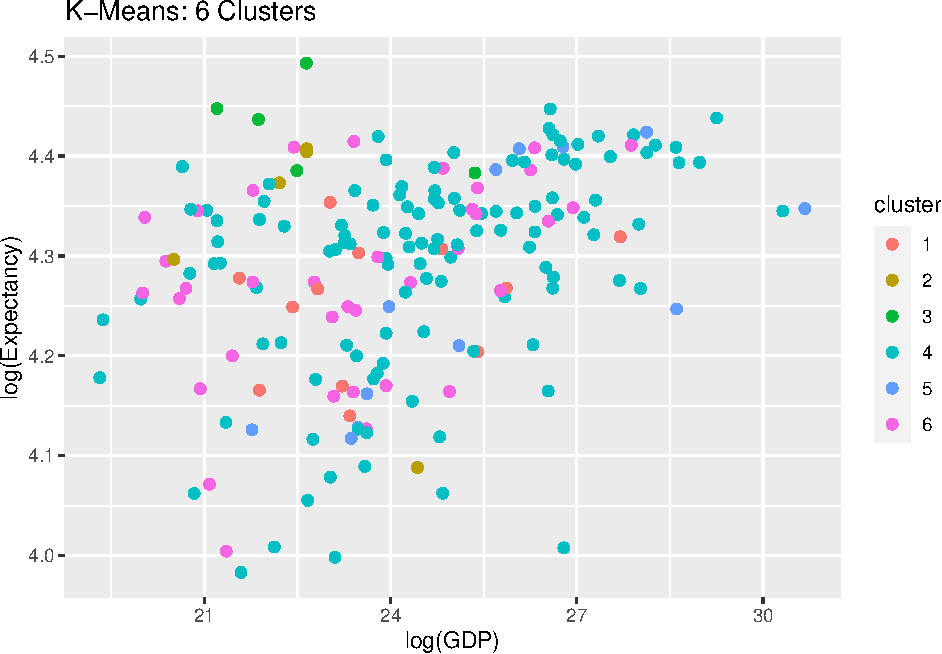
\includegraphics{eda_files/figure-latex/unnamed-chunk-26-4.pdf}

\begin{Shaded}
\begin{Highlighting}[]
\NormalTok{p2 <-}\StringTok{ }\KeywordTok{ggplot}\NormalTok{(master_df_k, }\KeywordTok{aes}\NormalTok{(}\DataTypeTok{x =} \KeywordTok{log}\NormalTok{(Pop), }\DataTypeTok{y =} \KeywordTok{log}\NormalTok{(Expectancy), }\DataTypeTok{color =}\NormalTok{ cluster)) }\OperatorTok{+}
\StringTok{  }\KeywordTok{geom_point}\NormalTok{(}\DataTypeTok{size=}\DecValTok{2}\NormalTok{)}
\NormalTok{p2 }\OperatorTok{+}\StringTok{ }\KeywordTok{ggtitle}\NormalTok{(}\StringTok{"K-Means: 6 Clusters"}\NormalTok{) }\OperatorTok{+}\StringTok{ }\KeywordTok{scale_fill_brewer}\NormalTok{(}\DataTypeTok{palette=}\StringTok{"Set3"}\NormalTok{)}
\end{Highlighting}
\end{Shaded}

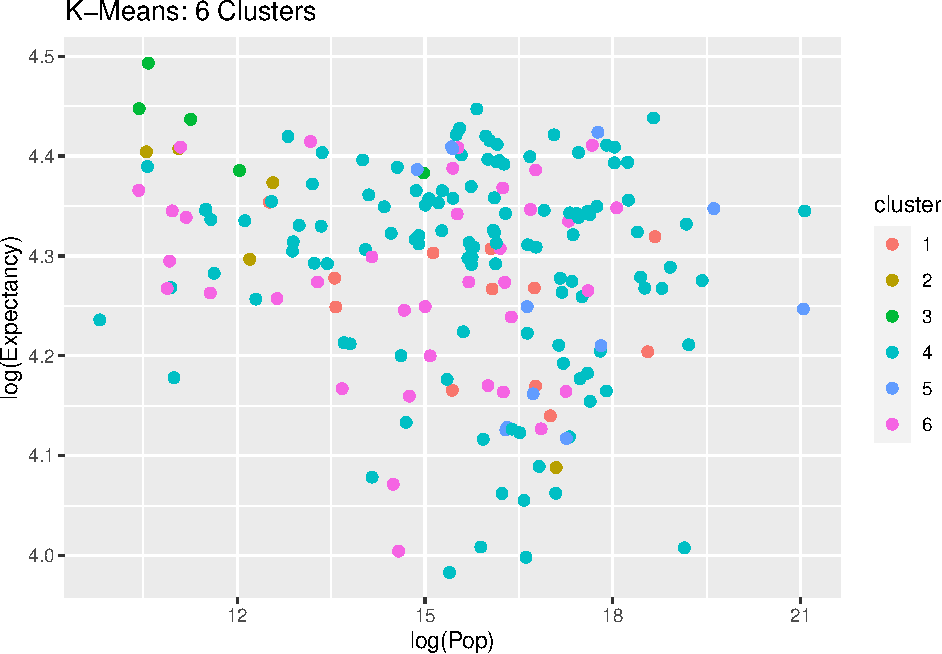
\includegraphics{eda_files/figure-latex/unnamed-chunk-26-5.pdf}

\begin{Shaded}
\begin{Highlighting}[]
\NormalTok{p2 <-}\StringTok{ }\KeywordTok{ggplot}\NormalTok{(master_df_k, }\KeywordTok{aes}\NormalTok{(}\DataTypeTok{x =} \KeywordTok{log}\NormalTok{(Pop), }\DataTypeTok{y =} \KeywordTok{log}\NormalTok{(Fertility), }\DataTypeTok{color =}\NormalTok{ cluster)) }\OperatorTok{+}
\StringTok{  }\KeywordTok{geom_point}\NormalTok{(}\DataTypeTok{size=}\DecValTok{2}\NormalTok{)}
\NormalTok{p2 }\OperatorTok{+}\StringTok{ }\KeywordTok{ggtitle}\NormalTok{(}\StringTok{"K-Means: 6 Clusters"}\NormalTok{) }\OperatorTok{+}\StringTok{ }\KeywordTok{scale_fill_brewer}\NormalTok{(}\DataTypeTok{palette=}\StringTok{"Set3"}\NormalTok{)}
\end{Highlighting}
\end{Shaded}

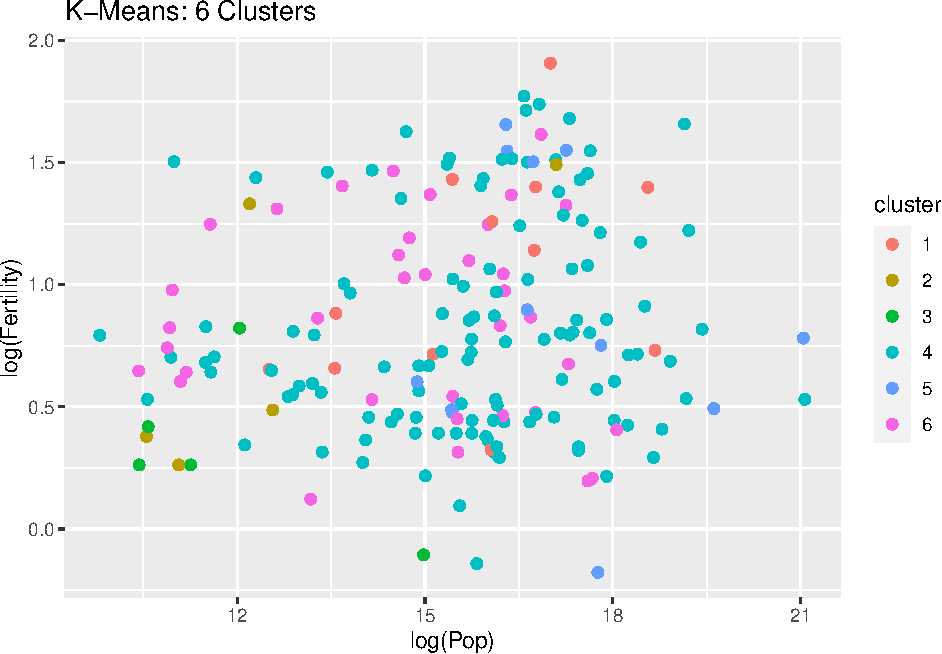
\includegraphics{eda_files/figure-latex/unnamed-chunk-26-6.pdf}

\begin{Shaded}
\begin{Highlighting}[]
\NormalTok{p2 <-}\StringTok{ }\KeywordTok{ggplot}\NormalTok{(master_df_k, }\KeywordTok{aes}\NormalTok{(}\DataTypeTok{x =} \KeywordTok{log}\NormalTok{(Pop), }\DataTypeTok{y =} \KeywordTok{log}\NormalTok{(literacy), }\DataTypeTok{color =}\NormalTok{ cluster)) }\OperatorTok{+}
\StringTok{  }\KeywordTok{geom_point}\NormalTok{(}\DataTypeTok{size=}\DecValTok{2}\NormalTok{)}
\NormalTok{p2 }\OperatorTok{+}\StringTok{ }\KeywordTok{ggtitle}\NormalTok{(}\StringTok{"K-Means: 6 Clusters"}\NormalTok{) }\OperatorTok{+}\StringTok{ }\KeywordTok{scale_fill_brewer}\NormalTok{(}\DataTypeTok{palette=}\StringTok{"Set3"}\NormalTok{)}
\end{Highlighting}
\end{Shaded}

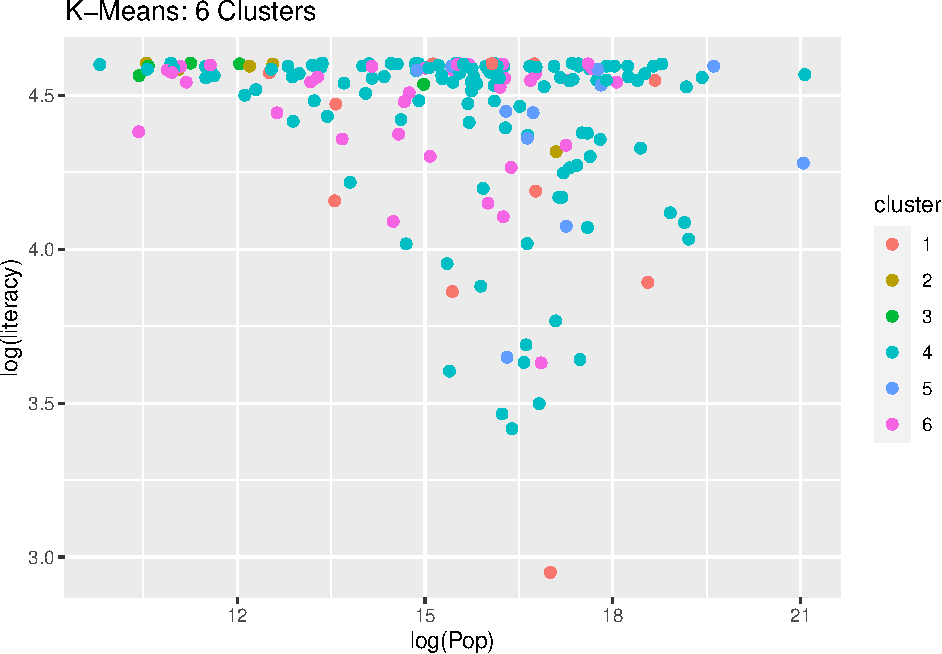
\includegraphics{eda_files/figure-latex/unnamed-chunk-26-7.pdf}

\begin{Shaded}
\begin{Highlighting}[]
\NormalTok{p2 <-}\StringTok{ }\KeywordTok{ggplot}\NormalTok{(master_df_k, }\KeywordTok{aes}\NormalTok{(}\DataTypeTok{x =} \KeywordTok{log}\NormalTok{(Expectancy), }\DataTypeTok{y =} \KeywordTok{log}\NormalTok{(Fertility), }\DataTypeTok{color =}\NormalTok{ cluster)) }\OperatorTok{+}
\StringTok{  }\KeywordTok{geom_point}\NormalTok{(}\DataTypeTok{size=}\DecValTok{2}\NormalTok{)}
\NormalTok{p2 }\OperatorTok{+}\StringTok{ }\KeywordTok{ggtitle}\NormalTok{(}\StringTok{"K-Means: 6 Clusters"}\NormalTok{) }\OperatorTok{+}\StringTok{ }\KeywordTok{scale_fill_brewer}\NormalTok{(}\DataTypeTok{palette=}\StringTok{"Set3"}\NormalTok{)}
\end{Highlighting}
\end{Shaded}

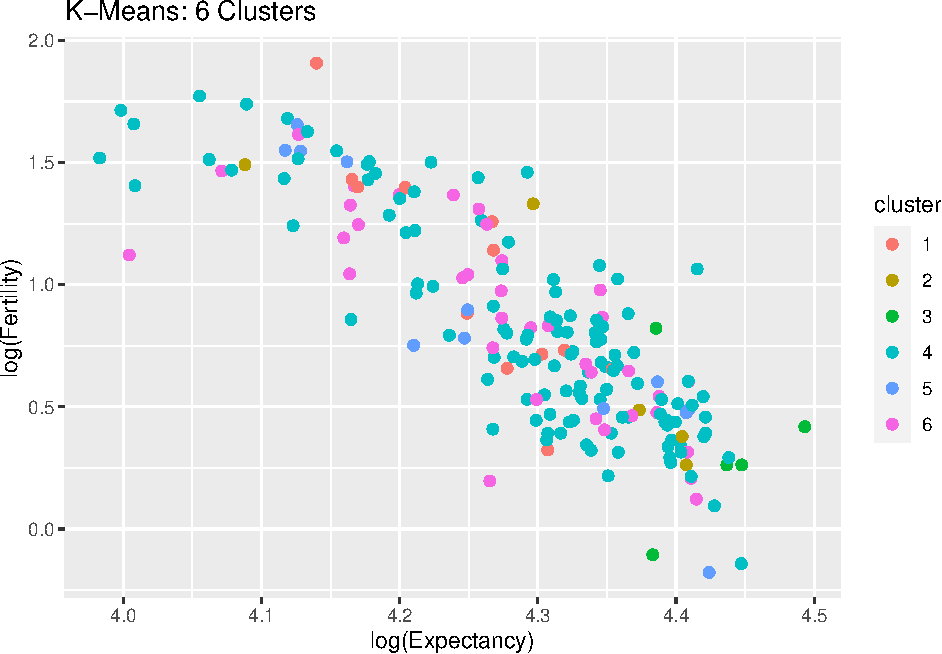
\includegraphics{eda_files/figure-latex/unnamed-chunk-26-8.pdf}

\begin{Shaded}
\begin{Highlighting}[]
\NormalTok{p2 <-}\StringTok{ }\KeywordTok{ggplot}\NormalTok{(master_df_k, }\KeywordTok{aes}\NormalTok{(}\DataTypeTok{x =} \KeywordTok{log}\NormalTok{(Fertility), }\DataTypeTok{y =} \KeywordTok{log}\NormalTok{(literacy), }\DataTypeTok{color =}\NormalTok{ cluster)) }\OperatorTok{+}
\StringTok{  }\KeywordTok{geom_point}\NormalTok{(}\DataTypeTok{size=}\DecValTok{2}\NormalTok{)}
\NormalTok{p2 }\OperatorTok{+}\StringTok{ }\KeywordTok{ggtitle}\NormalTok{(}\StringTok{"K-Means: 6 Clusters"}\NormalTok{) }\OperatorTok{+}\StringTok{ }\KeywordTok{scale_fill_brewer}\NormalTok{(}\DataTypeTok{palette=}\StringTok{"Set3"}\NormalTok{)}
\end{Highlighting}
\end{Shaded}

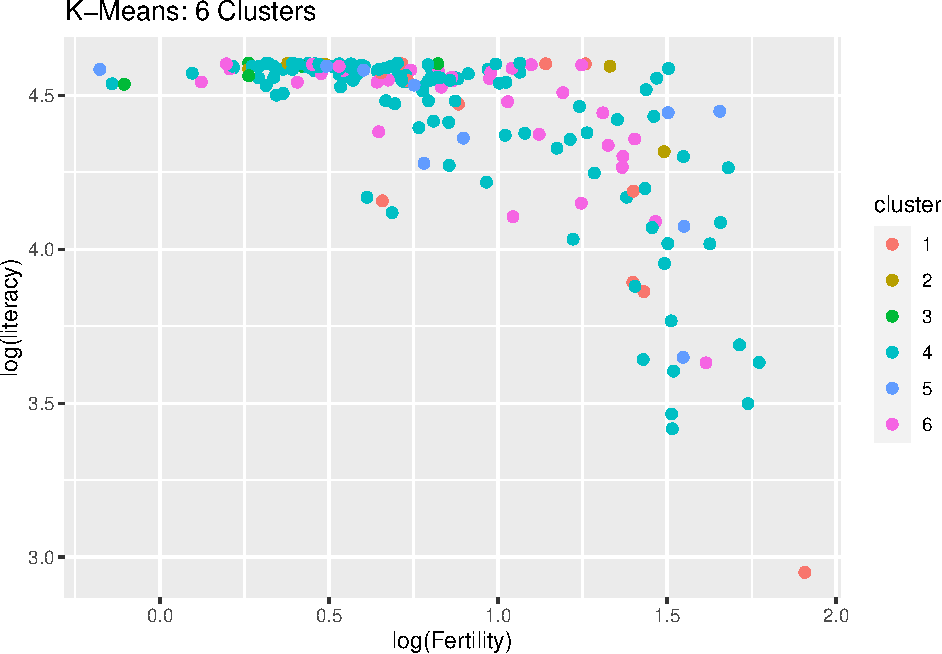
\includegraphics{eda_files/figure-latex/unnamed-chunk-26-9.pdf}

\begin{Shaded}
\begin{Highlighting}[]
\CommentTok{#jpeg(file="kmeans_6.jpg")}
\CommentTok{#dev.off()}

\CommentTok{#jpeg(file="hac_6.jpg")}
\CommentTok{# p3 <- ggplot(master_df_h, aes(x = log(Pop), y = log(Expectancy), color = cluster)) + geom_point(size=2) }
\CommentTok{# p3 + ggtitle("HAC: 6 Clusters") + scale_fill_brewer(palette="Set3")}
\CommentTok{#dev.off()}
\end{Highlighting}
\end{Shaded}

\begin{Shaded}
\begin{Highlighting}[]
\NormalTok{p2 <-}\StringTok{ }\KeywordTok{ggplot}\NormalTok{(master_df_h, }\KeywordTok{aes}\NormalTok{(}\DataTypeTok{x =} \KeywordTok{log}\NormalTok{(GDP), }\DataTypeTok{y =} \KeywordTok{log}\NormalTok{(Pop), }\DataTypeTok{color =}\NormalTok{ cluster)) }\OperatorTok{+}
\StringTok{  }\KeywordTok{geom_point}\NormalTok{(}\DataTypeTok{size=}\DecValTok{2}\NormalTok{)}
\NormalTok{p2 }\OperatorTok{+}\StringTok{ }\KeywordTok{ggtitle}\NormalTok{(}\StringTok{"HAC: 6 Clusters"}\NormalTok{) }\OperatorTok{+}\StringTok{ }\KeywordTok{scale_fill_brewer}\NormalTok{(}\DataTypeTok{palette=}\StringTok{"Set3"}\NormalTok{)}
\end{Highlighting}
\end{Shaded}

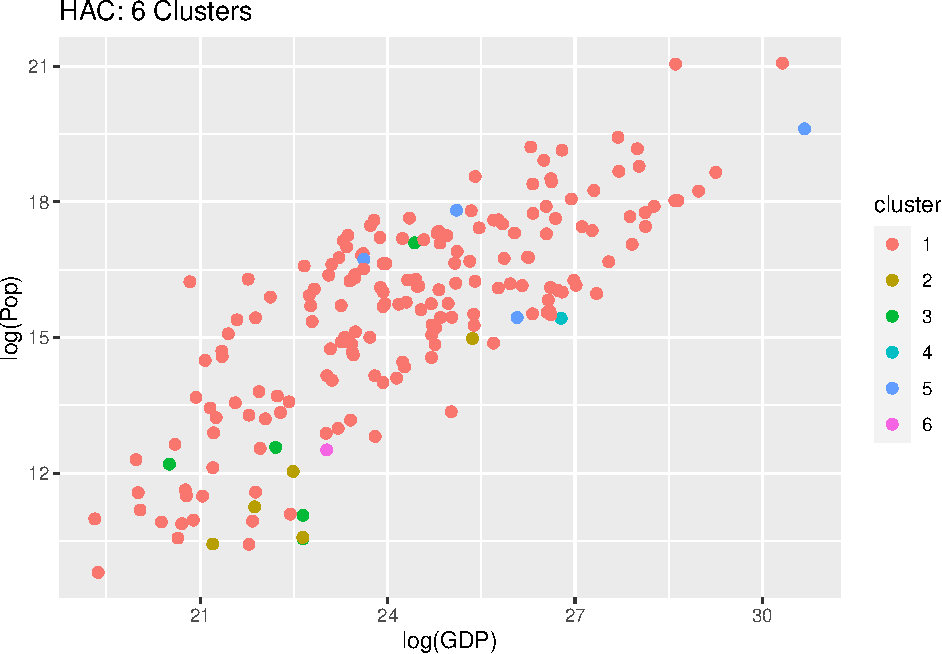
\includegraphics{eda_files/figure-latex/unnamed-chunk-27-1.pdf}

\begin{Shaded}
\begin{Highlighting}[]
\NormalTok{p2 <-}\StringTok{ }\KeywordTok{ggplot}\NormalTok{(master_df_h, }\KeywordTok{aes}\NormalTok{(}\DataTypeTok{x =} \KeywordTok{log}\NormalTok{(GDP), }\DataTypeTok{y =} \KeywordTok{log}\NormalTok{(Expectancy), }\DataTypeTok{color =}\NormalTok{ cluster)) }\OperatorTok{+}
\StringTok{  }\KeywordTok{geom_point}\NormalTok{(}\DataTypeTok{size=}\DecValTok{2}\NormalTok{)}
\NormalTok{p2 }\OperatorTok{+}\StringTok{ }\KeywordTok{ggtitle}\NormalTok{(}\StringTok{"HAC: 6 Clusters"}\NormalTok{) }\OperatorTok{+}\StringTok{ }\KeywordTok{scale_fill_brewer}\NormalTok{(}\DataTypeTok{palette=}\StringTok{"Set3"}\NormalTok{)}
\end{Highlighting}
\end{Shaded}

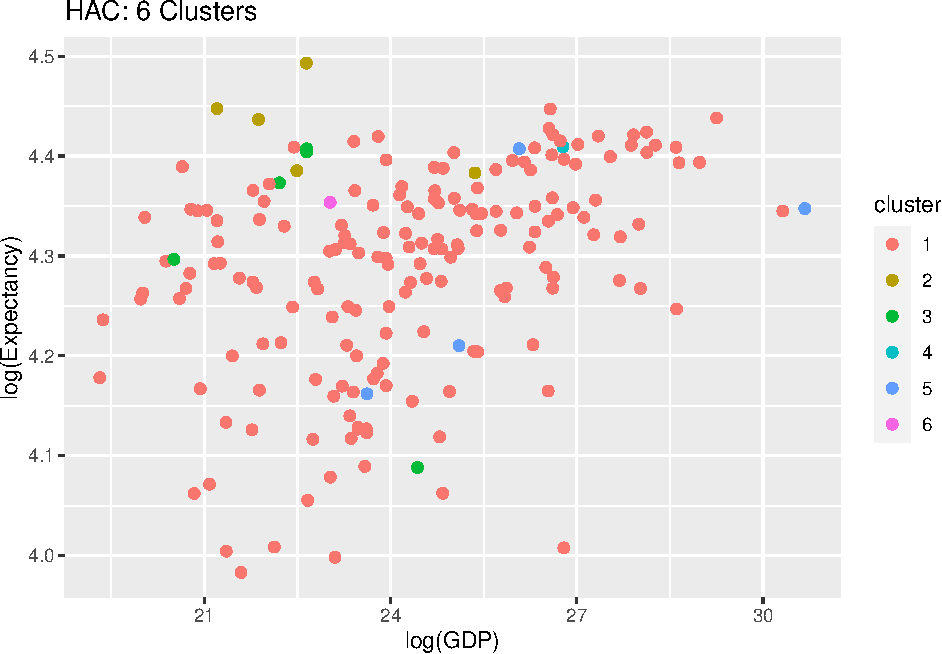
\includegraphics{eda_files/figure-latex/unnamed-chunk-27-2.pdf}

\begin{Shaded}
\begin{Highlighting}[]
\NormalTok{p2 <-}\StringTok{ }\KeywordTok{ggplot}\NormalTok{(master_df_h, }\KeywordTok{aes}\NormalTok{(}\DataTypeTok{x =} \KeywordTok{log}\NormalTok{(GDP), }\DataTypeTok{y =} \KeywordTok{log}\NormalTok{(Fertility), }\DataTypeTok{color =}\NormalTok{ cluster)) }\OperatorTok{+}
\StringTok{  }\KeywordTok{geom_point}\NormalTok{(}\DataTypeTok{size=}\DecValTok{2}\NormalTok{)}
\NormalTok{p2 }\OperatorTok{+}\StringTok{ }\KeywordTok{ggtitle}\NormalTok{(}\StringTok{"HAC: 6 Clusters"}\NormalTok{) }\OperatorTok{+}\StringTok{ }\KeywordTok{scale_fill_brewer}\NormalTok{(}\DataTypeTok{palette=}\StringTok{"Set3"}\NormalTok{)}
\end{Highlighting}
\end{Shaded}

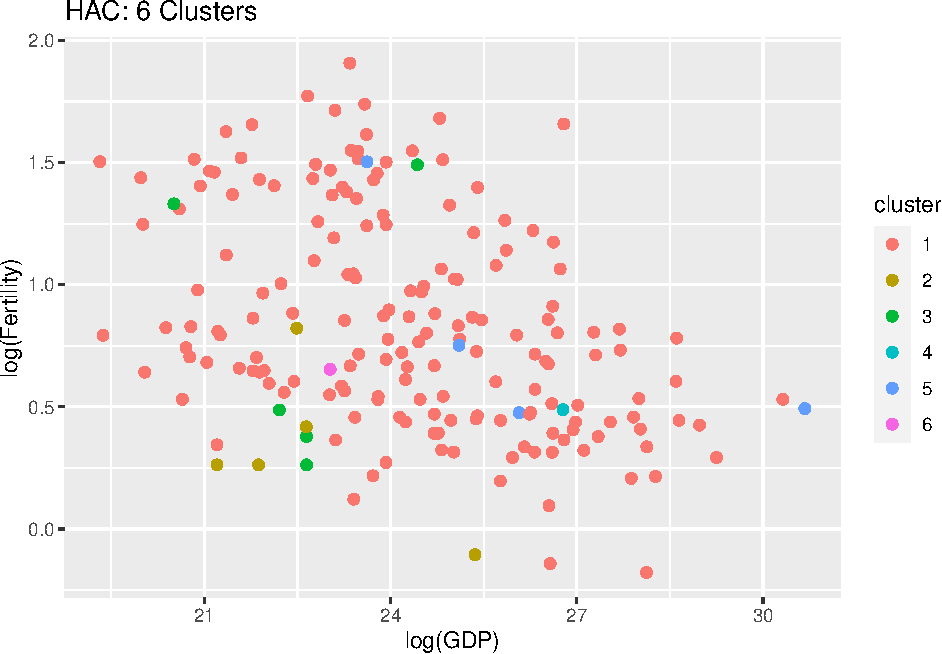
\includegraphics{eda_files/figure-latex/unnamed-chunk-27-3.pdf}

\begin{Shaded}
\begin{Highlighting}[]
\NormalTok{p2 <-}\StringTok{ }\KeywordTok{ggplot}\NormalTok{(master_df_h, }\KeywordTok{aes}\NormalTok{(}\DataTypeTok{x =} \KeywordTok{log}\NormalTok{(GDP), }\DataTypeTok{y =} \KeywordTok{log}\NormalTok{(literacy), }\DataTypeTok{color =}\NormalTok{ cluster)) }\OperatorTok{+}
\StringTok{  }\KeywordTok{geom_point}\NormalTok{(}\DataTypeTok{size=}\DecValTok{2}\NormalTok{)}
\NormalTok{p2 }\OperatorTok{+}\StringTok{ }\KeywordTok{ggtitle}\NormalTok{(}\StringTok{"HAC: 6 Clusters"}\NormalTok{) }\OperatorTok{+}\StringTok{ }\KeywordTok{scale_fill_brewer}\NormalTok{(}\DataTypeTok{palette=}\StringTok{"Set3"}\NormalTok{)}
\end{Highlighting}
\end{Shaded}

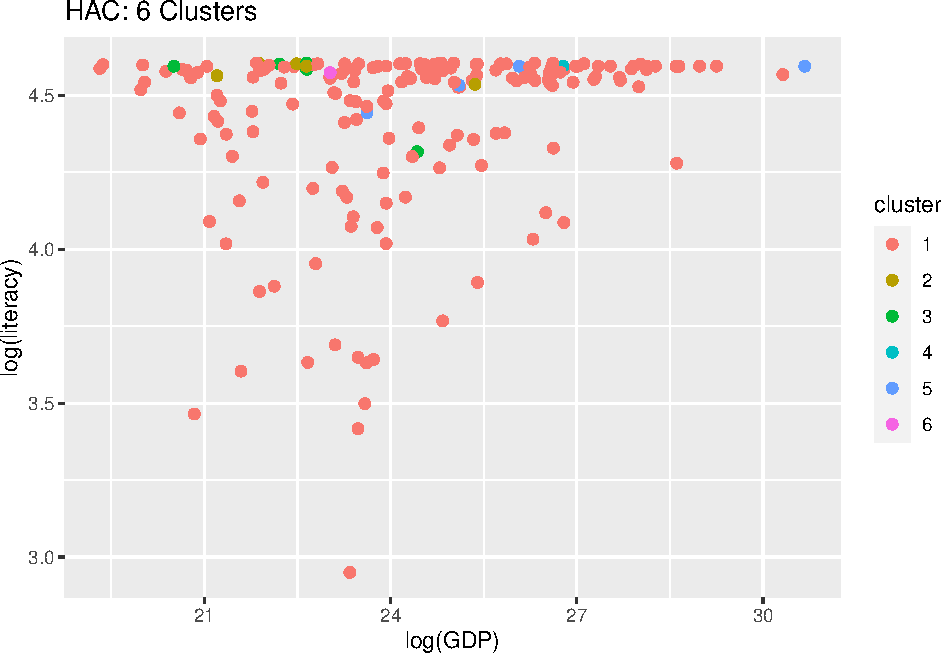
\includegraphics{eda_files/figure-latex/unnamed-chunk-27-4.pdf}

\begin{Shaded}
\begin{Highlighting}[]
\NormalTok{p2 <-}\StringTok{ }\KeywordTok{ggplot}\NormalTok{(master_df_h, }\KeywordTok{aes}\NormalTok{(}\DataTypeTok{x =} \KeywordTok{log}\NormalTok{(GDP), }\DataTypeTok{y =} \KeywordTok{log}\NormalTok{(Expectancy), }\DataTypeTok{color =}\NormalTok{ cluster)) }\OperatorTok{+}
\StringTok{  }\KeywordTok{geom_point}\NormalTok{(}\DataTypeTok{size=}\DecValTok{2}\NormalTok{)}
\NormalTok{p2 }\OperatorTok{+}\StringTok{ }\KeywordTok{ggtitle}\NormalTok{(}\StringTok{"HAC: 6 Clusters"}\NormalTok{) }\OperatorTok{+}\StringTok{ }\KeywordTok{scale_fill_brewer}\NormalTok{(}\DataTypeTok{palette=}\StringTok{"Set3"}\NormalTok{)}
\end{Highlighting}
\end{Shaded}

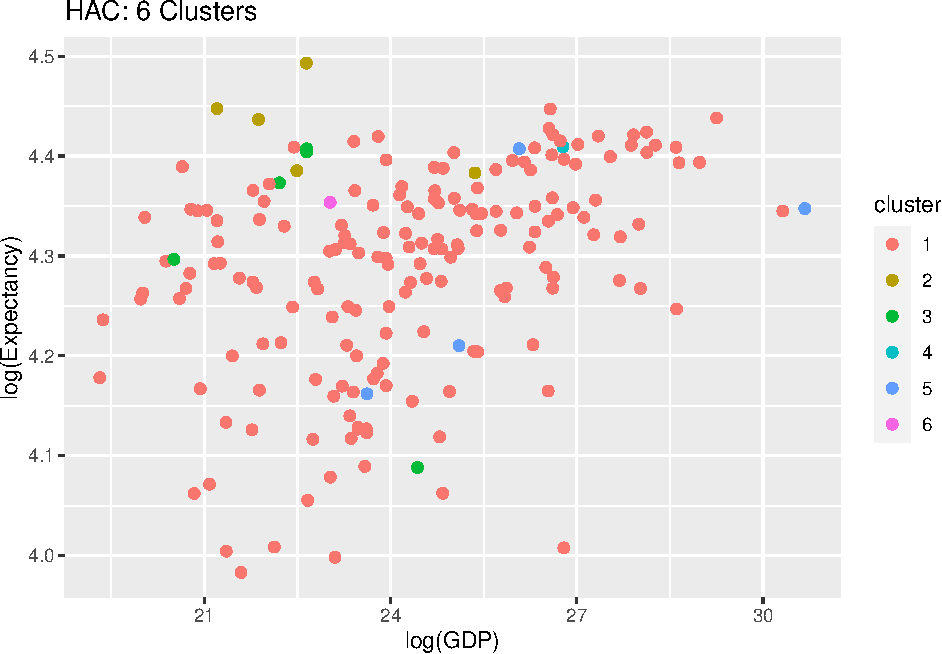
\includegraphics{eda_files/figure-latex/unnamed-chunk-27-5.pdf}

\begin{Shaded}
\begin{Highlighting}[]
\NormalTok{p2 <-}\StringTok{ }\KeywordTok{ggplot}\NormalTok{(master_df_h, }\KeywordTok{aes}\NormalTok{(}\DataTypeTok{x =} \KeywordTok{log}\NormalTok{(Pop), }\DataTypeTok{y =} \KeywordTok{log}\NormalTok{(Expectancy), }\DataTypeTok{color =}\NormalTok{ cluster)) }\OperatorTok{+}
\StringTok{  }\KeywordTok{geom_point}\NormalTok{(}\DataTypeTok{size=}\DecValTok{2}\NormalTok{)}
\NormalTok{p2 }\OperatorTok{+}\StringTok{ }\KeywordTok{ggtitle}\NormalTok{(}\StringTok{"HAC: 6 Clusters"}\NormalTok{) }\OperatorTok{+}\StringTok{ }\KeywordTok{scale_fill_brewer}\NormalTok{(}\DataTypeTok{palette=}\StringTok{"Set3"}\NormalTok{)}
\end{Highlighting}
\end{Shaded}

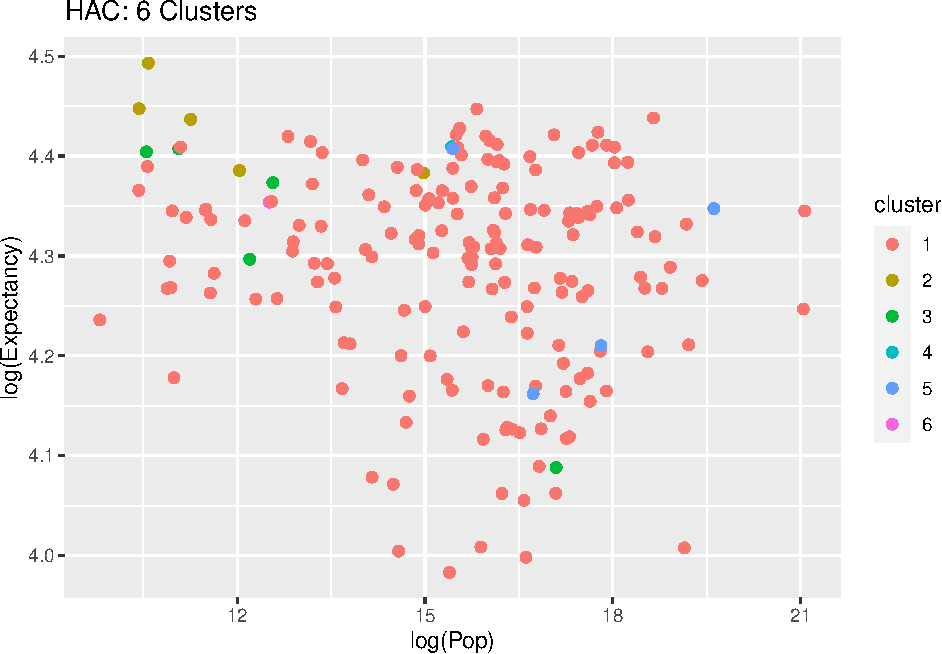
\includegraphics{eda_files/figure-latex/unnamed-chunk-27-6.pdf}

\begin{Shaded}
\begin{Highlighting}[]
\NormalTok{p2 <-}\StringTok{ }\KeywordTok{ggplot}\NormalTok{(master_df_h, }\KeywordTok{aes}\NormalTok{(}\DataTypeTok{x =} \KeywordTok{log}\NormalTok{(Pop), }\DataTypeTok{y =} \KeywordTok{log}\NormalTok{(Fertility), }\DataTypeTok{color =}\NormalTok{ cluster)) }\OperatorTok{+}
\StringTok{  }\KeywordTok{geom_point}\NormalTok{(}\DataTypeTok{size=}\DecValTok{2}\NormalTok{)}
\NormalTok{p2 }\OperatorTok{+}\StringTok{ }\KeywordTok{ggtitle}\NormalTok{(}\StringTok{"HAC: 6 Clusters"}\NormalTok{) }\OperatorTok{+}\StringTok{ }\KeywordTok{scale_fill_brewer}\NormalTok{(}\DataTypeTok{palette=}\StringTok{"Set3"}\NormalTok{)}
\end{Highlighting}
\end{Shaded}

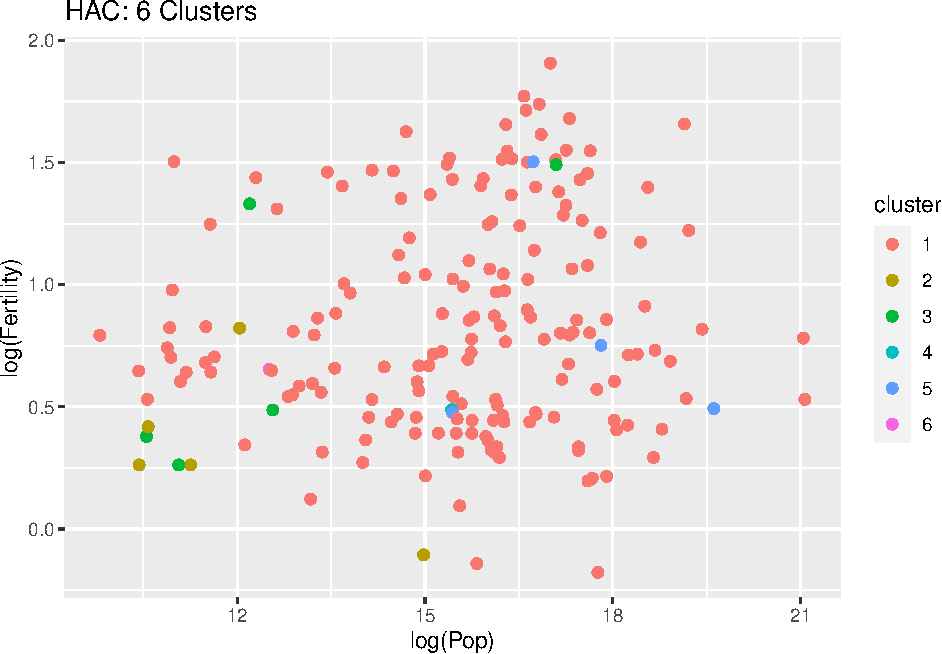
\includegraphics{eda_files/figure-latex/unnamed-chunk-27-7.pdf}

\begin{Shaded}
\begin{Highlighting}[]
\KeywordTok{jpeg}\NormalTok{(}\StringTok{'hac_twoway.jpeg'}\NormalTok{)}
\NormalTok{p2 <-}\StringTok{ }\KeywordTok{ggplot}\NormalTok{(master_df_h, }\KeywordTok{aes}\NormalTok{(}\DataTypeTok{x =} \KeywordTok{log}\NormalTok{(Pop), }\DataTypeTok{y =} \KeywordTok{log}\NormalTok{(literacy), }\DataTypeTok{color =}\NormalTok{ cluster)) }\OperatorTok{+}
\StringTok{  }\KeywordTok{geom_point}\NormalTok{(}\DataTypeTok{size=}\DecValTok{2}\NormalTok{)}
\NormalTok{p2 }\OperatorTok{+}\StringTok{ }\KeywordTok{ggtitle}\NormalTok{(}\StringTok{"HAC: 6 Clusters"}\NormalTok{) }\OperatorTok{+}\StringTok{ }\KeywordTok{scale_fill_brewer}\NormalTok{(}\DataTypeTok{palette=}\StringTok{"Set3"}\NormalTok{)}
\KeywordTok{dev.off}\NormalTok{()}
\end{Highlighting}
\end{Shaded}

\begin{verbatim}
## pdf 
##   2
\end{verbatim}

\begin{Shaded}
\begin{Highlighting}[]
\NormalTok{p2 <-}\StringTok{ }\KeywordTok{ggplot}\NormalTok{(master_df_h, }\KeywordTok{aes}\NormalTok{(}\DataTypeTok{x =} \KeywordTok{log}\NormalTok{(Expectancy), }\DataTypeTok{y =} \KeywordTok{log}\NormalTok{(Fertility), }\DataTypeTok{color =}\NormalTok{ cluster)) }\OperatorTok{+}
\StringTok{  }\KeywordTok{geom_point}\NormalTok{(}\DataTypeTok{size=}\DecValTok{2}\NormalTok{)}
\NormalTok{p2 }\OperatorTok{+}\StringTok{ }\KeywordTok{ggtitle}\NormalTok{(}\StringTok{"HAC: 6 Clusters"}\NormalTok{) }\OperatorTok{+}\StringTok{ }\KeywordTok{scale_fill_brewer}\NormalTok{(}\DataTypeTok{palette=}\StringTok{"Set3"}\NormalTok{)}
\end{Highlighting}
\end{Shaded}

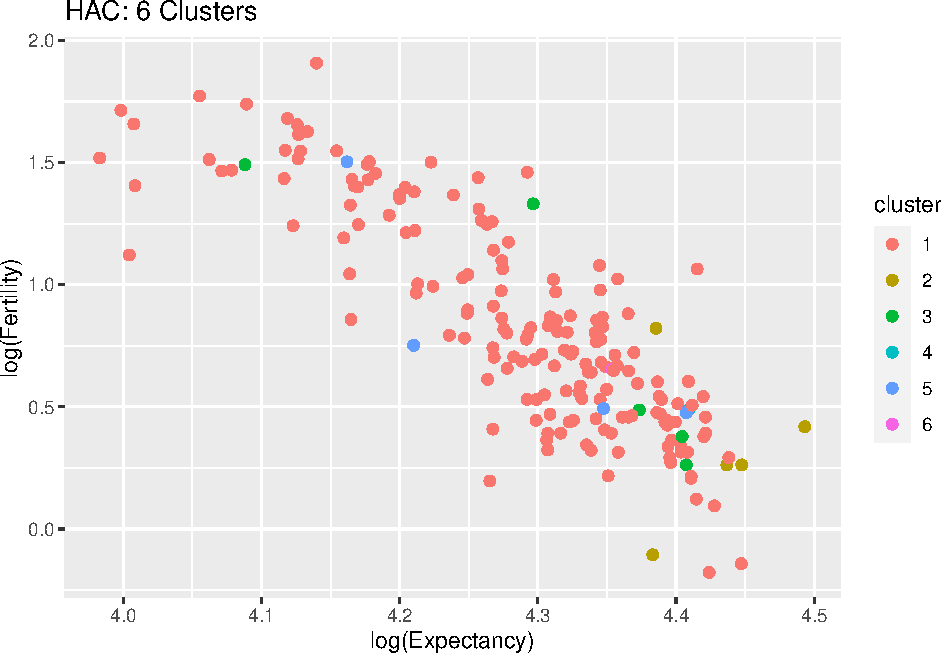
\includegraphics{eda_files/figure-latex/unnamed-chunk-27-8.pdf}

\begin{Shaded}
\begin{Highlighting}[]
\NormalTok{p2 <-}\StringTok{ }\KeywordTok{ggplot}\NormalTok{(master_df_h, }\KeywordTok{aes}\NormalTok{(}\DataTypeTok{x =} \KeywordTok{log}\NormalTok{(Fertility), }\DataTypeTok{y =} \KeywordTok{log}\NormalTok{(literacy), }\DataTypeTok{color =}\NormalTok{ cluster)) }\OperatorTok{+}
\StringTok{  }\KeywordTok{geom_point}\NormalTok{(}\DataTypeTok{size=}\DecValTok{2}\NormalTok{)}
\NormalTok{p2 }\OperatorTok{+}\StringTok{ }\KeywordTok{ggtitle}\NormalTok{(}\StringTok{"HAC: 6 Clusters"}\NormalTok{) }\OperatorTok{+}\StringTok{ }\KeywordTok{scale_fill_brewer}\NormalTok{(}\DataTypeTok{palette=}\StringTok{"Set3"}\NormalTok{)}
\end{Highlighting}
\end{Shaded}

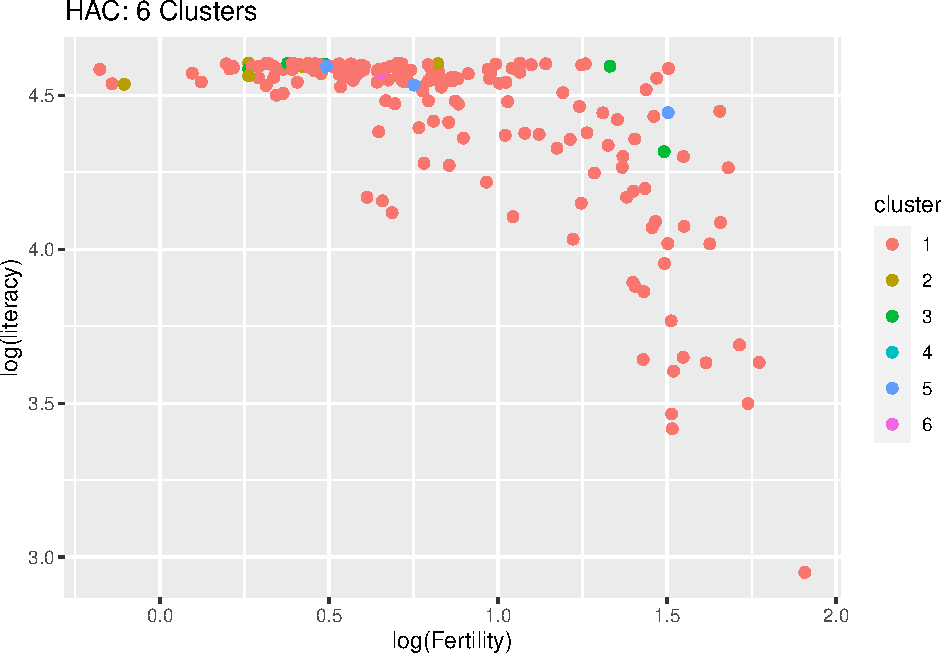
\includegraphics{eda_files/figure-latex/unnamed-chunk-27-9.pdf}

\begin{Shaded}
\begin{Highlighting}[]
\CommentTok{# manually label outliers for boxplots}

\NormalTok{master_df_k}\OperatorTok{$}\NormalTok{outlier_expectancy <-}\StringTok{ }\KeywordTok{rep}\NormalTok{(}\DecValTok{0}\NormalTok{, }\KeywordTok{nrow}\NormalTok{(master_df_k))}
\ControlFlowTok{for}\NormalTok{ (i }\ControlFlowTok{in} \DecValTok{1}\OperatorTok{:}\DecValTok{10}\NormalTok{) \{}
\NormalTok{  med =}\StringTok{ }\KeywordTok{median}\NormalTok{(master_df_k[master_df_k}\OperatorTok{$}\NormalTok{cluster }\OperatorTok{==}\StringTok{ }\NormalTok{i, ]}\OperatorTok{$}\NormalTok{Expectancy)}
\NormalTok{  iqr =}\StringTok{ }\KeywordTok{IQR}\NormalTok{(master_df_k[master_df_k}\OperatorTok{$}\NormalTok{cluster }\OperatorTok{==}\StringTok{ }\NormalTok{i, ]}\OperatorTok{$}\NormalTok{Expectancy)}
\NormalTok{  master_df_k[master_df_k}\OperatorTok{$}\NormalTok{cluster }\OperatorTok{==}\StringTok{ }\NormalTok{i, ]}\OperatorTok{$}\NormalTok{outlier_expectancy <-}\StringTok{ }
\StringTok{    }\NormalTok{(master_df_k[master_df_k}\OperatorTok{$}\NormalTok{cluster }\OperatorTok{==}\StringTok{ }\NormalTok{i, ]}\OperatorTok{$}\NormalTok{Expectancy}\OperatorTok{>}\StringTok{ }\NormalTok{med }\OperatorTok{+}\StringTok{ }\FloatTok{1.5} \OperatorTok{*}\StringTok{ }\NormalTok{iqr) }\OperatorTok{|}
\StringTok{    }\NormalTok{(master_df_k[master_df_k}\OperatorTok{$}\NormalTok{cluster }\OperatorTok{==}\StringTok{ }\NormalTok{i, ]}\OperatorTok{$}\NormalTok{Expectancy }\OperatorTok{<}\StringTok{ }\NormalTok{med }\OperatorTok{-}\StringTok{ }\FloatTok{1.5} \OperatorTok{*}\StringTok{ }\NormalTok{iqr)}
\NormalTok{\}}

\NormalTok{master_df_k}\OperatorTok{$}\NormalTok{outlier_gdp <-}\StringTok{ }\KeywordTok{rep}\NormalTok{(}\DecValTok{0}\NormalTok{, }\KeywordTok{nrow}\NormalTok{(master_df_k))}
\ControlFlowTok{for}\NormalTok{ (i }\ControlFlowTok{in} \DecValTok{1}\OperatorTok{:}\DecValTok{10}\NormalTok{) \{}
\NormalTok{  med =}\StringTok{ }\KeywordTok{median}\NormalTok{(}\KeywordTok{log}\NormalTok{(master_df_k[master_df_k}\OperatorTok{$}\NormalTok{cluster }\OperatorTok{==}\StringTok{ }\NormalTok{i, ]}\OperatorTok{$}\NormalTok{GDP))}
\NormalTok{  iqr =}\StringTok{ }\KeywordTok{IQR}\NormalTok{(}\KeywordTok{log}\NormalTok{(master_df_k[master_df_k}\OperatorTok{$}\NormalTok{cluster }\OperatorTok{==}\StringTok{ }\NormalTok{i, ]}\OperatorTok{$}\NormalTok{GDP))}
\NormalTok{  master_df_k[master_df_k}\OperatorTok{$}\NormalTok{cluster }\OperatorTok{==}\StringTok{ }\NormalTok{i, ]}\OperatorTok{$}\NormalTok{outlier_gdp <-}\StringTok{ }
\StringTok{    }\NormalTok{(}\KeywordTok{log}\NormalTok{(master_df_k[master_df_k}\OperatorTok{$}\NormalTok{cluster }\OperatorTok{==}\StringTok{ }\NormalTok{i, ]}\OperatorTok{$}\NormalTok{GDP) }\OperatorTok{>}\StringTok{ }\NormalTok{med }\OperatorTok{+}\StringTok{ }\FloatTok{1.5} \OperatorTok{*}\StringTok{ }\NormalTok{iqr) }\OperatorTok{|}
\StringTok{    }\NormalTok{(}\KeywordTok{log}\NormalTok{(master_df_k[master_df_k}\OperatorTok{$}\NormalTok{cluster }\OperatorTok{==}\StringTok{ }\NormalTok{i, ]}\OperatorTok{$}\NormalTok{GDP) }\OperatorTok{<}\StringTok{ }\NormalTok{med }\OperatorTok{-}\StringTok{ }\FloatTok{1.5} \OperatorTok{*}\StringTok{ }\NormalTok{iqr)}
\NormalTok{\}}
\end{Highlighting}
\end{Shaded}

\begin{Shaded}
\begin{Highlighting}[]
\CommentTok{# outliers for df_h}

\NormalTok{master_df_h}\OperatorTok{$}\NormalTok{outlier_expectancy <-}\StringTok{ }\KeywordTok{rep}\NormalTok{(}\DecValTok{0}\NormalTok{, }\KeywordTok{nrow}\NormalTok{(master_df_h))}
\ControlFlowTok{for}\NormalTok{ (i }\ControlFlowTok{in} \DecValTok{1}\OperatorTok{:}\DecValTok{10}\NormalTok{) \{}
\NormalTok{  med =}\StringTok{ }\KeywordTok{median}\NormalTok{(master_df_k[master_df_h}\OperatorTok{$}\NormalTok{cluster }\OperatorTok{==}\StringTok{ }\NormalTok{i, ]}\OperatorTok{$}\NormalTok{Expectancy)}
\NormalTok{  iqr =}\StringTok{ }\KeywordTok{IQR}\NormalTok{(master_df_k[master_df_h}\OperatorTok{$}\NormalTok{cluster }\OperatorTok{==}\StringTok{ }\NormalTok{i, ]}\OperatorTok{$}\NormalTok{Expectancy)}
\NormalTok{  master_df_h[master_df_h}\OperatorTok{$}\NormalTok{cluster }\OperatorTok{==}\StringTok{ }\NormalTok{i, ]}\OperatorTok{$}\NormalTok{outlier_expectancy <-}\StringTok{ }
\StringTok{    }\NormalTok{(master_df_h[master_df_h}\OperatorTok{$}\NormalTok{cluster }\OperatorTok{==}\StringTok{ }\NormalTok{i, ]}\OperatorTok{$}\NormalTok{Expectancy}\OperatorTok{>}\StringTok{ }\NormalTok{med }\OperatorTok{+}\StringTok{ }\FloatTok{1.5} \OperatorTok{*}\StringTok{ }\NormalTok{iqr) }\OperatorTok{|}
\StringTok{    }\NormalTok{(master_df_h[master_df_h}\OperatorTok{$}\NormalTok{cluster }\OperatorTok{==}\StringTok{ }\NormalTok{i, ]}\OperatorTok{$}\NormalTok{Expectancy }\OperatorTok{<}\StringTok{ }\NormalTok{med }\OperatorTok{-}\StringTok{ }\FloatTok{1.5} \OperatorTok{*}\StringTok{ }\NormalTok{iqr)}
\NormalTok{\}}

\NormalTok{master_df_h}\OperatorTok{$}\NormalTok{outlier_gdp <-}\StringTok{ }\KeywordTok{rep}\NormalTok{(}\DecValTok{0}\NormalTok{, }\KeywordTok{nrow}\NormalTok{(master_df_h))}
\ControlFlowTok{for}\NormalTok{ (i }\ControlFlowTok{in} \DecValTok{1}\OperatorTok{:}\DecValTok{10}\NormalTok{) \{}
\NormalTok{  med =}\StringTok{ }\KeywordTok{median}\NormalTok{(}\KeywordTok{log}\NormalTok{(master_df_h[master_df_h}\OperatorTok{$}\NormalTok{cluster }\OperatorTok{==}\StringTok{ }\NormalTok{i, ]}\OperatorTok{$}\NormalTok{GDP))}
\NormalTok{  iqr =}\StringTok{ }\KeywordTok{IQR}\NormalTok{(}\KeywordTok{log}\NormalTok{(master_df_h[master_df_h}\OperatorTok{$}\NormalTok{cluster }\OperatorTok{==}\StringTok{ }\NormalTok{i, ]}\OperatorTok{$}\NormalTok{GDP))}
\NormalTok{  master_df_h[master_df_h}\OperatorTok{$}\NormalTok{cluster }\OperatorTok{==}\StringTok{ }\NormalTok{i, ]}\OperatorTok{$}\NormalTok{outlier_gdp <-}\StringTok{ }
\StringTok{    }\NormalTok{(}\KeywordTok{log}\NormalTok{(master_df_h[master_df_h}\OperatorTok{$}\NormalTok{cluster }\OperatorTok{==}\StringTok{ }\NormalTok{i, ]}\OperatorTok{$}\NormalTok{GDP) }\OperatorTok{>}\StringTok{ }\NormalTok{med }\OperatorTok{+}\StringTok{ }\FloatTok{1.5} \OperatorTok{*}\StringTok{ }\NormalTok{iqr) }\OperatorTok{|}
\StringTok{    }\NormalTok{(}\KeywordTok{log}\NormalTok{(master_df_h[master_df_h}\OperatorTok{$}\NormalTok{cluster }\OperatorTok{==}\StringTok{ }\NormalTok{i, ]}\OperatorTok{$}\NormalTok{GDP) }\OperatorTok{<}\StringTok{ }\NormalTok{med }\OperatorTok{-}\StringTok{ }\FloatTok{1.5} \OperatorTok{*}\StringTok{ }\NormalTok{iqr)}
\NormalTok{\}}

\CommentTok{# for NON-significant test result}

\NormalTok{master_df_h}\OperatorTok{$}\NormalTok{outlier_literacy <-}\StringTok{ }\KeywordTok{rep}\NormalTok{(}\DecValTok{0}\NormalTok{, }\KeywordTok{nrow}\NormalTok{(master_df_h))}
\ControlFlowTok{for}\NormalTok{ (i }\ControlFlowTok{in} \DecValTok{1}\OperatorTok{:}\DecValTok{10}\NormalTok{) \{}
\NormalTok{  med =}\StringTok{ }\KeywordTok{median}\NormalTok{(master_df_h[master_df_h}\OperatorTok{$}\NormalTok{cluster }\OperatorTok{==}\StringTok{ }\NormalTok{i, ]}\OperatorTok{$}\NormalTok{literacy)}
\NormalTok{  iqr =}\StringTok{ }\KeywordTok{IQR}\NormalTok{(master_df_h[master_df_h}\OperatorTok{$}\NormalTok{cluster }\OperatorTok{==}\StringTok{ }\NormalTok{i, ]}\OperatorTok{$}\NormalTok{literacy)}
\NormalTok{  master_df_h[master_df_h}\OperatorTok{$}\NormalTok{cluster }\OperatorTok{==}\StringTok{ }\NormalTok{i, ]}\OperatorTok{$}\NormalTok{outlier_literacy <-}\StringTok{ }
\StringTok{    }\NormalTok{(master_df_h[master_df_h}\OperatorTok{$}\NormalTok{cluster }\OperatorTok{==}\StringTok{ }\NormalTok{i, ]}\OperatorTok{$}\NormalTok{literacy }\OperatorTok{>}\StringTok{ }\NormalTok{med }\OperatorTok{+}\StringTok{ }\FloatTok{1.5} \OperatorTok{*}\StringTok{ }\NormalTok{iqr) }\OperatorTok{|}
\StringTok{    }\NormalTok{(master_df_h[master_df_h}\OperatorTok{$}\NormalTok{cluster }\OperatorTok{==}\StringTok{ }\NormalTok{i, ]}\OperatorTok{$}\NormalTok{literacy }\OperatorTok{<}\StringTok{ }\NormalTok{med }\OperatorTok{-}\StringTok{ }\FloatTok{1.5} \OperatorTok{*}\StringTok{ }\NormalTok{iqr)}
\NormalTok{\}}
\end{Highlighting}
\end{Shaded}

\begin{Shaded}
\begin{Highlighting}[]
\CommentTok{# non-significant test result}
\KeywordTok{jpeg}\NormalTok{(}\DataTypeTok{file=}\StringTok{"boxplot_h_literacy.jpg"}\NormalTok{)}
\CommentTok{# do this manually}
\KeywordTok{ggplot}\NormalTok{(master_df_h, }\KeywordTok{aes}\NormalTok{(}\DataTypeTok{x =}\NormalTok{ cluster, }\DataTypeTok{y =}\NormalTok{ literacy, }\DataTypeTok{fill =}\NormalTok{ cluster)) }\OperatorTok{+}
\StringTok{  }\KeywordTok{geom_boxplot}\NormalTok{(}\DataTypeTok{alpha =} \FloatTok{0.3}\NormalTok{) }\OperatorTok{+}
\StringTok{  }\KeywordTok{geom_point}\NormalTok{(}\KeywordTok{aes}\NormalTok{(}\DataTypeTok{color =}\NormalTok{ cluster, }\DataTypeTok{group =}\NormalTok{ cluster), }\DataTypeTok{position =} \KeywordTok{position_dodge}\NormalTok{(}\DataTypeTok{width=}\FloatTok{0.75}\NormalTok{)) }\OperatorTok{+}
\StringTok{  }\KeywordTok{geom_text_repel}\NormalTok{(}\KeywordTok{aes}\NormalTok{(}\DataTypeTok{group =}\NormalTok{ cluster, }
                \DataTypeTok{label =} \KeywordTok{ifelse}\NormalTok{(outlier_literacy, }
                  \DataTypeTok{yes =}\NormalTok{ ISO3,}
                  \DataTypeTok{no =} \StringTok{''}\NormalTok{)), }
            \DataTypeTok{position =} \KeywordTok{position_dodge}\NormalTok{(}\DataTypeTok{width=}\FloatTok{0.75}\NormalTok{),}
            \DataTypeTok{hjust =} \StringTok{"left"}\NormalTok{, }\DataTypeTok{size =} \DecValTok{3}\NormalTok{) }\OperatorTok{+}\StringTok{ }
\StringTok{  }\KeywordTok{ggtitle}\NormalTok{(}\StringTok{"Country Literacy by HAC Cluster"}\NormalTok{) }\OperatorTok{+}\StringTok{ }\KeywordTok{xlab}\NormalTok{(}\StringTok{"Policy Cluster"}\NormalTok{) }\OperatorTok{+}\StringTok{ }\KeywordTok{theme}\NormalTok{(}\DataTypeTok{legend.position =} \StringTok{"none"}\NormalTok{)}
\KeywordTok{dev.off}\NormalTok{()}
\end{Highlighting}
\end{Shaded}

\begin{verbatim}
## pdf 
##   2
\end{verbatim}

\begin{Shaded}
\begin{Highlighting}[]
\KeywordTok{jpeg}\NormalTok{(}\DataTypeTok{file=}\StringTok{"boxplot_h_gdp.jpg"}\NormalTok{)}
\KeywordTok{ggplot}\NormalTok{(master_df_h[}\OperatorTok{!}\KeywordTok{is.na}\NormalTok{(master_df_h}\OperatorTok{$}\NormalTok{GDP), ], }\KeywordTok{aes}\NormalTok{(}\DataTypeTok{x =}\NormalTok{ cluster, }\DataTypeTok{y =} \KeywordTok{log}\NormalTok{(GDP), }\DataTypeTok{fill =} 
\NormalTok{                                                     cluster)) }\OperatorTok{+}
\StringTok{  }\KeywordTok{geom_boxplot}\NormalTok{(}\DataTypeTok{alpha =} \FloatTok{0.3}\NormalTok{) }\OperatorTok{+}
\StringTok{  }\KeywordTok{geom_point}\NormalTok{(}\KeywordTok{aes}\NormalTok{(}\DataTypeTok{color =}\NormalTok{ cluster, }\DataTypeTok{group =}\NormalTok{ cluster), }\DataTypeTok{position =} \KeywordTok{position_dodge}\NormalTok{(}\DataTypeTok{width=}\FloatTok{0.75}\NormalTok{)) }\OperatorTok{+}
\StringTok{  }\KeywordTok{geom_text_repel}\NormalTok{(}\KeywordTok{aes}\NormalTok{(}\DataTypeTok{group =}\NormalTok{ cluster, }
                \DataTypeTok{label =} \KeywordTok{ifelse}\NormalTok{(outlier_gdp, }
                  \DataTypeTok{yes =}\NormalTok{ ISO3,}
                  \DataTypeTok{no =} \StringTok{''}\NormalTok{)), }
            \DataTypeTok{position =} \KeywordTok{position_dodge}\NormalTok{(}\DataTypeTok{width=}\FloatTok{0.75}\NormalTok{),}
            \DataTypeTok{hjust =} \StringTok{"left"}\NormalTok{, }\DataTypeTok{size =} \DecValTok{3}\NormalTok{) }\OperatorTok{+}
\StringTok{  }\KeywordTok{ggtitle}\NormalTok{(}\StringTok{"Country GDP by HAC Cluster"}\NormalTok{) }\OperatorTok{+}\StringTok{ }\KeywordTok{xlab}\NormalTok{(}\StringTok{"Policy Cluster"}\NormalTok{) }\OperatorTok{+}\StringTok{ }\KeywordTok{theme}\NormalTok{(}\DataTypeTok{legend.position =} \StringTok{"none"}\NormalTok{)}
\KeywordTok{dev.off}\NormalTok{()}
\end{Highlighting}
\end{Shaded}

\begin{verbatim}
## pdf 
##   2
\end{verbatim}

\begin{Shaded}
\begin{Highlighting}[]
\KeywordTok{jpeg}\NormalTok{(}\DataTypeTok{file=}\StringTok{"boxplot_k_gdp.jpg"}\NormalTok{)}
\KeywordTok{ggplot}\NormalTok{(master_df_k, }\KeywordTok{aes}\NormalTok{(}\DataTypeTok{x =}\NormalTok{ cluster, }\DataTypeTok{y =} \KeywordTok{log}\NormalTok{(GDP), }\DataTypeTok{fill =} 
\NormalTok{                                                     cluster)) }\OperatorTok{+}
\StringTok{  }\KeywordTok{geom_boxplot}\NormalTok{(}\DataTypeTok{alpha =} \FloatTok{0.3}\NormalTok{) }\OperatorTok{+}
\StringTok{  }\KeywordTok{geom_point}\NormalTok{(}\KeywordTok{aes}\NormalTok{(}\DataTypeTok{color =}\NormalTok{ cluster, }\DataTypeTok{group =}\NormalTok{ cluster), }\DataTypeTok{position =} \KeywordTok{position_dodge}\NormalTok{(}\DataTypeTok{width=}\FloatTok{0.75}\NormalTok{)) }\OperatorTok{+}
\StringTok{  }\KeywordTok{geom_text_repel}\NormalTok{(}\KeywordTok{aes}\NormalTok{(}\DataTypeTok{group =}\NormalTok{ cluster, }
                \DataTypeTok{label =} \KeywordTok{ifelse}\NormalTok{(outlier_gdp, }
                  \DataTypeTok{yes =}\NormalTok{ ISO3,}
                  \DataTypeTok{no =} \StringTok{''}\NormalTok{)), }
            \DataTypeTok{position =} \KeywordTok{position_dodge}\NormalTok{(}\DataTypeTok{width=}\FloatTok{0.75}\NormalTok{),}
            \DataTypeTok{hjust =} \StringTok{"left"}\NormalTok{, }\DataTypeTok{size =} \DecValTok{3}\NormalTok{) }\OperatorTok{+}
\StringTok{  }\KeywordTok{ggtitle}\NormalTok{(}\StringTok{"Country GDP by HAC Cluster"}\NormalTok{) }\OperatorTok{+}\StringTok{ }\KeywordTok{xlab}\NormalTok{(}\StringTok{"Policy Cluster"}\NormalTok{) }\OperatorTok{+}\StringTok{ }\KeywordTok{theme}\NormalTok{(}\DataTypeTok{legend.position =} \StringTok{"none"}\NormalTok{)}
\KeywordTok{dev.off}\NormalTok{()}
\end{Highlighting}
\end{Shaded}

\begin{verbatim}
## pdf 
##   2
\end{verbatim}

\begin{Shaded}
\begin{Highlighting}[]
\KeywordTok{jpeg}\NormalTok{(}\DataTypeTok{file =} \StringTok{"boxplot_k_expectancy.jpg"}\NormalTok{)}
\KeywordTok{ggplot}\NormalTok{(master_df_k, }
       \KeywordTok{aes}\NormalTok{(}\DataTypeTok{x =}\NormalTok{ cluster, }\DataTypeTok{y =}\NormalTok{ Expectancy, }\DataTypeTok{fill =}\NormalTok{ cluster)) }\OperatorTok{+}
\StringTok{  }\KeywordTok{geom_boxplot}\NormalTok{(}\DataTypeTok{alpha =} \FloatTok{0.3}\NormalTok{) }\OperatorTok{+}
\StringTok{  }\KeywordTok{geom_point}\NormalTok{(}\KeywordTok{aes}\NormalTok{(}\DataTypeTok{color =}\NormalTok{ cluster, }\DataTypeTok{group =}\NormalTok{ cluster), }\DataTypeTok{position =} \KeywordTok{position_dodge}\NormalTok{(}\DataTypeTok{width=}\FloatTok{0.75}\NormalTok{)) }\OperatorTok{+}
\StringTok{  }\KeywordTok{geom_text_repel}\NormalTok{(}\KeywordTok{aes}\NormalTok{(}\DataTypeTok{group =}\NormalTok{ cluster, }
                \DataTypeTok{label =} \KeywordTok{ifelse}\NormalTok{(outlier_expectancy, }
                  \DataTypeTok{yes =}\NormalTok{ ISO3,}
                  \DataTypeTok{no =} \StringTok{''}\NormalTok{)), }
            \DataTypeTok{position =} \KeywordTok{position_dodge}\NormalTok{(}\DataTypeTok{width=}\FloatTok{0.75}\NormalTok{),}
            \DataTypeTok{hjust =} \StringTok{"left"}\NormalTok{, }\DataTypeTok{size =} \DecValTok{3}\NormalTok{) }\OperatorTok{+}\StringTok{ }\KeywordTok{ggtitle}\NormalTok{(}\StringTok{"Country Life Expectancy by K-Means Cluster"}\NormalTok{) }\OperatorTok{+}\StringTok{ }
\StringTok{  }\KeywordTok{xlab}\NormalTok{(}\StringTok{"Policy Cluster"}\NormalTok{) }\OperatorTok{+}\StringTok{ }\KeywordTok{theme}\NormalTok{(}\DataTypeTok{legend.position =} \StringTok{"none"}\NormalTok{)}
\KeywordTok{dev.off}\NormalTok{()}
\end{Highlighting}
\end{Shaded}

\begin{verbatim}
## pdf 
##   2
\end{verbatim}

\begin{Shaded}
\begin{Highlighting}[]
\CommentTok{## BOXPLOT QUESTIONS}
\KeywordTok{jpeg}\NormalTok{(}\DataTypeTok{file =} \StringTok{"boxplot_h_expectancy.jpg"}\NormalTok{)}
\KeywordTok{ggplot}\NormalTok{(master_df_h, }
       \KeywordTok{aes}\NormalTok{(}\DataTypeTok{x =}\NormalTok{ cluster, }\DataTypeTok{y =}\NormalTok{ Expectancy, }\DataTypeTok{fill =}\NormalTok{ cluster)) }\OperatorTok{+}
\StringTok{  }\KeywordTok{geom_boxplot}\NormalTok{(}\DataTypeTok{alpha =} \FloatTok{0.3}\NormalTok{) }\OperatorTok{+}
\StringTok{  }\KeywordTok{geom_point}\NormalTok{(}\KeywordTok{aes}\NormalTok{(}\DataTypeTok{color =}\NormalTok{ cluster, }\DataTypeTok{group =}\NormalTok{ cluster), }\DataTypeTok{position =} \KeywordTok{position_dodge}\NormalTok{(}\DataTypeTok{width=}\FloatTok{0.75}\NormalTok{)) }\OperatorTok{+}
\StringTok{  }\KeywordTok{geom_text_repel}\NormalTok{(}\KeywordTok{aes}\NormalTok{(}\DataTypeTok{group =}\NormalTok{ cluster, }
                \DataTypeTok{label =} \KeywordTok{ifelse}\NormalTok{(outlier_expectancy, }
                  \DataTypeTok{yes =}\NormalTok{ ISO3,}
                  \DataTypeTok{no =} \StringTok{''}\NormalTok{)), }
            \DataTypeTok{position =} \KeywordTok{position_dodge}\NormalTok{(}\DataTypeTok{width=}\FloatTok{0.75}\NormalTok{),}
            \DataTypeTok{hjust =} \StringTok{"left"}\NormalTok{, }\DataTypeTok{size =} \DecValTok{3}\NormalTok{) }\OperatorTok{+}\StringTok{ }\KeywordTok{ggtitle}\NormalTok{(}\StringTok{"Country Life Expectancy by HAC Cluster"}\NormalTok{) }\OperatorTok{+}\StringTok{ }\KeywordTok{xlab}\NormalTok{(}\StringTok{"Policy Cluster"}\NormalTok{) }\OperatorTok{+}\StringTok{ }
\StringTok{  }\KeywordTok{theme}\NormalTok{(}\DataTypeTok{legend.position =} \StringTok{"none"}\NormalTok{)}
\KeywordTok{dev.off}\NormalTok{()}
\end{Highlighting}
\end{Shaded}

\begin{verbatim}
## pdf 
##   2
\end{verbatim}

\begin{Shaded}
\begin{Highlighting}[]
\CommentTok{# extracting names of each country}
\NormalTok{iso3}\OperatorTok{$}\NormalTok{Alpha.}\FloatTok{3.}\NormalTok{code <-}\StringTok{ }\KeywordTok{trimws}\NormalTok{(iso3}\OperatorTok{$}\NormalTok{Alpha.}\FloatTok{3.}\NormalTok{code)}
\NormalTok{names_h <-}\StringTok{ }\KeywordTok{merge}\NormalTok{(master_df_h, iso3, }\DataTypeTok{by.x =} \StringTok{"ISO3"}\NormalTok{, }\DataTypeTok{by.y =} \StringTok{"Alpha.3.code"}\NormalTok{)}
\NormalTok{names_k <-}\StringTok{ }\KeywordTok{merge}\NormalTok{(master_df_k, iso3, }\DataTypeTok{by.x =} \StringTok{"ISO3"}\NormalTok{, }\DataTypeTok{by.y =} \StringTok{"Alpha.3.code"}\NormalTok{)}
\end{Highlighting}
\end{Shaded}

\begin{Shaded}
\begin{Highlighting}[]
\ControlFlowTok{for}\NormalTok{ (i }\ControlFlowTok{in} \DecValTok{1}\OperatorTok{:}\DecValTok{10}\NormalTok{) \{}
  \KeywordTok{print}\NormalTok{(names_h[names_h}\OperatorTok{$}\NormalTok{cluster }\OperatorTok{==}\StringTok{ }\NormalTok{i, ]}\OperatorTok{$}\NormalTok{Country)}
\NormalTok{\}}
\end{Highlighting}
\end{Shaded}

\begin{verbatim}
##   [1] "Aruba"                             "Afghanistan"                      
##   [3] "Angola"                            "Albania"                          
##   [5] "United Arab Emirates"              "Argentina"                        
##   [7] "Armenia"                           "American Samoa"                   
##   [9] "Antigua and Barbuda"               "Australia"                        
##  [11] "Austria"                           "Azerbaijan"                       
##  [13] "Burundi"                           "Belgium"                          
##  [15] "Benin"                             "Burkina Faso"                     
##  [17] "Bangladesh"                        "Bulgaria"                         
##  [19] "Bahrain"                           "Bahamas"                          
##  [21] "Bosnia and Herzegovina"            "Belarus"                          
##  [23] "Belize"                            "Bolivia"                          
##  [25] "Bolivia, Plurinational State of"   "Brazil"                           
##  [27] "Brunei Darussalam"                 "Brunei"                           
##  [29] "Bhutan"                            "Botswana"                         
##  [31] "Central African Republic"          "Canada"                           
##  [33] "Switzerland"                       "Chile"                            
##  [35] "China"                             "Ivory Coast"                      
##  [37] "Côte d'Ivoire"                     "Colombia"                         
##  [39] "Comoros"                           "Cape Verde"                       
##  [41] "Costa Rica"                        "Cuba"                             
##  [43] "Cayman Islands"                    "Cyprus"                           
##  [45] "Germany"                           "Djibouti"                         
##  [47] "Dominica"                          "Denmark"                          
##  [49] "Dominican Republic"                "Algeria"                          
##  [51] "Ecuador"                           "Egypt"                            
##  [53] "Eritrea"                           "Spain"                            
##  [55] "Estonia"                           "Ethiopia"                         
##  [57] "Finland"                           "Fiji"                             
##  [59] "France"                            "Gabon"                            
##  [61] "United Kingdom"                    "Georgia"                          
##  [63] "Ghana"                             "Gibraltar"                        
##  [65] "Guinea"                            "Gambia"                           
##  [67] "Guinea-Bissau"                     "Equatorial Guinea"                
##  [69] "Greece"                            "Grenada"                          
##  [71] "Greenland"                         "Guatemala"                        
##  [73] "Guyana"                            "Hong Kong"                        
##  [75] "Honduras"                          "Croatia"                          
##  [77] "Haiti"                             "Hungary"                          
##  [79] "Indonesia"                         "India"                            
##  [81] "Iraq"                              "Iceland"                          
##  [83] "Israel"                            "Italy"                            
##  [85] "Jamaica"                           "Jordan"                           
##  [87] "Japan"                             "Kazakhstan"                       
##  [89] "Kenya"                             "Kyrgyzstan"                       
##  [91] "Cambodia"                          "Saint Kitts and Nevis"            
##  [93] "Korea, Republic of"                "South Korea"                      
##  [95] "Kuwait"                            "Lebanon"                          
##  [97] "Liberia"                           "Libya"                            
##  [99] "Libyan Arab Jamahiriya"            "Saint Lucia"                      
## [101] "Sri Lanka"                         "Lesotho"                          
## [103] "Lithuania"                         "Luxembourg"                       
## [105] "Latvia"                            "Morocco"                          
## [107] "Madagascar"                        "Maldives"                         
## [109] "Mexico"                            "Marshall Islands"                 
## [111] "Mali"                              "Malta"                            
## [113] "Montenegro"                        "Mongolia"                         
## [115] "Northern Mariana Islands"          "Mozambique"                       
## [117] "Mauritania"                        "Mauritius"                        
## [119] "Malawi"                            "Malaysia"                         
## [121] "Namibia"                           "Niger"                            
## [123] "Nigeria"                           "Nicaragua"                        
## [125] "Netherlands"                       "Norway"                           
## [127] "Nepal"                             "Oman"                             
## [129] "Pakistan"                          "Panama"                           
## [131] "Peru"                              "Philippines"                      
## [133] "Palau"                             "Papua New Guinea"                 
## [135] "Poland"                            "Portugal"                         
## [137] "Paraguay"                          "French Polynesia"                 
## [139] "Qatar"                             "Romania"                          
## [141] "Russia"                            "Russian Federation"               
## [143] "Rwanda"                            "Saudi Arabia"                     
## [145] "Sudan"                             "Senegal"                          
## [147] "Singapore"                         "Solomon Islands"                  
## [149] "Sierra Leone"                      "El Salvador"                      
## [151] "Somalia"                           "Serbia"                           
## [153] "South Sudan"                       "Sao Tome and Principe"            
## [155] "Suriname"                          "Slovakia"                         
## [157] "Slovenia"                          "Sweden"                           
## [159] "Seychelles"                        "Turks and Caicos Islands"         
## [161] "Chad"                              "Togo"                             
## [163] "Thailand"                          "Tajikistan"                       
## [165] "Turkmenistan"                      "Tonga"                            
## [167] "Trinidad and Tobago"               "Tunisia"                          
## [169] "Turkey"                            "Uganda"                           
## [171] "Ukraine"                           "Uruguay"                          
## [173] "Uzbekistan"                        "Venezuela, Bolivarian Republic of"
## [175] "Venezuela"                         "Vietnam"                          
## [177] "Viet Nam"                          "Vanuatu"                          
## [179] "Yemen"                             "South Africa"                     
## [181] "Zimbabwe"                         
## [1] "Andorra"     "Guam"        "Monaco"      "Puerto Rico" "San Marino" 
## [1] "Bermuda"       "Barbados"      "Cameroon"      "Liechtenstein"
## [5] "Samoa"        
## [1] "Ireland"
## [1] "Burma"         "Myanmar"       "New Zealand"   "United States"
## [5] "Zambia"       
## [1] "New Caledonia"
## character(0)
## character(0)
## character(0)
## character(0)
\end{verbatim}

\begin{Shaded}
\begin{Highlighting}[]
\ControlFlowTok{for}\NormalTok{ (i }\ControlFlowTok{in} \DecValTok{1}\OperatorTok{:}\DecValTok{10}\NormalTok{) \{}
  \KeywordTok{print}\NormalTok{(names_k[names_k}\OperatorTok{$}\NormalTok{cluster }\OperatorTok{==}\StringTok{ }\NormalTok{i, ]}\OperatorTok{$}\NormalTok{Country)}
\NormalTok{\}}
\end{Highlighting}
\end{Shaded}

\begin{verbatim}
##  [1] "Belarus"       "Bhutan"        "Ethiopia"      "Georgia"      
##  [5] "Guyana"        "Kazakhstan"    "Liberia"       "Mexico"       
##  [9] "Malawi"        "New Caledonia" "Niger"         "Tajikistan"   
## [1] "Bermuda"       "Barbados"      "Cameroon"      "Liechtenstein"
## [5] "Samoa"        
## [1] "Andorra"     "Guam"        "Monaco"      "Puerto Rico" "San Marino" 
##   [1] "Aruba"                             "Afghanistan"                      
##   [3] "Angola"                            "Albania"                          
##   [5] "United Arab Emirates"              "Argentina"                        
##   [7] "Armenia"                           "Antigua and Barbuda"              
##   [9] "Australia"                         "Austria"                          
##  [11] "Azerbaijan"                        "Belgium"                          
##  [13] "Bangladesh"                        "Bulgaria"                         
##  [15] "Bahrain"                           "Bahamas"                          
##  [17] "Bosnia and Herzegovina"            "Belize"                           
##  [19] "Brazil"                            "Brunei Darussalam"                
##  [21] "Brunei"                            "Central African Republic"         
##  [23] "Canada"                            "Switzerland"                      
##  [25] "China"                             "Ivory Coast"                      
##  [27] "Côte d'Ivoire"                     "Colombia"                         
##  [29] "Cape Verde"                        "Cyprus"                           
##  [31] "Germany"                           "Djibouti"                         
##  [33] "Denmark"                           "Algeria"                          
##  [35] "Egypt"                             "Estonia"                          
##  [37] "Fiji"                              "France"                           
##  [39] "Gabon"                             "United Kingdom"                   
##  [41] "Guinea"                            "Gambia"                           
##  [43] "Equatorial Guinea"                 "Greece"                           
##  [45] "Grenada"                           "Greenland"                        
##  [47] "Guatemala"                         "Hong Kong"                        
##  [49] "Honduras"                          "Croatia"                          
##  [51] "Hungary"                           "Indonesia"                        
##  [53] "Iraq"                              "Iceland"                          
##  [55] "Israel"                            "Italy"                            
##  [57] "Jamaica"                           "Jordan"                           
##  [59] "Japan"                             "Kenya"                            
##  [61] "Kuwait"                            "Lebanon"                          
##  [63] "Libya"                             "Libyan Arab Jamahiriya"           
##  [65] "Saint Lucia"                       "Sri Lanka"                        
##  [67] "Lithuania"                         "Luxembourg"                       
##  [69] "Latvia"                            "Morocco"                          
##  [71] "Madagascar"                        "Maldives"                         
##  [73] "Marshall Islands"                  "Mali"                             
##  [75] "Montenegro"                        "Mauritania"                       
##  [77] "Mauritius"                         "Nigeria"                          
##  [79] "Nicaragua"                         "Netherlands"                      
##  [81] "Norway"                            "Nepal"                            
##  [83] "Oman"                              "Pakistan"                         
##  [85] "Panama"                            "Peru"                             
##  [87] "Philippines"                       "Palau"                            
##  [89] "Poland"                            "Portugal"                         
##  [91] "Paraguay"                          "French Polynesia"                 
##  [93] "Romania"                           "Russia"                           
##  [95] "Russian Federation"                "Saudi Arabia"                     
##  [97] "Sudan"                             "Senegal"                          
##  [99] "Singapore"                         "Solomon Islands"                  
## [101] "Sierra Leone"                      "El Salvador"                      
## [103] "Somalia"                           "Serbia"                           
## [105] "South Sudan"                       "Sao Tome and Principe"            
## [107] "Slovenia"                          "Sweden"                           
## [109] "Seychelles"                        "Turks and Caicos Islands"         
## [111] "Chad"                              "Togo"                             
## [113] "Turkmenistan"                      "Tunisia"                          
## [115] "Turkey"                            "Uganda"                           
## [117] "Uruguay"                           "Uzbekistan"                       
## [119] "Venezuela, Bolivarian Republic of" "Venezuela"                        
## [121] "Vietnam"                           "Viet Nam"                         
## [123] "Yemen"                             "South Africa"                     
## [125] "Zimbabwe"                         
##  [1] "Burundi"            "Benin"              "India"             
##  [4] "Ireland"            "Cambodia"           "Korea, Republic of"
##  [7] "South Korea"        "Burma"              "Myanmar"           
## [10] "Mozambique"         "New Zealand"        "Qatar"             
## [13] "United States"      "Zambia"            
##  [1] "American Samoa"                  "Burkina Faso"                   
##  [3] "Bolivia"                         "Bolivia, Plurinational State of"
##  [5] "Botswana"                        "Chile"                          
##  [7] "Comoros"                         "Costa Rica"                     
##  [9] "Cuba"                            "Cayman Islands"                 
## [11] "Dominica"                        "Dominican Republic"             
## [13] "Ecuador"                         "Eritrea"                        
## [15] "Spain"                           "Finland"                        
## [17] "Ghana"                           "Gibraltar"                      
## [19] "Guinea-Bissau"                   "Haiti"                          
## [21] "Kyrgyzstan"                      "Saint Kitts and Nevis"          
## [23] "Lesotho"                         "Malta"                          
## [25] "Mongolia"                        "Northern Mariana Islands"       
## [27] "Malaysia"                        "Namibia"                        
## [29] "Papua New Guinea"                "Rwanda"                         
## [31] "Suriname"                        "Slovakia"                       
## [33] "Thailand"                        "Tonga"                          
## [35] "Trinidad and Tobago"             "Ukraine"                        
## [37] "Vanuatu"                        
## character(0)
## character(0)
## character(0)
## character(0)
\end{verbatim}

\begin{Shaded}
\begin{Highlighting}[]
\ControlFlowTok{for}\NormalTok{ (i }\ControlFlowTok{in} \DecValTok{1}\OperatorTok{:}\DecValTok{10}\NormalTok{) \{}
  \KeywordTok{print}\NormalTok{(names_k[names_k}\OperatorTok{$}\NormalTok{cluster }\OperatorTok{==}\StringTok{ }\NormalTok{i, ]}\OperatorTok{$}\NormalTok{Country)}
\NormalTok{\}}
\end{Highlighting}
\end{Shaded}

\begin{verbatim}
##  [1] "Belarus"       "Bhutan"        "Ethiopia"      "Georgia"      
##  [5] "Guyana"        "Kazakhstan"    "Liberia"       "Mexico"       
##  [9] "Malawi"        "New Caledonia" "Niger"         "Tajikistan"   
## [1] "Bermuda"       "Barbados"      "Cameroon"      "Liechtenstein"
## [5] "Samoa"        
## [1] "Andorra"     "Guam"        "Monaco"      "Puerto Rico" "San Marino" 
##   [1] "Aruba"                             "Afghanistan"                      
##   [3] "Angola"                            "Albania"                          
##   [5] "United Arab Emirates"              "Argentina"                        
##   [7] "Armenia"                           "Antigua and Barbuda"              
##   [9] "Australia"                         "Austria"                          
##  [11] "Azerbaijan"                        "Belgium"                          
##  [13] "Bangladesh"                        "Bulgaria"                         
##  [15] "Bahrain"                           "Bahamas"                          
##  [17] "Bosnia and Herzegovina"            "Belize"                           
##  [19] "Brazil"                            "Brunei Darussalam"                
##  [21] "Brunei"                            "Central African Republic"         
##  [23] "Canada"                            "Switzerland"                      
##  [25] "China"                             "Ivory Coast"                      
##  [27] "Côte d'Ivoire"                     "Colombia"                         
##  [29] "Cape Verde"                        "Cyprus"                           
##  [31] "Germany"                           "Djibouti"                         
##  [33] "Denmark"                           "Algeria"                          
##  [35] "Egypt"                             "Estonia"                          
##  [37] "Fiji"                              "France"                           
##  [39] "Gabon"                             "United Kingdom"                   
##  [41] "Guinea"                            "Gambia"                           
##  [43] "Equatorial Guinea"                 "Greece"                           
##  [45] "Grenada"                           "Greenland"                        
##  [47] "Guatemala"                         "Hong Kong"                        
##  [49] "Honduras"                          "Croatia"                          
##  [51] "Hungary"                           "Indonesia"                        
##  [53] "Iraq"                              "Iceland"                          
##  [55] "Israel"                            "Italy"                            
##  [57] "Jamaica"                           "Jordan"                           
##  [59] "Japan"                             "Kenya"                            
##  [61] "Kuwait"                            "Lebanon"                          
##  [63] "Libya"                             "Libyan Arab Jamahiriya"           
##  [65] "Saint Lucia"                       "Sri Lanka"                        
##  [67] "Lithuania"                         "Luxembourg"                       
##  [69] "Latvia"                            "Morocco"                          
##  [71] "Madagascar"                        "Maldives"                         
##  [73] "Marshall Islands"                  "Mali"                             
##  [75] "Montenegro"                        "Mauritania"                       
##  [77] "Mauritius"                         "Nigeria"                          
##  [79] "Nicaragua"                         "Netherlands"                      
##  [81] "Norway"                            "Nepal"                            
##  [83] "Oman"                              "Pakistan"                         
##  [85] "Panama"                            "Peru"                             
##  [87] "Philippines"                       "Palau"                            
##  [89] "Poland"                            "Portugal"                         
##  [91] "Paraguay"                          "French Polynesia"                 
##  [93] "Romania"                           "Russia"                           
##  [95] "Russian Federation"                "Saudi Arabia"                     
##  [97] "Sudan"                             "Senegal"                          
##  [99] "Singapore"                         "Solomon Islands"                  
## [101] "Sierra Leone"                      "El Salvador"                      
## [103] "Somalia"                           "Serbia"                           
## [105] "South Sudan"                       "Sao Tome and Principe"            
## [107] "Slovenia"                          "Sweden"                           
## [109] "Seychelles"                        "Turks and Caicos Islands"         
## [111] "Chad"                              "Togo"                             
## [113] "Turkmenistan"                      "Tunisia"                          
## [115] "Turkey"                            "Uganda"                           
## [117] "Uruguay"                           "Uzbekistan"                       
## [119] "Venezuela, Bolivarian Republic of" "Venezuela"                        
## [121] "Vietnam"                           "Viet Nam"                         
## [123] "Yemen"                             "South Africa"                     
## [125] "Zimbabwe"                         
##  [1] "Burundi"            "Benin"              "India"             
##  [4] "Ireland"            "Cambodia"           "Korea, Republic of"
##  [7] "South Korea"        "Burma"              "Myanmar"           
## [10] "Mozambique"         "New Zealand"        "Qatar"             
## [13] "United States"      "Zambia"            
##  [1] "American Samoa"                  "Burkina Faso"                   
##  [3] "Bolivia"                         "Bolivia, Plurinational State of"
##  [5] "Botswana"                        "Chile"                          
##  [7] "Comoros"                         "Costa Rica"                     
##  [9] "Cuba"                            "Cayman Islands"                 
## [11] "Dominica"                        "Dominican Republic"             
## [13] "Ecuador"                         "Eritrea"                        
## [15] "Spain"                           "Finland"                        
## [17] "Ghana"                           "Gibraltar"                      
## [19] "Guinea-Bissau"                   "Haiti"                          
## [21] "Kyrgyzstan"                      "Saint Kitts and Nevis"          
## [23] "Lesotho"                         "Malta"                          
## [25] "Mongolia"                        "Northern Mariana Islands"       
## [27] "Malaysia"                        "Namibia"                        
## [29] "Papua New Guinea"                "Rwanda"                         
## [31] "Suriname"                        "Slovakia"                       
## [33] "Thailand"                        "Tonga"                          
## [35] "Trinidad and Tobago"             "Ukraine"                        
## [37] "Vanuatu"                        
## character(0)
## character(0)
## character(0)
## character(0)
\end{verbatim}

FINAL OFFICE HOURS: - moving the tables in the data section to the
appendix? - standardized or original data summary statistics in the
table? both? - telling a meaningful story with the scatter plot? -
difficult drawing general conclusions -- don't seem like I have a ton of
meaningful results :( -- or are there ways to find general, practical
results that don't involve scoring / evaluating the different policies
on ``strictness?''

\begin{itemize}
\tightlist
\item
  classification tree, multinomial
\item
  top two principal components, color code (or focusing on two variables
  of interest)
\end{itemize}

\begin{Shaded}
\begin{Highlighting}[]
\NormalTok{demographic_means <-}\StringTok{ }\KeywordTok{aggregate}\NormalTok{(}\KeywordTok{cbind}\NormalTok{(GDP, Pop, Expectancy, Fertility, literacy)}\OperatorTok{~}\NormalTok{cluster, }
                               \DataTypeTok{data =}\NormalTok{ master_df_k, mean)}
\NormalTok{demographic_means <-}\StringTok{ }\KeywordTok{lapply}\NormalTok{(demographic_means, }\ControlFlowTok{function}\NormalTok{(x) }\ControlFlowTok{if}\NormalTok{(}\KeywordTok{is.numeric}\NormalTok{(x)) }\KeywordTok{round}\NormalTok{(x, }\DecValTok{3}\NormalTok{) }\ControlFlowTok{else}\NormalTok{ x)}
\NormalTok{demographic_means <-}\StringTok{ }\KeywordTok{data.frame}\NormalTok{(demographic_means)}
\KeywordTok{names}\NormalTok{(demographic_means)[}\KeywordTok{names}\NormalTok{(demographic_means) }\OperatorTok{==}\StringTok{ 'cluster'}\NormalTok{] <-}\StringTok{ 'cluster'}
\KeywordTok{kable}\NormalTok{(demographic_means, }\StringTok{"latex"}\NormalTok{)}
\end{Highlighting}
\end{Shaded}

\begin{tabular}{l|r|r|r|r|r}
\hline
cluster & GDP & Pop & Expectancy & Fertility & literacy\\
\hline
1 & 1.236545e+11 & 27958897.4 & 70.390 & 3.121 & 76.973\\
\hline
2 & 1.194225e+10 & 5426737.0 & 75.249 & 2.523 & 94.340\\
\hline
3 & 2.411390e+10 & 702652.8 & 83.937 & 1.459 & 97.624\\
\hline
4 & 4.345658e+11 & 39875573.7 & 73.499 & 2.496 & 86.604\\
\hline
5 & 2.182371e+12 & 159917608.8 & 71.851 & 2.787 & 83.690\\
\hline
6 & 9.801189e+10 & 10893639.3 & 72.309 & 2.571 & 88.277\\
\hline
\end{tabular}

\begin{Shaded}
\begin{Highlighting}[]
\NormalTok{demographic_means <-}\StringTok{ }\KeywordTok{aggregate}\NormalTok{(}\KeywordTok{cbind}\NormalTok{(GDP, Pop, Expectancy, Fertility, literacy)}\OperatorTok{~}\NormalTok{cluster, }
                               \DataTypeTok{data =}\NormalTok{ master_df_h, mean)}
\NormalTok{demographic_means <-}\StringTok{ }\KeywordTok{lapply}\NormalTok{(demographic_means, }\ControlFlowTok{function}\NormalTok{(x) }\ControlFlowTok{if}\NormalTok{(}\KeywordTok{is.numeric}\NormalTok{(x)) }\KeywordTok{round}\NormalTok{(x, }\DecValTok{3}\NormalTok{) }\ControlFlowTok{else}\NormalTok{ x)}
\NormalTok{demographic_means <-}\StringTok{ }\KeywordTok{data.frame}\NormalTok{(demographic_means)}
\KeywordTok{names}\NormalTok{(demographic_means)[}\KeywordTok{names}\NormalTok{(demographic_means) }\OperatorTok{==}\StringTok{ 'cluster'}\NormalTok{] <-}\StringTok{ 'cluster'}
\KeywordTok{xtable}\NormalTok{(demographic_means, }\StringTok{"latex"}\NormalTok{)}
\end{Highlighting}
\end{Shaded}

\begin{verbatim}
## % latex table generated in R 4.1.3 by xtable 1.8-4 package
## % Fri May 13 18:08:49 2022
## \begin{table}[ht]
## \centering
## \begin{tabular}{rlrrrrr}
##   \hline
##  & cluster & GDP & Pop & Expectancy & Fertility & literacy \\ 
##   \hline
## 1 & 1 & 353852491875.10 & 40342505.79 & 72.86 & 2.58 & 85.78 \\ 
##   2 & 2 & 24113903860.65 & 702652.80 & 83.94 & 1.46 & 97.62 \\ 
##   3 & 3 & 11942250109.33 & 5426737.00 & 75.25 & 2.52 & 94.34 \\ 
##   4 & 4 & 425888950992.00 & 4994724.00 & 82.20 & 1.63 & 99.00 \\ 
##   5 & 5 & 5315423381735.70 & 101840543.25 & 72.72 & 2.47 & 94.05 \\ 
##   6 & 6 & 10000000000.00 & 271960.00 & 77.77 & 1.92 & 96.94 \\ 
##    \hline
## \end{tabular}
## \caption{latex} 
## \end{table}
\end{verbatim}

\begin{Shaded}
\begin{Highlighting}[]
\NormalTok{cluster_means <-}\StringTok{ }\KeywordTok{aggregate}\NormalTok{(}\KeywordTok{cbind}\NormalTok{(VISA_BAN_NONE, VISA_BAN_SPECIFIC, VISA_BAN_ALL,}
\NormalTok{                HISTORY_BAN_CLEANED,}
\NormalTok{                CITIZEN_LIST_CLEANED, POLICY_LENGTH, POLICY_TYPE_NON, }
\NormalTok{                POLICY_TYPE_COMPLETE, POLICY_TYPE_PARTIAL,}
\NormalTok{                AIR, LAND, }
\NormalTok{                SEA, REFUGEE, COUNTRY_EXCEP, WORK_EXCEP)}\OperatorTok{~}\NormalTok{cluster, }\DataTypeTok{data =}\NormalTok{ master_df_h, mean)}
\NormalTok{cluster_means <-}\StringTok{ }\KeywordTok{lapply}\NormalTok{(cluster_means, }\ControlFlowTok{function}\NormalTok{(x) }\ControlFlowTok{if}\NormalTok{(}\KeywordTok{is.numeric}\NormalTok{(x)) }\KeywordTok{round}\NormalTok{(x, }\DecValTok{3}\NormalTok{) }\ControlFlowTok{else}\NormalTok{ x)}
\NormalTok{cluster_means <-}\StringTok{ }\KeywordTok{data.frame}\NormalTok{(cluster_means)}
\KeywordTok{names}\NormalTok{(cluster_means)[}\KeywordTok{names}\NormalTok{(cluster_means) }\OperatorTok{==}\StringTok{ 'cluster'}\NormalTok{] <-}\StringTok{ 'cluster'}
\KeywordTok{xtable}\NormalTok{(cluster_means[,}\DecValTok{1}\OperatorTok{:}\DecValTok{5}\NormalTok{], }\DataTypeTok{format =} \StringTok{"latex"}\NormalTok{)}
\end{Highlighting}
\end{Shaded}

\begin{verbatim}
## % latex table generated in R 4.1.3 by xtable 1.8-4 package
## % Fri May 13 18:08:49 2022
## \begin{table}[ht]
## \centering
## \begin{tabular}{rlrrrr}
##   \hline
##  & cluster & VISA\_BAN\_NONE & VISA\_BAN\_SPECIFIC & VISA\_BAN\_ALL & HISTORY\_BAN\_CLEANED \\ 
##   \hline
## 1 & 1 & 0.05 & -0.03 & -0.04 & -0.11 \\ 
##   2 & 2 & 0.19 & -0.11 & -0.16 & -0.21 \\ 
##   3 & 3 & 0.19 & -0.11 & -0.16 & -0.21 \\ 
##   4 & 4 & -4.12 & 5.42 & 1.16 & -0.21 \\ 
##   5 & 5 & -2.33 & 0.03 & 2.82 & -0.18 \\ 
##   6 & 6 & 0.19 & -0.11 & -0.16 & -0.21 \\ 
##    \hline
## \end{tabular}
## \end{table}
\end{verbatim}

\begin{Shaded}
\begin{Highlighting}[]
\KeywordTok{xtable}\NormalTok{(cluster_means[,}\KeywordTok{c}\NormalTok{(}\DecValTok{1}\NormalTok{,}\DecValTok{6}\OperatorTok{:}\DecValTok{9}\NormalTok{)], }\DataTypeTok{format =} \StringTok{"latex"}\NormalTok{)}
\end{Highlighting}
\end{Shaded}

\begin{verbatim}
## % latex table generated in R 4.1.3 by xtable 1.8-4 package
## % Fri May 13 18:08:49 2022
## \begin{table}[ht]
## \centering
## \begin{tabular}{rlrrrr}
##   \hline
##  & cluster & CITIZEN\_LIST\_CLEANED & POLICY\_LENGTH & POLICY\_TYPE\_NON & POLICY\_TYPE\_COMPLETE \\ 
##   \hline
## 1 & 1 & -0.12 & 0.20 & -0.06 & 0.04 \\ 
##   2 & 2 & -0.26 & -0.66 & 15.83 & -0.56 \\ 
##   3 & 3 & -0.26 & -0.23 & -0.06 & 1.78 \\ 
##   4 & 4 & -0.26 & 0.20 & -0.06 & -0.56 \\ 
##   5 & 5 & -0.26 & 0.61 & -0.06 & -0.37 \\ 
##   6 & 6 & -0.26 & 3.65 & -0.06 & 1.78 \\ 
##    \hline
## \end{tabular}
## \end{table}
\end{verbatim}

\begin{Shaded}
\begin{Highlighting}[]
\KeywordTok{xtable}\NormalTok{(cluster_means[,}\KeywordTok{c}\NormalTok{(}\DecValTok{1}\NormalTok{,}\DecValTok{10}\OperatorTok{:}\DecValTok{13}\NormalTok{)], }\DataTypeTok{format =} \StringTok{"latex"}\NormalTok{)}
\end{Highlighting}
\end{Shaded}

\begin{verbatim}
## % latex table generated in R 4.1.3 by xtable 1.8-4 package
## % Fri May 13 18:08:49 2022
## \begin{table}[ht]
## \centering
## \begin{tabular}{rlrrrr}
##   \hline
##  & cluster & POLICY\_TYPE\_PARTIAL & AIR & LAND & SEA \\ 
##   \hline
## 1 & 1 & -0.03 & -0.09 & 0.10 & -0.12 \\ 
##   2 & 2 & -1.76 & -0.80 & -0.41 & -0.39 \\ 
##   3 & 3 & -1.76 & -0.80 & -0.41 & -0.39 \\ 
##   4 & 4 & 0.57 & -0.39 & -0.41 & 0.21 \\ 
##   5 & 5 & 0.37 & -0.37 & -0.06 & -0.39 \\ 
##   6 & 6 & -1.76 & -0.80 & -0.41 & -0.39 \\ 
##    \hline
## \end{tabular}
## \end{table}
\end{verbatim}

\begin{Shaded}
\begin{Highlighting}[]
\KeywordTok{xtable}\NormalTok{(cluster_means[,}\KeywordTok{c}\NormalTok{(}\DecValTok{1}\NormalTok{,}\DecValTok{14}\OperatorTok{:}\DecValTok{15}\NormalTok{)], }\DataTypeTok{format =} \StringTok{"latex"}\NormalTok{)}
\end{Highlighting}
\end{Shaded}

\begin{verbatim}
## % latex table generated in R 4.1.3 by xtable 1.8-4 package
## % Fri May 13 18:08:49 2022
## \begin{table}[ht]
## \centering
## \begin{tabular}{rlrr}
##   \hline
##  & cluster & REFUGEE & COUNTRY\_EXCEP \\ 
##   \hline
## 1 & 1 & -0.02 & -0.16 \\ 
##   2 & 2 & -0.04 & -0.29 \\ 
##   3 & 3 & -0.04 & 0.46 \\ 
##   4 & 4 & -0.04 & -0.29 \\ 
##   5 & 5 & 0.32 & 0.02 \\ 
##   6 & 6 & -0.04 & 3.44 \\ 
##    \hline
## \end{tabular}
## \end{table}
\end{verbatim}

\begin{Shaded}
\begin{Highlighting}[]
\NormalTok{cluster_means <-}\StringTok{ }\KeywordTok{aggregate}\NormalTok{(}\KeywordTok{cbind}\NormalTok{(VISA_BAN_NONE, VISA_BAN_SPECIFIC, VISA_BAN_ALL,}
\NormalTok{                HISTORY_BAN_CLEANED,}
\NormalTok{                CITIZEN_LIST_CLEANED, POLICY_LENGTH, POLICY_TYPE_NON, }
\NormalTok{                POLICY_TYPE_COMPLETE, POLICY_TYPE_PARTIAL,}
\NormalTok{                AIR, LAND, }
\NormalTok{                SEA, REFUGEE, COUNTRY_EXCEP, WORK_EXCEP)}\OperatorTok{~}\NormalTok{cluster, }\DataTypeTok{data =}\NormalTok{ master_df_k, mean)}
\NormalTok{cluster_means <-}\StringTok{ }\KeywordTok{lapply}\NormalTok{(cluster_means, }\ControlFlowTok{function}\NormalTok{(x) }\ControlFlowTok{if}\NormalTok{(}\KeywordTok{is.numeric}\NormalTok{(x)) }\KeywordTok{round}\NormalTok{(x, }\DecValTok{3}\NormalTok{) }\ControlFlowTok{else}\NormalTok{ x)}
\NormalTok{cluster_means <-}\StringTok{ }\KeywordTok{data.frame}\NormalTok{(cluster_means)}
\KeywordTok{names}\NormalTok{(cluster_means)[}\KeywordTok{names}\NormalTok{(cluster_means) }\OperatorTok{==}\StringTok{ 'cluster'}\NormalTok{] <-}\StringTok{ 'cluster'}
\KeywordTok{xtable}\NormalTok{(cluster_means[,}\DecValTok{1}\OperatorTok{:}\DecValTok{5}\NormalTok{], }\DataTypeTok{format =} \StringTok{"latex"}\NormalTok{)}
\end{Highlighting}
\end{Shaded}

\begin{verbatim}
## % latex table generated in R 4.1.3 by xtable 1.8-4 package
## % Fri May 13 18:08:49 2022
## \begin{table}[ht]
## \centering
## \begin{tabular}{rlrrrr}
##   \hline
##  & cluster & VISA\_BAN\_NONE & VISA\_BAN\_SPECIFIC & VISA\_BAN\_ALL & HISTORY\_BAN\_CLEANED \\ 
##   \hline
## 1 & 1 & 0.10 & 0.04 & -0.16 & -0.20 \\ 
##   2 & 2 & 0.19 & -0.11 & -0.16 & -0.21 \\ 
##   3 & 3 & 0.19 & -0.11 & -0.16 & -0.21 \\ 
##   4 & 4 & 0.09 & -0.05 & -0.07 & -0.07 \\ 
##   5 & 5 & -1.95 & 0.86 & 1.77 & -0.19 \\ 
##   6 & 6 & 0.19 & -0.11 & -0.16 & -0.18 \\ 
##    \hline
## \end{tabular}
## \end{table}
\end{verbatim}

\begin{Shaded}
\begin{Highlighting}[]
\KeywordTok{xtable}\NormalTok{(cluster_means[,}\KeywordTok{c}\NormalTok{(}\DecValTok{1}\NormalTok{,}\DecValTok{6}\OperatorTok{:}\DecValTok{9}\NormalTok{)], }\DataTypeTok{format =} \StringTok{"latex"}\NormalTok{)}
\end{Highlighting}
\end{Shaded}

\begin{verbatim}
## % latex table generated in R 4.1.3 by xtable 1.8-4 package
## % Fri May 13 18:08:49 2022
## \begin{table}[ht]
## \centering
## \begin{tabular}{rlrrrr}
##   \hline
##  & cluster & CITIZEN\_LIST\_CLEANED & POLICY\_LENGTH & POLICY\_TYPE\_NON & POLICY\_TYPE\_COMPLETE \\ 
##   \hline
## 1 & 1 & -0.23 & 2.40 & -0.06 & -0.05 \\ 
##   2 & 2 & -0.26 & -0.23 & -0.06 & 1.78 \\ 
##   3 & 3 & -0.26 & -0.66 & 15.83 & -0.56 \\ 
##   4 & 4 & -0.07 & 0.03 & -0.06 & -0.22 \\ 
##   5 & 5 & -0.25 & 0.65 & -0.06 & -0.32 \\ 
##   6 & 6 & -0.22 & 0.04 & -0.06 & 1.03 \\ 
##    \hline
## \end{tabular}
## \end{table}
\end{verbatim}

\begin{Shaded}
\begin{Highlighting}[]
\KeywordTok{xtable}\NormalTok{(cluster_means[,}\KeywordTok{c}\NormalTok{(}\DecValTok{1}\NormalTok{,}\DecValTok{10}\OperatorTok{:}\DecValTok{13}\NormalTok{)], }\DataTypeTok{format =} \StringTok{"latex"}\NormalTok{)}
\end{Highlighting}
\end{Shaded}

\begin{verbatim}
## % latex table generated in R 4.1.3 by xtable 1.8-4 package
## % Fri May 13 18:08:49 2022
## \begin{table}[ht]
## \centering
## \begin{tabular}{rlrrrr}
##   \hline
##  & cluster & POLICY\_TYPE\_PARTIAL & AIR & LAND & SEA \\ 
##   \hline
## 1 & 1 & 0.06 & -0.39 & 0.82 & -0.27 \\ 
##   2 & 2 & -1.76 & -0.80 & -0.41 & -0.39 \\ 
##   3 & 3 & -1.76 & -0.80 & -0.41 & -0.39 \\ 
##   4 & 4 & 0.22 & 0.08 & 0.10 & -0.07 \\ 
##   5 & 5 & 0.33 & -0.30 & 0.17 & -0.08 \\ 
##   6 & 6 & -1.01 & -0.54 & -0.21 & -0.27 \\ 
##    \hline
## \end{tabular}
## \end{table}
\end{verbatim}

\begin{Shaded}
\begin{Highlighting}[]
\KeywordTok{xtable}\NormalTok{(cluster_means[,}\KeywordTok{c}\NormalTok{(}\DecValTok{1}\NormalTok{,}\DecValTok{14}\OperatorTok{:}\DecValTok{15}\NormalTok{)], }\DataTypeTok{format =} \StringTok{"latex"}\NormalTok{)}
\end{Highlighting}
\end{Shaded}

\begin{verbatim}
## % latex table generated in R 4.1.3 by xtable 1.8-4 package
## % Fri May 13 18:08:49 2022
## \begin{table}[ht]
## \centering
## \begin{tabular}{rlrr}
##   \hline
##  & cluster & REFUGEE & COUNTRY\_EXCEP \\ 
##   \hline
## 1 & 1 & -0.04 & 0.16 \\ 
##   2 & 2 & -0.04 & 0.46 \\ 
##   3 & 3 & -0.04 & -0.29 \\ 
##   4 & 4 & -0.01 & -0.22 \\ 
##   5 & 5 & 0.08 & -0.19 \\ 
##   6 & 6 & -0.04 & 0.06 \\ 
##    \hline
## \end{tabular}
## \end{table}
\end{verbatim}

\begin{Shaded}
\begin{Highlighting}[]
\KeywordTok{library}\NormalTok{(ggfortify)}
\NormalTok{policy.pca <-}\StringTok{ }\KeywordTok{prcomp}\NormalTok{(master_df_h[,}\DecValTok{2}\OperatorTok{:}\KeywordTok{ncol}\NormalTok{(by_country)], }\DataTypeTok{center =} \OtherTok{TRUE}\NormalTok{,}\DataTypeTok{scale. =} \OtherTok{TRUE}\NormalTok{)}
\CommentTok{# summary(policy.pca)}
\KeywordTok{jpeg}\NormalTok{(}\DataTypeTok{file=}\StringTok{"pca_hac.jpg"}\NormalTok{)}
\NormalTok{g <-}\StringTok{ }\KeywordTok{autoplot}\NormalTok{(policy.pca, }\DataTypeTok{data =}\NormalTok{ master_df_h, }\DataTypeTok{colour =} \StringTok{'cluster'}\NormalTok{)}
\NormalTok{g }\OperatorTok{+}\StringTok{ }\KeywordTok{ggtitle}\NormalTok{(}\StringTok{'HAC Clustering on First Two Principal Components'}\NormalTok{) }\OperatorTok{+}\StringTok{ }\KeywordTok{labs}\NormalTok{(}\DataTypeTok{colour =} \StringTok{'cluster'}\NormalTok{)}
\KeywordTok{dev.off}\NormalTok{()}
\end{Highlighting}
\end{Shaded}

\begin{verbatim}
## pdf 
##   2
\end{verbatim}

\begin{Shaded}
\begin{Highlighting}[]
\NormalTok{policy.pca <-}\StringTok{ }\KeywordTok{prcomp}\NormalTok{(master_df_k[,}\DecValTok{2}\OperatorTok{:}\KeywordTok{ncol}\NormalTok{(by_country)], }\DataTypeTok{center =} \OtherTok{TRUE}\NormalTok{,}\DataTypeTok{scale. =} \OtherTok{TRUE}\NormalTok{)}
\CommentTok{# summary(policy.pca)}
\KeywordTok{jpeg}\NormalTok{(}\DataTypeTok{file=}\StringTok{"pca_k.jpg"}\NormalTok{)}
\NormalTok{g <-}\StringTok{ }\KeywordTok{autoplot}\NormalTok{(policy.pca, }\DataTypeTok{data =}\NormalTok{ master_df_k, }\DataTypeTok{colour =} \StringTok{'cluster'}\NormalTok{)}
\NormalTok{g }\OperatorTok{+}\StringTok{ }\KeywordTok{ggtitle}\NormalTok{(}\StringTok{'K-Means Clustering on First Two Principal Components'}\NormalTok{) }\OperatorTok{+}\StringTok{ }\KeywordTok{labs}\NormalTok{(}\DataTypeTok{colour =} \StringTok{'cluster'}\NormalTok{)}
\KeywordTok{dev.off}\NormalTok{()}
\end{Highlighting}
\end{Shaded}

\begin{verbatim}
## pdf 
##   2
\end{verbatim}

\end{document}
